%%%%%%%%%%%%%%%%%%%%%%%%%%%%%%%%%%%%%%%%%%%%%%%%%%%%%%%%%%%%%%%%%%%%%%%%%%%%%%
% Преамбула
%%%%%%%%%%%%%%%%%%%%%%%%%%%%%%%%%%%%%%%%%%%%%%%%%%%%%%%%%%%%%%%%%%%%%%%%%%%%%%
\documentclass[12pt,a4paper]{book}
\usepackage{amsmath,amstext,amssymb} % AMS Math Package
% Bold Math. Иначе XeTeX некорекктно отображает жирные греческие символы
% Для латинскиж жирных бук используется \mathbf
\usepackage{indentfirst} % включить отступ у первого абзаца
\usepackage{verbatim}
%\usepackage{fullpage}

\usepackage{bm}

\usepackage{ifpdf,ifxetex}

\usepackage[margin=2.3cm]{geometry}

\ifxetex
%%%%%%%%%%%%%%%%%%%%%%%%%%%%%%%%%%%%%%%%%%%%%%%%%%%%%%%%%%%%%%%%%%%%%%%%%%%%%%
% Заголовки для XeTeX'a
%%%%%%%%%%%%%%%%%%%%%%%%%%%%%%%%%%%%%%%%%%%%%%%%%%%%%%%%%%%%%%%%%%%%%%%%%%%%%%
    \usepackage[russian]{polyglossia}
%    \setdefaultlanguage{russian}
    \usepackage{xecyr}
    \usepackage{fontspec}
    \usepackage{xltxtra}
    \usepackage{xunicode}
    \setmainfont{Times New Roman}
    \newfontfamily\russianfont{Times New Roman}
    \newfontfamily\cyrillicfont{Times New Roman}
    \setsansfont{Arial}
    \setmonofont{Courier New}
%    \setmainfont{DejaVu Serif}  %% задаёт основной шрифт документа
%    \setsansfont{DejaVu Sans}  %% задаёт шрифт без засечек
%    \setmonofont{DejaVu Sans Mono}  %% задаёт моноширинный шрифт
    \usepackage{hyperref}
%    \usepackage[xetex,unicode]{hyperref}
    \defaultfontfeatures{Scale=MatchLowercase, Mapping=tex-text}  %% устанавливает поведение шрифтов по умолчанию
    \setdefaultlanguage[spelling=modern]{russian}  %% устанавливает язык по умолчанию
%    \setotherlanguage{english}
%    \cyrillicfont{Times New Roman}

\else
    \usepackage[T1]{fontenc}
    \usepackage[utf8]{inputenc}
    \usepackage[russian]{babel}
\fi
%%%%%%%%%%%%%%%%%%%%%%%%%%%%%%%%%%%%%%%%%%%%%%%%%%%%%%%%%%%%%%%%%%%%%%%%%%%%%%
\ifpdf
%        \usepackage{cmap} % чтобы работал поиск по PDF
        \usepackage[pdftex]{graphicx}
        \usepackage[pdftex,unicode,bookmarksopen]{hyperref}
        \pdfminorversion=5 % Минимальная версия, чтобы работала компрессия
        \pdfcompresslevel=9 % сжимать PDF
        \pdfobjcompresslevel=9

\else
        \usepackage{graphicx}
\fi
%%%%%%%%%%%%%%%%%%%%%%%%%%%%%%%%%%%%%%%%%%%%%%%%%%%%%%%%%%%%%%%%%%%%%%%%%%%%%%
\usepackage{wrapfig} % Вставка рисунков с обтеканием текста
\graphicspath{{./figs//}}
% Порядок просмотра рисунков по расширениям.
\ifpdf
    % Если используется pdflatex, то лучше включать pdf-версию. Иначе тормоза
    % при печати. В случа xetex'a, наоборот, лучше PNG-версию. Иначе опять же
    % долго выводиться на печать. Для htlatex также используется PNG-версия.
    \DeclareGraphicsExtensions{.pdf,.png,.jpg} 
\else
    \DeclareGraphicsExtensions{.png,.jpg,.pdf}
\fi


%%%%%%%%%%%%%%%%%%%%%%%%%%%%%%%%%%%%%%%%%%%%%%%%%%%%%%%%%%%%%%%%%%%%%%%%%%%%%%
\usepackage{fancyhdr}
%% L/C/R denote left/center/right header (or footer) elements
%% E/O denote even/odd pages

%% \leftmark, \rightmark are chapter/section headings generated by the 
%% book document class
\fancyhf{}
\fancyhead[LE]{\slshape \leftmark}
\fancyhead[RO]{\slshape \rightmark}
%\fancyhead[RE]{\slshape \leftmark}
%\fancyhead[LO]{\slshape \rightmark}
%\fancyfoot[LO,LE]{\slshape Short Course on Asymptotics}
\fancyfoot[C]{\thepage}
\fancyfoot[LE]{\boxed{\tt{hash:b88ab743f0a0\  rev:85}}
}
\fancyfoot[RE]{\url{http://bit.ly/pDmgEh}}
\fancyfoot[RO]{\boxed{\tt{hash:b88ab743f0a0\  rev:85}}
}
\fancyfoot[LO]{\url{http://bit.ly/pDmgEh}}

%\fancyfoot[RO,RE]{\slshape 7/15/2002}
\setlength{\headheight}{15pt}
%\renewcommand{\chaptermark}[1]{\markboth{#1}{}}
%\renewcommand{\sectionmark}[1]{\markright{\S \thesection.\ #1}{}}


% Жирный вектор
\newcommand{\vect}[1] { \mathbf{#1} }
\newcommand{\V}[1] { \mathbf{#1} }
% Элемент прверхности df
\newcommand{\df}{ d\mathbf{f} }
% Дельта-ЭР
\newcommand{\dr}{\delta\vect{r}}
% Вектор скорости
\newcommand{\vv}{{\vect{v}}}
% Вектор угловой скорости
\newcommand{\vo}{{\vect{\omega}}}
% Полная производная
\newcommand{\D}[2]{\frac{d{#1}}{d{#2}}}
% Частная производная
\newcommand{\pd}[2]{\frac{\partial{#1}}{\partial{#2}}}
% Частная производная при постоянной термодинамической переменной
\newcommand{\ddp}[3]{\left( \frac{\partial{#1}}{\partial{#2}} \right)_{#3} }
% Частная производная по времени
\newcommand{\pdt}{\frac{\partial}{\partial t}}
% Полотность-скорость-элемент прверхности
\newcommand{\rvdf}{ \rho \vv \df }
\newcommand{\ddv}[2]{d{#2} \frac{\partial \vect{#1}}{\partial{#2}}}
% (Скорость х Набла) х Скорость
\newcommand{\vnv}{(\vv \nabla) \vv}
% [Скорость х Ротор Скорости]
\newcommand{\vrv}{\lbrack \vv \rot \vv \rbrack}
% Дивергенция
\def\Div{\mathop{\mathrm{div}}\nolimits}
% Градиент
\def\grad{\mathop{\mathrm{grad}}\nolimits}
% Ротор
\def\rot{\mathop{\mathrm{rot}}\nolimits}
% Констранта
\def\const{\mathop{\mathrm{const}}\nolimits}

 % Макросы для формул

%\includeonly{LL_6_09.03}

\pagestyle{plain}

\title{Гидродиамика}
\author{Ландау Л.Д., Лифшиц Е.М.}
\date{1984 г.}

%%%%%%%%%%%%%%%%%%%%%%%%%%%%%%%%%%%%%%%%%%%%%%%%%%%%%%%%%%%%%%%%%%%%%%%%%%%%%%
% Основной документ
%%%%%%%%%%%%%%%%%%%%%%%%%%%%%%%%%%%%%%%%%%%%%%%%%%%%%%%%%%%%%%%%%%%%%%%%%%%%%%
\begin{document}
\maketitle % заголовок
\frontmatter
\tableofcontents % Оглавление
\chapter{Предисловие к третьему изданию}

В двух предыдущих изданиях (1944 и 1953 гг.) гидродинамика составляла первую
часть "Механики сплошных сред"; теперь она выделена в отдельный том. Характер
содержания и изложения в этой книге определен в воспроизводимом ниже предисловии
к предыдущему изданию. Моей основной заботой при переработке и дополнении было
не изменить этот характер. Несмотря на протекшие 30 лет материал, содержавшийся
во втором издании, фактически не устарел --- за очень незначительными
исключениями. Этот материал подвергся лишь сравнительно небольшим добавлениям и
изменениям. В то же время добавлен ряд новых параграфов --- около пятнадцати по
всей книге. За последние десятилетия гидродинамика развивалась чрезвычайно
интенсивно и соответственно необычайно расширилась литература по этой науке. Но
ее развитие в значительной степени шло по прикладным направлениям, а также в
направлении усложнения доступных теоретическому расчету (в том числе с
использованием ЭВМ) задач. К последним относятся, в частности, разнообразные
задачи о неустойчивостях и их развитии, в том числе в нелинейном режиме. Все эти
вопросы лежат вне рамок данной книги; в частности вопросы устойчивости
излагаются (как и в предыдущих изданиях), в основном, результативным образом.

Не включена в книгу также и теория нелинейных волн в диспергирующих средах,
составляющая в настоящее время значительную главу математической физики. Чисто
гидродинамическим объектом этой теории являются волны большой амплитуды на
поверхности жидкости. Основные же ее физические применения связаны с физикой
плазмы, нелинейной оптикой, различными электродинамическими задачами и др.; в
этом смысле она относится к другим томам.

Существенные изменения произошли в понимании механизма возникновения
турбулентности. Хотя последовательная теория турбулентности принадлежит еще
будущему, есть основания полагать, что ее развитие вышло, наконец, на правильный
путь. Относящиеся сюда основные существующие к настоящему времени идеи и
результаты изложены в трех параграфах (\S30--32), написанных мной совместно с
М.И. Рабиновичем; я глубоко благодарен ему за оказанную таким образом большую
помощь. В механике сплошных сред возникла в последние десятилетия новая область
--механика жидких кристаллов. Она несет в себе одновременно черты, свойственные
механикам жидких и упругих сред. Изложение ее основ предполагается включить в
новое издание "Теории упругости".

Среди книг, которые мне довелось написать совместно с Львом Давидовичем Ландау,
эта книга занимает особое место. Он вложил в нее часть своей души. Новая для
Льва Давидовича в то время область теоретической физики увлекла его, и---как это
было для него характерно---он принялся заново продумывать и выводить для себя ее
основные результаты. Отсюда родился ряд его оригинальных работ, опубликованных в
различных журналах. Но ряд принадлежащих Льву Давидовичу и вошедших в книгу
оригинальных результатов или точек зрения не были опубликованы отдельно, а в
некоторых случаях даже его приоритет выяснился лишь позднее. В новом издании
книги во всех известных мне подобных случаях я добавил соответствующие указания
на его авторство.

При переработке этого, как и других томов "Теоретической физики", меня 
поддерживали помощь и советы многих моих друзей и товарищей по работе. Я хотел 
бы в первую очередь упомянуть многочисленные обсуждения с Г. И. Баренблаттом, 
Я. Б. Зельдовичем, Л. П. Питаевским, Я. Г. Синаем. Ряд полезных указаний я 
получил от А. А. Андронова, С. И. Анисимова, В. А. Белоконя, В. П. Крайнова, 
А. Г. Куликовского, М. А. Ли-бермана, Р. В. Половина, А. В. Тимофеева, 
А. Л. Фабриканта. Всем им я хочу выразить здесь свою искреннюю благодарность.

\begin{flushright}
Е. М. Лифшиц 
\end{flushright}
\begin{flushright}
Институт физических проблем АН СССР Август 1984
\end{flushright}

\chapter{Предисловие ко второму изданию}

Предлагаемая книга посвящена изложению механики сплошных сред, т.е. теории
движения жидкостей и газов (гидродинамике) и твердых тел (теории упругости).
Являясь по существу областями физики, эти теории благодаря ряду своих
специфических особенностей превратились в самостоятельные науки.

В теории упругости существенную роль играет решение математически четко
поставленных задач, связанных с линейными дифференциальными уравнениями в
частных производных; поэтому теория упругости содержит в себе много элементов
так называемой математической физики.

Гидродинамика имеет существенно иной характер. Ее уравнения нелинейны, и потому
прямое их исследование и решение возможны лишь в сравнительно редких случаях.
Благодаря этому развитие современной гидродинамики возможно лишь в непрерывной
связи с экспериментом. Это обстоятельство сильно сближает ее с другими областями
физики.

Несмотря на свое практическое обособление от других областей физики,
гидродинамика и теория упругости тем не менее имеют большое значение как части
теоретической физики. С одной стороны, они являются областями применения общих
методов и законов теоретической физики, и ясное понимание их невозможно без
знания основ других разделов последней. С другой стороны, сама механика сплошных
сред необходима для решения задач из совершенно других областей теоретической
физики.

Мы хотели бы сделать здесь некоторые замечания о характере изложения
гидродинамики в предлагаемой книге. Эта книга излагает гидродинамику как часть
теоретической физики, и этим в значительной мере определяется характер ее
содержания, существенно отличающийся от других курсов гидродинамики. Мы
стремились с возможной полнотой разобрать все представляющие физический интерес
вопросы. При этом мы старались построить изложение таким образом, чтобы создать
по возможности более ясную картину явлений и их взаимоотношений. В соответствии
с таким характером книги мы не излагаем в ней как приближенных методов
гидродинамических расчетов, так и тх из эмпирических теорий, которые не имеют
более глубокого физического обоснования. В то же время здесь излагаются такие
предметы, как теория теплопередачи и диффузия в жидкостях, акустика и теория
горения, которые обычно выпадают из курсов гидродинамики.

В настоящем, втором, издании книга подвергнута большой переработке. Добавлено
значительное количество нового материала, в особенности в газодинамике, почти
полностью написанной заново. В частности, добавлено изложение теории
околозвукового движения. Этот вопрос имеет важнейшее принципиальное значение для
всей газодинамики, так как изучение особенностей, возникающих при переходе через
звуковую скорость, должно дать возможность выяснения основных качественных
свойств стационарного обтекания твердых тел сжимаемым газом. В этой области до
настоящего времени еще сравнительно мало сделано; многие важные вопросы могут
быть еще только поставлены. Имея в виду необходимость их дальнейшей разработки,
мы даем подробное изложение применяемого здесь математического аппарата.

Добавлены две новые главы, посвященные релятивистской гидродинамике и
гидродинамике сверхтекучей жидкости. Релятивистские гидродинамические уравнения
(глава XV) могут найти применение в различных астрофизических вопросах, например
при изучении объектов, в которых существенную роль играет излучение;
своеобразное поле применения этих уравнений открывается также и в совершенно
другой области физики, например, в теории множественного образования частиц при
столкновениях. Излагаемая в главе XVI "двухскоростная" гидродинамика дает
макроскопическое описание движения сверхтекучей жидкости, каковой является
жидкий гелий при температурах, близких к абсолютному нулю...

Мы хотели бы выразить искреннюю благодарность Я. Б. Зельдовичу и Л. И. Седову 
за ценное для нас обсуждение ряда гидродинамических вопросов. Мы благодарим 
также Д.В. Сивухина, прочитавшего книгу в рукописи и сделавшего ряд замечаний,
использованных нами при подготовке второго издания книги.


\begin{flushright}
1952 г.

Л. Ландау, Е. Лифшиц
\end{flushright}
 % Предисловие
\mainmatter

\pagestyle{fancy}
%%%%%%%%%%%%%%%%%%%%%%%%%%%%%%%%%%%%%%%%%%%%%%%%%%%%%%%%%%%%%%%%%%%%%%%%%%%%%%
\chapter{Идеальная жидкость}
%%%%%%%%%%%%%%%%%%%%%%%%%%%%%%%%%%%%%%%%%%%%%%%%%%%%%%%%%%%%%%%%%%%%%%%%%%%%%%
\section{Уравнение непрерывности}
\label{sec:p1}

Изучение движения жидкостей (и газов) представляет собой содержание
гидродинамики. Поскольку явления, рассматриваемые в гидродинамике, имеют
макроскопический характер, то в гидродинамике жидкость
\footnote{Мы говорим здесь и ниже для краткости только о жидкости, имея при этом
в виду как жидкости, так и газы} рассматривается как
сплошная среда. Это значит, что всякий малый элемент объема жидкости считается
все-таки настолько большим, что содержит еще очень большое число молекул.
Соответственно этому, когда мы будем говорить о бесконечно малых элементах
объема, то всегда при этом будет подразумеваться "физически" бесконечно малый
объем, т.е. объем, достаточно малый по сравнению с объемом тела, но большой по
сравнению с межмолекулярными расстояниями. В таком же смысле надо понимать в
гидродинамике выражения "жидкая частица", "точка жидкости". Если, например,
говорят о смещении некоторой частицы жидкости, то при этом идет речь не о
смещении отдельной молекулы, а о смещении целого элемента объема, содержащего
много молекул, но рассматриваемого в гидродинамике как точка.


Математическое описание состояния движущейся жидкости осуществляется с помощью
функций, определяющих распределение скорости жидкости $\vect{v} = \vect v
(x,y,z,t)$ и каких-либо ее двух термодинамических величин, например давления
$p(x,y,z,t)$ и плотности $\rho(x,y,z,t)$. Как известно, все термодинамические
величины определяются по значениям каких-либо двух из них с помощью уравнения
состояния вещества; поэтому задание пяти величин: трех компонент скорости $v$,
давления $p$ и плотности $\rho$, полностью определяет состояние движущейся
жидкости.

Все эти величины являются, вообще говоря, функциями коорг динат $x,y,z$ и
времени $t$. Подчеркнем, что $\vect v (x,y,z,t)$ есть скорость жидкости в каждой
данной точке $x,y,z$ пространства в момент времени $t$, т.е. относится к
определенным точкам пространства, а не к определенным частицам жидкости,
передвигающимся со временем в пространстве; то же самое относится к величинам
$\rho$, $p$.

Начнем вывод основных гидродинамических уравнений с вывода уравнения,
выражающего собой закон сохранения вещества в гидродинамике.

Рассмотрим некоторый объем $V_0$ пространства. Количество (масса) жидкости в
этом объеме есть $\int \rho dV$, где есть плотность жидкости, а интегрирование
производится по объему. Через элемент $\df$ поверхности, ограничивающей
рассматриваемый объем, в единицу времени протекает количество $\rho \vect v \df$
жидкости; вектор $\df$ по абсолютной величине равен площади элемента поверхности
и направлен по нормали к ней. Условимся направлять $\df$ по внешней нормали.
Тогда $\rvdf$ положительно, если жидкость вытекает из объема, и отрицательно,
если жидкость втекает в него. Полное количество жидкости, вытекающей в единицу
времени из объема $V_0$, есть, следовательно,
\[
   \oint \rvdf
\]
где интегрирование производится по всей замкнутой поверхности, охватывающей
рассматриваемый объем.

С другой стороны, уменьшение количества жидкости в объеме $V_0$ можно написать в
виде
\[
  - \frac{\partial}{\partial t} \int \rho dV
\]
Приравнивая оба выражения, получаем:
\begin{equation}
\label{eq:1.1}
	\frac{\partial}{\partial t} \int \rho dV = - \oint \rvdf
\end{equation}
Интеграл по поверхности преобразуем в интеграл по объему:
\[
   \oint \rvdf = \int \Div \rho \vect v dV
\]
Таким образом,
\[
   \int \left( \frac{\partial \rho}{\partial t} + \Div \rho \vect v \right) dV = 0
\]
Поскольку это равенство должно иметь место для любого объёма, то должно быть
равным нулю подынтегральное выражение, т.е.
\begin{equation}
 \label{eq:1.2}
 \frac{\partial \rho}{\partial t} + \Div \rho \vect v = 0
\end{equation}
Это---так называемое \textit{уравнение непрерывности}.

Раскрыв выражение  $\Div \rho \vect v$, (\ref{eq:1.2}) можно написать также
в виде
\begin{equation}
 \label{eq:1.3}
   \frac{\partial \rho}{\partial t} + \rho \Div \vect v + \vect v \grad \rho = 0
\end{equation}
Вектор
\begin{equation}
 \label{eq:1.4}
   \vect j =\rho \vect v
\end{equation}
называют \textit{плотностью потока жидкости}. Его направление совпадает с
направлением движения жидкости, а абсолютная величина определяет количество
жидкости, протекающей в единицу времени через единицу площади, расположенной
перпендикулярно к скорости.

 % Уравнение непрерывности
\section{Уравнение Эйлера}
\label{sec:p2}

Выделим в жидкости некоторый объем. Полная сила, действующая на выделенный
объем жидкости, равна интегралу
\[
   - \oint p d \vect f
\]
взятому по поверхности рассматриваемого объема. Преобразуя его в интеграл
по объему, имеем:
\[
   - \oint p d \vect f = - \int \grad p dV
\]
Отсюда видно, что на каждый элемент объема $dV$ жидкости действует со стороны
окружающей его жидкости сила $-dV \grad p$. Другими словами, можно сказать,
что на единицу объема жидкости действует сила $-\grad p$.

Мы можем теперь написать уравнение движения элемента объема жидкости,
приравняв силу $- \grad p$ произведению массы $\rho$ единицы объема жидкости
на ее ускорение $d \vect v / dt$:
\begin{equation}
   \label{eq:2.1}
   \rho \frac{d \vect v}{dt} = - \grad p
\end{equation}

Стоящая здесь производная $d \vect v / dt$ определяет не изменение скорости
жидкости в данной неподвижной точке пространства, а изменение скорости
определенной передвигающейся в пространстве частицы жидкости. Эту производную
надо выразить через величины, относящиеся к неподвижным в пространстве точкам.
Для этого заметим, что изменение $d \vect v$ скорости данной частицы жидкости в
течение времени $dt$ складывается из двух частей: из изменения скорости в данной
точке пространства в течение времени $dt$ и из разности скоростей (в один и тот
же момент времени) в двух точках, разделенных расстоянием $d \vect r$,
пройденным рассматриваемой частицей жидкости в течение времени $dt$. Первая нз
этих частей равна
\[
   \frac{\partial \vect v}{\partial t}dt
\]
где теперь производная $\partial \vect v / \partial t$ берется при постоянных
$x,y,z$, т.е. в заданной точке пространства. Вторая часть изменения скорости
равна
\[
   \ddv{v}{x}+\ddv{v}{y}+\ddv{v}{z} = (d \vect r \nabla) \vect v
\]
Таким образом,
\[
   d \vv = \frac{\partial\vv}{\partial t}dt + (d \vect r \nabla) \vect v
\]
или, разделив обе стороны равенства на $dt$ \footnote{Определенную таким образом
производную $d/dt$ называют \textit{субстанциональной}, подчеркивая тем самым
ее связь с перемещающимся веществом},
\begin{equation}
   \label{eq:2.2}
   \frac{d \vv}{dt} = \frac{\partial \vv}{\partial t} + \vnv
\end{equation}
Подставив полученное соотношение в (2,1), находим:
\begin{equation}
   \label{eq:2.3}
   \frac{\partial\vv}{\partial t}+\vnv = - \frac1{\rho} \grad p
\end{equation}
Это и есть искомое уравнение движения жидкости, установленное впервые \textit{Л.
Эйлером} в 1755 г. Оно называется \textit{уравнением Эйлера} и является одним из
основных уравнений гидродинамики.

Если жидкость находится в поле тяжести, то на каждую единицу ее объема действует
еще сила $\rho \vect g$, где $\vect g$ есть ускорение силы тяжести. Эта сила
должна быть прибавлена к правой стороне уравнения (\ref{eq:2.1}), так что (\ref{eq:2.3})
приобретает вид
\begin{equation}
   \label{eq:2.4}
   \frac{\partial\vv}{\partial t}+\vnv = - \frac{\nabla p}{\rho} + \vect g
\end{equation}

При выводе уравнений движения мы совершенно не учитывали процессов диссипации
энергии, которые могут иметь место в текущей жидкости вследствие внутреннего
трения (вязкости) в жидкости и теплообмена между различными ее участками.
Поэтому все излагаемое здесь и в следующих параграфах этой главы относится
только к таким движениям жидкостей и газов, при которых несущественны процессы
теплопроводности и вязкости; о таком движении говорят как о движении
\textit{идеальной жидкости}.

Отсутствие теплообмена между отдельными участками жидкости (а также, конечно, и
между жидкостью и соприкасающимися с нею окружающими телами) означает, что
движение происходит адиабатически, причем адиабатически в каждом из участков
жидкости. Таким образом, движение идеальной жидкости следует рассматривать как
адиабатическое.

При адиабатическом движении энтропия каждого участка жидкости остается
постоянной при перемещении последнего в пространстве. Обозначая посредством $s$
энтропию, отнесенную к единице массы жидкости, мы можем выразить адиабатичность
движения уравнением
\begin{equation}
   \label{eq:2.5}
   \frac{ds}{dt} = 0,
\end{equation}
где полная производная по времени означает, как и в (\ref{eq:2.1}),
изменение энтропии заданного перемещающегося участка жидкости. Эту производную
можно написать в виде
\begin{equation}
   \label{eq:2.6}
   \frac{\partial s}{\partial t} + \vv \grad s= 0.
\end{equation}
Это есть общее уравнение, выражающее собой адиабатичность движения идеальной
жидкости. С помощью (\ref{eq:1.2}) его можно написать в виде "уравнения непрерывности"
для энтропии
\begin{equation}
   \label{eq:2.7}
   \frac{\partial{(\rho s)}}{\partial t} + \Div{(\rho s \vv)} = 0.
\end{equation}
Произведение $\rho s \vv$ представляет собой \textit{плотность потока энтропии}.

Обычно уравнение адиабатичности принимает гораздо более простую форму. Если, как
это обычно имеет место, в некоторый начальный момент времени энтропия одинакова
во всех точках объема жидкости, то она останется везде одинаковой и неизменной
со временем и при дальнейшем движении жидкости. В этих случаях можно,
следовательно, писать уравнение адиабатичности просто в виде
\begin{equation}
   \label{eq:2.8}
     s = \const
\end{equation}
что мы и будем обычно делать в дальнейшем. Такое движение называют
\textit{изэнтропическим}.

Изэнтропичностью движения можно воспользоваться для того, чтобы представить
уравнение движения (\ref{eq:2.3}) в несколько ином виде. Для этого воспользуемся
известным термодинамическим соотношением
\[
   dw = T\;ds + V\; dp,
\]
где $w$ — тепловая функция единицы массы жидкости, $V=1/\rho$ — удельный объем,
а $T$ — температура. Поскольку $s=\const$, имеем просто
\[
   dw = V\; dp = \frac1{\rho} dp,
\]
и поэтому
\[
   \frac1 \rho \nabla p = \nabla w.
\]
Уравнение (\ref{eq:2.3}) можно, следовательно, написать в виде
\begin{equation}
   \label{eq:2.9}
   \frac{\partial \vv}{\partial t} + \vnv = - \grad w.
\end{equation}
Полезно заметить еще одну форму уравнения Эйлера, в котором оно содержит только
скорость. Воспользовавшись известной формулой векторного анализа
\[
   \frac{1}{2}\grad v^2 = \vrv + \vnv,
\]
можно написать (\ref{eq:2.9}) в виде
\begin{equation}
   \label{eq:2.10}
   \frac{\partial \vv}{\partial t} - \vrv = -\grad \left( w + \frac{v^2}{2} \right)
\end{equation}
Применив к обеим сторонам этого уравнения операцию $\rot$, получим уравнение
\begin{equation}
   \label{eq:2.11}
   \frac{\partial}{\partial t} \rot \vv = \rot \vrv,
\end{equation}
содержащее только скорость.

К уравнениям движения надо добавить граничные условия, которые должны
выполняться на ограничивающих жидкость стенках. Для идеальной жидкости это
условие должно выражать собой просто тот факт, что жидкость не может проникнуть
за твердую поверхность. Это значит, что на неподвижных стенках должна обращаться
в нуль нормальная к поверхности стенки компонента скорости жидкости:
\begin{equation}
   \label{eq:2.12}
   v_n = 0
\end{equation}
(в общем же случае движущейся поверхности $v_n$ должно быть равно
соответствующей компоненте скорости поверхности).

На границе между двумя несмешивающимися жидкостями должны выполняться условие
равенства давлений и условие равенства нормальных к поверхности раздела
компонент скорости обеих жидкостей (причем каждая из этих скоростей равна
скорости нормального перемещения самой поверхности раздела).

Как уже было указано в начале \S1, состояние движущейся жидкости определяется
пятью величинами: тремя компонентами скорости $\vv$ и, например, давлением $p$ и
плотностью $\rho$. Соответственно этому полная система гидродинамических
уравнений должна содержать пять уравнений. Для идеальной жидкости этими
уравнениями являются уравнения Эйлера, уравнение непрерывности и уравнение,
выражающее адиабатичность движения.

\subsection*{Задача}
Написать уравнения одномерного течения идеальной жидкости в переменных $a,t$,
где $a$ есть $x$-координата частиц жидкости в некоторый момент времени $t=t_0$
(так называемая переменная Лагранжа) \footnote{Хотя эти переменные и принято называть
лагранжевыми, но в действительности уравнения движения жидкости в этих координатах
были впервые получены \textit{Л. Эйлером} одновременно с основными уравнениями \ref{eq:2.3}}.

\texttt{Решение.} В указанных переменных координата $x$ каждой частицы жидкости
в произвольный момент времени рассматривается как функция $t$ и ее же координаты
$a$ в начальный момент: $x = x(a,t)$. Условие сохранения массы элемента жидкости
при его движении (уравнение непрерывноеги) напишется соответственно в виде
$\rho\;dx = \rho_0 da$, или
\[
   \rho \ddp{x}{a}{t}= \rho_0,
\]
где $\rho_0(a)$ есть заданное начальное распределение плотности. Скорость жидкой
частицы есть, по определению, $v = \ddp{x}{t}{a}$, а производная $\ddp{v}{t}{a}$
определяет изменение со временем скорости данной частицы по мере ее движения.
Уравнение Эйлера напишется в виде
\[
   \ddp{v}{t}{a} = - \frac1{\rho_0} \ddp{p}{a}{t}
\]
а уравнение адиабатичности:
\[
   \ddp{s}{t}{a} = 0
\]
 % Уравнение Эйлера
\section{Гидростатика}
\label{sec:p3}

Для покоящейся жидкости, находящейся в однородном поле тяжести, уравнение Эйлера
(\ref{eq:2.4}) принимает вид
\begin{equation}
   \label{eq:3.1}
   \grad p = \rho \vect g
\end{equation}
Это уравнение описывает механическое равновесие жидкости. (Если внешние силы
вообще отсутствуют, то уравнение равновесия гласит просто $\nabla p = 0$, т.е.
$p = \const$ — давление одинаково во всех точках жидкости.)

Уравнение (\ref{eq:3.1}) непосредственно интегрируется, если плотность жидкости можно
считать постоянной во всем ее объеме, т е. если не происходит заметного сжатия
жидкости под действием внешнего поля. Направляя ось $z$ вертикально вверх,
имеем:
\[
   \pd{p}{x}=\pd{p}{y}=0,\: \pd{p}{z} = -\rho g.
\]
Отсюда
\[
   p = -\rho gz + \const
\]
Если покоящаяся жидкость имеет свободную поверхность (на высоте $h$), к которой
приложено одинаковое во всех точках внешнее давление $p_0$, то эта поверхность
должна быть горизонтальной плоскостью $z=h$. Из условия $p=p_0$ при $z=h$ имеем
\[
   \const = p_0 + \rho gh
\]
так что
\begin{equation}
   \label{eq:3.2}
   p = p_0 + \rho g(h-z)
\end{equation}

Для больших масс жидкости или газа плотность $\rho$ нельзя, вообще говоря,
считать постоянной; это в особенности относится к газам (например, к воздуху).
Предположим, что жидкость находится не только в механическом, но и в тепловом
равновесии. Тогда температура одинакова во всех точках жидкости, и уравнение
(\ref{eq:3.1}) может быть проинтегрировано следующим образом. Воспользуемся известным
термодинамическим соотношением
\[
   d\Phi = -s\;dT + V\; dp
\]
где $\Phi$ — термодинамический потенциал, отнесенный к единице массы жидкости.
При постоянной температуре
\[
   d\Phi = V\; dp = \frac1{\rho}dp
\]
Отсюда видно, что выражение $\frac1{\rho}\nabla p$   можно написать в
рассматриваемом случае как $\nabla \Phi$, так что уравнение равновесия (\ref{eq:3.1})
принимает вид
\[
   \nabla \Phi = \vect g
\]
Для постоянного вектора $\vect g$, направленного вдоль оси $z$ (в отрицательном
ее направлении), имеет место тождество
\[
   \vect g = - \nabla (gz)
\]
Таким образом,
\[
   \nabla(\Phi + gz) = 0,
\]
откуда находим, что вдоль всего объема жидкости должна быть постоянной сумма
\begin{equation}
   \label{eq:3.3}
   \Phi + gz = \const
\end{equation}
$gz$ представляет собой потенциальную энергию единицы массы жидкости в поле
тяжести. Условие (\ref{eq:3.3}) известно уже из статистической физики как условие
термодинамического равновесия системы, находящейся во внешнем поле.

Отметим здесь еще следующее простое следствие из уравнения (\ref{eq:3.1}). Если жидкость
или газ (например, воздух) находятся в. механическом равновесии в поле тяжести,
то давление в них может быть функцией только от высоты $z$ (если бы на данной
высоте давление было различно в различных местах, то возникло бы двилжение).
Тогда из (\ref{eq:3.1}) следует, что и плотность
\begin{equation}
   \label{eq:3.4}
   \rho = - \frac1{g} \frac{dp}{dz}
\end{equation}
тоже является функцией только от $z$. Но давление и плотность однозначно
определяют температуру в данной точке тела. Следовательно, и температура должна
быть функцией только от $z$. Таким образом, при механическом равновесии в поле
тяжести распределение давления, плотности и температуры зависит только от
высоты. Если же, например, температура различна в разных местах жидкости на
одной и той же высоте, то механическое равновесие в ней невозможно.

Наконец, выведем уравнение равновесия очень большой массы жидкости, части
которой удерживаются вместе силами гравитационного притяжения (звезда). Пусть
$\varphi$ — ньютоновский гравитационный потенциал создаваемого жидкостью поля.
Он удовлетворяет дифференциальному уравнению
\begin{equation}
   \label{eq:3.5}
   \Delta \varphi = 4 \pi G \rho
\end{equation}
где $G$ — гравитационная постоянная. Наиряженность гравитационного  поля   
равна $-\grad \varphi$, так что сила, действующая на массу $\rho$, есть
$-\rho \grad \varphi$. Поэтому условие равновесия будет
\[
   \grad p = - \rho \grad \varphi
\]
Разделив это равенство на $\rho$, применив к обеим его сторонам операцию $\Div$
и воспользовавшись уравнением (\ref{eq:3.6}), получим окончательное уравнение равновесия
в виде
\begin{equation}
   \label{eq:3.6}
   \Div \left( \frac1{\rho}\grad p\right) = -4\pi G \rho.
\end{equation}
Подчеркнем, что здесь идет речь только о механическом равновесии; существование
же полного теплового равновесия в уравнении (\ref{eq:3.6}) отнюдь не предполагается.

Если тело не вращается, то в равновесии оно будег иметь сферическую форму, а
распределение плотности и давления в нем будет центрально-симметричным.
Уравнение (\ref{eq:3.6}), написанное в сферических координатах, примет при этом вид
\begin{equation}
   \label{eq:3.7}
   \frac1{r^2}\frac{d}{dr}\left(\frac{r^2}{\rho}\frac{dp}{dr}\right) = -4\pi G \rho.
\end{equation}
 % Гидростатика
\section{Условие отсутствия конвекции}
\label{sec:p4}

Жидкость может находиться в механическом равновесии (т.е. в ней может
отсутствовать макроскопическое движение), не находясь при этом в тепловом
равновесии. Уравнение (\ref{eq:3.1}), являющееся условием механического равновесия, может
быть удовлетворено и при непостоянной температуре в жидкости. При. этом, однако,
возникает вопрос о том, будет ли такое равновесие устойчивым. Оказывается, что
равновесие будет устойчивым лишь при выполнении определенного условия. Если это
условие не выполняется, то равновесие неустойчиво, что приводит к появлению в
жидкости беспорядочных течений, стремящихся перемешать жидкость так, чтобы в ней
установилась постоянная температура. Такое движение носит название конвекции.
Условие устойчивости механического равновесия является, другими словами,
условием отсутствия \textit{конвекции}. Оно может быть выведено следующим
образом.

Рассмотрим элемент жидкости, находящийся на высоте $z$ и обладающий удельным
объемом $V(p,s)$, где $p$ и $s$ — равновесные давление и энтропия на этой
высоте. Предположим, что этот элемент жидкости подвергается адиабатическому
смещению на малый отрезок $\xi$ вверх; его удельный объем станет при этом равным
$V(p',s)$, где $p'$ — давление на высоте $z+\xi$. Для устойчивости равновесия
необходимо (хотя, вообще говоря, и не достаточно), чтобы возникающая при этом
сила стремилась вернуть элемент в исходное положение. Это значит, что
рассматриваемый элемент должен оказаться более тяжелым, чем "вытесненная" им в
новом положении жидкость. Удельный объем последней есть $V(p',s')$, где $s'$ —
равновесная энтропия жидкости на высоте $z+\xi$. Таким образом, имеем условие
устойчивости
\[
   V(p',s') - V(p',s) > 0.
\]
Разлагая эту разность по степеням
\[
   s' - s = \frac{ds}{dz}\xi,
\]
получим:
\begin{equation}
   \label{eq:4.1}
   \ddp{V}{s}{p}\frac{ds}{dz} > 0.
\end{equation}

Согласно термодинамическим формулам имеем:
\[
   \ddp{V}{s}{p} = \frac{T}{c_p}\ddp{V}{T}{p},
\]
где $c_p$ — удельная теплоемкость при постоянном давлении. Теплоемкость $c_p$,
как и температура $T$, есть величина всегда положительная; поэтому мы можем
переписать (\ref{eq:4.1}) в виде
\begin{equation}
   \label{eq:4.2}
   \ddp{V}{T}{p}\frac{ds}{dz} > 0
\end{equation}
Большинство веществ расширяется при нагревании, т. е. $\ddp{V}{T}{p}>0$; тогда
условие отсутствия конвекции сводится к неравенству
\begin{equation}
   \label{eq:4.3}
   \frac{ds}{dz} > 0,
\end{equation}
т. е. энтропия должна возрастать с высотой.

Отсюда легко найти условие, которому должен удовлетворять градиент температуры
$\frac{dT}{dz}$. Раскрыв производную $\frac{ds}{dz}$, пишем:
\[
   \D{s}{z}=\ddp{s}{T}{p}\D{T}{z} + \ddp{s}{p}{T}\D{p}{z} =
   \frac{c_p}{T}\D{T}{z} - \ddp{V}{T}{p}\D{p}{z} > 0.
\]
Наконец, подставив согласно (\ref{eq:3.4})
\[
   \D{p}{z} = - \frac{g}{V},
\]
получим:
\begin{equation}
   \label{eq:4.4}
   - \D{T}{z} < \frac{g \beta T}{c_p},
\end{equation}
где $\beta = \frac1{V}\ddp{V}{T}{p}$ - температурный коэффициент расширения.
Если речь идет о равновесии столба газа, который можно считать идеальным (в
термодинамическом смысле слова), то $\beta T = 1$ и условие (\ref{eq:4.4}) принимает вид
\begin{equation}
   \label{eq:4.5}
   - \D{T}{z} < \frac{g}{c_p}.
\end{equation}
Конвекция наступает при нарушении этих условий, т. е. если температура падает по
направлению снизу вверх, причем ее градиент превышает по абсолютной величине
указанное в (\ref{eq:4.4} - \ref{eq:4.5}) значение.

 % Условие отсутствия конвекции
\section{Уравиеиие Бернулли}
\label{sec:p5}

Уравнения гидродинамики заметно упрощаются в случае стационарного течения
жидкости. Под стационарным (или установившимся) подразумевают такое течение, при
котором в каждой точке пространства, занятого жидкостью, скорость течения
остается постоянной во времени. Другими словами, у является функцией одних
только координат, так $\partial\vv/\partial t$. Уравнение (\ref{eq:2.10}) сводится теперь
к равенству
\begin{equation}
   \label{eq:5.1}
   \frac{1}{2}\grad{v^2} - \vrv = - \grad w.
\end{equation}

Введем понятие о \textit{линиях тока} как линиях, касательные к которым
указывают направление вектора скорости в точке касания в данный момент времени;
они определяются системой дифференциальных уравнений
\begin{equation}
   \label{eq:5.2}
   \frac{dx}{v_x}=\frac{dy}{v_y}=\frac{dz}{v_z}
\end{equation}
при стационарном движении жидкости линии тока остаются неизменными во времени и
совпадают с траекториями частиц жидкости. При нестационарном течении такое
совпадение, разумеется, не имеет места: касательные к линии тока дают
направления скорости разных частиц жидкости в последовательных точках
пространства в определенный момент времени, в то время как касательные к
траектории дают направления скорости определенных частиц в последовательные
моменты времени.

Умножим уравнение (\ref{eq:5.1}) на единичный вектор касательной к линии тока в каждой ее
точке; этот единичный вектор обозначим $\vect l$. Проекция градиента на некоторое
направление равна, как известно, производной, взятой по этому направлению.
Поэтому искомая проекция от $\grad w$ есть $\partial w/ \partial l$. Что
касается вектора $\vrv$, то он перпендикулярен к скорости $\vect v$, и потому
его проекция на направление $\vect l$ равна нулю.

Таким образом, из уравнения (\ref{eq:5.1}) мы получаем:
\[
   \frac{\partial}{\partial l}\left( \frac{v^2}{2} + w \right) = 0.
\]
Отсюда следует, что величина $\frac{v^2}{2} + w$ постоянна вдоль линии тока:
\begin{equation}
   \label{eq:5.3}
   \frac{v^2}{2} + w = \const
\end{equation}
Значение $\const$, вообще говоря, различно для разных линий тока. Уравнение
(\ref{eq:5.3}) называют \textit{уравнением Бернулли} \footnote{Оно было установлено для несжимаемой жидкости (см. \S \ref{sec:p10}) \textit{Д. Бернулли} в 1788 г.}.

Если течение жидкости происходит в поле тяжести, то к правой части уравнения
(\ref{eq:5.1}) надо прибавить еще ускорение силы тяжести $\vect g$. Выберем направление
силы тяжести в качестве направления оси $z$, причем положительные значения $z$
отсчитываются вверх. Тогда косинус угла между направлениями $\vect g$ и $\vect
l$ равен производной $-dz/dl$, так что проекция $\vect g$ и $\vect l$ есть
\[
   -g \D{z}{l}.
\]
Соответственно этому будем иметь теперь
\[
   \frac{\partial}{\partial l}\left( \frac{v^2}{2} + w + gz\right) = 0.
\]
Таким образом, уравнение Бернулли гласит, что вдоль линий
тока остается постоянной сумма
\begin{equation}
   \label{eq:5.4}
    \frac{v^2}{2} + w + gz = \const
\end{equation}

 % Уравиеиие Бернулли
\section{Поток энергии}
\label{sec:p6}

Выберем какой-нибудь неподвижный в пространстве элемент объема и определим, как
меняется со временем энергия находящейся в этом объеме жидкости. Энергия единицы
объема жидкости равна
\[
   \rho \frac{v^2}{2} + \rho \varepsilon,
\]
где первый член есть кинетическая энергия, а второй — внутренняя энергия
($\varepsilon$ — внутренняя энергия единицы массы жидкости). Изменение этой
энергии определяется частной производной
\[
   \frac{\partial}{\partial t} \left( \frac{\rho v^2}{2}+\rho \varepsilon \right).
\]

Для вычисления этой величины пишем:
\[
   \frac{\partial}{\partial t} \frac{\rho v^2}{2} =
   \frac{v^2}{2}\frac{\partial \rho}{\partial t} +
   \rho \vect v \frac{\partial \vv}{\partial t}
\]
или, воспользовавшись уравнением непрерывности (\ref{eq:1.2}) и уравнением движения (\ref{eq:2.3}),
\[
   \frac{\partial}{\partial t}\frac{\rho v^2}{2} = - \frac{v^2}{2}\Div{\rho \vv}
   - \vv \grad p - \rho \vv \vnv.
\]
В последнем члене заменяем $\vnv=(\vv \nabla v^2)/2$, а градиент давления
согласно термодинамическому соотношению $dw = T\;ds+dp/\rho$ заменяем на $\rho
\nabla w - \rho T \nabla s$ и получаем:
\[
   \frac{\partial}{\partial t}\frac{\rho v^2}{2} = - \frac{v^2}{2}\Div{\rho \vv}
   -\rho \vv \nabla \left(w + \frac{v^2}{2}\right) + \rho T \vv \nabla s.
\]

Для преобразования производной от $\rho \varepsilon$ воспользуемся
термодинамическим соотношением
\[
   d \varepsilon = T\; ds - p\; dV = T\; ds + \frac{p}{\rho^2}d\rho.
\]
Имея в виду, что сумма $\varepsilon + p/\rho = \varepsilon + pV$ есть не
что иное, как тепловая функция $w$ единицы массы, находим:
\[
   d(\rho \varepsilon) = \varepsilon\;d\rho + \rho\; d\varepsilon =
   w\; d\rho + \rho T\; ds,
\]
и потому
\[
   \pd{(\rho\varepsilon)}{t} = w \pd{\rho}{t}+\rho T \pd{s}{t}
   = - w \Div \rho \vv - \rho T \vv \nabla s.
\]
Здесь мы воспользовались также общим уравиеиием адиабатичности (\ref{eq:2.6}).
Собирая полученные выражения, находим для искомого изменения энергии
\[
   \pdt\left(\frac{\rho v^2}{2}+\rho\varepsilon\right) =
   -\left(w + \frac{v^2}{2}\right)\Div{\rho\vv} - \rho (\vv \nabla)
   \left(w + \frac{v^2}{2}\right),
\]
или окончательно
\begin{equation}
   \label{eq:6.1}
   \pdt \left( \frac{\rho v^2}{2}+ \rho \varepsilon \right) =
   - \Div \lbrace \rho \vv \left( \frac{v^2}{2}+w \right) \rbrace.
\end{equation}

Для того чтобы выяснить смысл полученного равенства, проинтегрируем его по
некоторому объему:
\[
   \pdt\int{\left(\frac{\rho v^2}{2}+\rho\varepsilon\right)dV} =
   - \int{\Div \lbrace\rho \vv \left(\frac{v^2}{2}+w\right)\rbrace dV},
\]
или, преобразовав стоящий справа объемный интеграл в интеграл по поверхности:
\begin{equation}
   \label{eq:6.2}
   \pdt\int{\left(\frac{\rho v^2}{2}+\rho\varepsilon\right)dV} =
   - \oint{\rho \vv \left(\frac{v^2}{2}+w\right)\df}.
\end{equation}

Слева стоит изменение в единицу времени энергии жидкости в некотором заданном
объеме пространства. Стоящий справа интеграл по поверхности представляет собой,
следовательно, количество энергии, вытекающей в единицу времени из
рассматриваемого объема. Отсюда видно, что выражение
\begin{equation}
   \label{eq:6.3}
   \rho \vv \left(\frac{v^2}{2}+w\right)
\end{equation}
представляет собой вектор \textit{плотности потока энергии}. Его абсолютная
величина есть количество энергии, протекающей в единицу времени через единицу
поверхности, расположенную перпендикулярно к направлению скорости.

Выражение (\ref{eq:6.3}) показывает, что каждая единица массы жидкости как бы переносит с
собой при своем движении энергию $w+v^2/2$. Тот факт, что здесь стоит тепловая
функция $w$, а не просто внутренняя энергия $\varepsilon$, имеет простой
физический смысл. Подставив $w = \varepsilon + p/\rho$, напишем полный поток
энергии через замкнутую поверхность в виде
\[
   - \oint{\rho \vv \left(\frac{v^2}{2}+\varepsilon\right)\df}-
   \oint{p\vv \df}.
\]
Первый член есть энергия (кинетическая и внутренняя), непосредственно
переносимая (в единицу времени) проходящей через поверхность массой жидкости.
Второй же член представляет собой работу, производимую силами давления над
жидкостью, заключенной внутри поверхности.

 % Поток энергии
\section{Поток импульса}
\label{sec:p7}

Произведем теперь аналогичный вывод для импульса жидкости. Импульс единицы
объема жидкости есть $\rho \vv$. Определим скорость его изменения:
\[
   \pdt \rho \vv
\]

Будем  производить вычисления  в тензорных обозначениях. Имеем:
\[
   \pdt \rho v_i = \rho \pd{v_i}{t} + \pd{\rho}{t} v_i .
\]
Воспользуемся  уравнением   непрерывности   (\ref{eq:1.2}),   написав  его в виде
\[
   \pd{\rho}{t} = - \pd{(\rho v_k)}{x_k}
\]
и уравнением Эйлера (\ref{eq:2.3}) в форме
\[
   \pd{v_i}{t} = -v_k \pd{v_i}{x_k} - \frac1{\rho}\pd{p}{x_i}
\]
Тогда получим:
\[
   \pdt \rho v_i = - \rho v_k \pd{v_i}{x_k} - \pd{p}{x_i}
    -  v_i \pd{(\rho v_k)}{x_k} = - \pd{p}{x_i} - \pd{\rho v_i v_k}{x_k}
\]
Первый член справа напишем в виде
\[
   \pd{p}{x_i} = \delta_{ik}\pd{p}{x_k}
\]
и находим окончательно:
\begin{equation}
   \label{eq:7.1}
   \pdt \rho v_i = - \pd{\Pi_{ik}}{x_k},
\end{equation}
где тензор $\Pi_{ik}$ определяется как
\begin{equation}
   \label{eq:7.2}
   \Pi_{ik} = p \delta_{ik} + \rho v_i v_k .
\end{equation}
Он, очевидно, симметричен.

Для выяснения смысла тензора $\Pi_{ik}$ проинтегрируем уравнение (\ref{eq:7.1}) по
некоторому объему:
\[
   \pdt \int{\rho v_i\; dV} = - \int{\pd{\Pi_{ik}}{x_k}\; dV}
\]
Стоящий в правой стороне равенства интеграл преобразуем в интеграл по
поверхности \footnote{Правило преобразования интеграла по замкнутой поверхности
в интеграл по охватываемому этой поверхности объему можно сформулировать следующим
образом: оно осуществляется заменой элемента поверхности $df_i$ оператором $dV \frac{\partial}{\partial x_i}$, который должен быть применен ко всему подинтегральному выражению
\[
    df_i \rightarrow dV \frac{\partial}{\partial x_i}
\]
}:
\begin{equation}
   \label{eq:7.3}
   \pdt \int{\rho v_i\; dV} = - \oint{\Pi_{ik}\; df_k}
\end{equation}

Слева стоит изменение в единицу времени $i$-й компоненты импульса в
рассматриваемом объеме. Поэтому стоящий справа интеграл по поверхности есть
количество этого импульса, вытекающего в единицу времени через ограничивающую
объем поверхность. Следовательно, $\Pi_{ik}\; df_k$ есть $i$-я компонента
импульса, протекающего через элемент $df$ поверхности. Если написать $df_k$ в
виде $n_k df$ - абсолютная величина элемента поверхности, $\vect n$ - единичный
вектор внешней нормали к нему), то мы найдем, что $\Pi_{ik}n_k$ есть поток $i$-й
компоненты импульса, отнесенный к единице площади поверхности. Заметим, что
согласно (\ref{eq:7.2}) $\Pi_{ik}n_k = pn_i + \rho v_i v_k n_k$; это вырзжение может быть
написано в векторном виде как
\begin{equation}
   \label{eq:7.4}
   p \vect n + \rho \vect v (\vect{vn}).
\end{equation}

Таким образом, $\Pi_{ik}$ есть $i$-я компонента количества импульса,
протекающего в единицу времени через единицу поверхности, перпендикулярную к оси
$x_k$. Тензор $\Pi_{ik}$ называют \textit{тензором плотности потока импульса.}
Поток энергии, являющейся скалярной величиной, определяется вектором; поток же
импульса, который сам есть вектор, определяется тензором второго ранга.

Вектор (\ref{eq:7.4}) определяет поток вектора импульса в направлении п, т. е. через
поверхность, перпендикулярную к $\vect n$. В частности, выбирая направление
единичного вектора $\vect n$ вдоль направления скорости жидкости, мы найдем, что
в этом направлении переносится лишь продольная компонента импульса, причем
плотность ее потока равна
\[
   p + \rho v^2.
\]
В направлении же, перпендикулярном к скорости, переносится лишь поперечная
(по отношению к $\vv$) компонента импульса, а плотность ее потока равна просто
$p$.
 % Поток импульса
%parent: current_section.tex
\section{Сохранение циркуляции скорости}
\label{sec:p8}

Интеграл
\[
   \bm\Gamma = \oint \vv \; d\vect l,
\]
взятый вдоль замкнутого контура, называют \textit{циркуляцией скорости} вдоль
этого контура.

Рассмотрим замкнутый контур, проведенный в жидкости в некоторый момент времени.
Будем рассматривать его как "жидкий", т. е. как составленный из находящихся на
нем частиц жидкости. С течением времени эти частицы передвигаются, а с ними
перемещается и весь контур. Выясним, что происходит при этом с циркуляцией
скорости вдоль контура. Другими словами, вычислим производную по времени
\[
   \frac{d}{dt}\oint \vv\; dl.
\]
Мы пишем здесь полную производную по времени соответственно тому, что ищем
изменение циркуляции вдоль перемещающегося жидкого контура, а не вдоль контура,
неподвижного в пространстве.

Во избежание путаницы будем временно обозначать дифференцирование по координатам
знаком $\delta$, оставив знак $d$ для дифференцирования по времени. Кроме того,
заметим, что элемент $d\vect l$ длины контура можно написать в виде разности
$\delta\vect{r}$ радиус-векторов $r$ точек двух концов этого элемента. Таким
образом, напишем циркуляцию скорости в виде
\[
   \oint\vv\dr
\]
При дифференцировании этого интеграла по времени надо иметь в виду, что меняется
не только скорость, но и сам контур (т. е. его форма). Поэтому, внося знак
дифференцирования по времени под знак интеграла, надо дифференцировать не только
$\vv$, но и $\dr$:
\[
   \frac{d}{dt}\oint\vv\dr = \oint{\D{\vv}{t}\dr}+\oint{\vv\D{\dr}{t}}.
\]
Поскольку скорость $\vv$ есть не что иное, как производная по времени от
радиус-вектора $\vect r$, то
\[
   \vv \D{\dr}{t} = \vv\delta\D{\vect r}{t} = \vv\delta\vv = \delta \frac{v^2}{2}
\]
Но интеграл по замкнутому контуру от полного дифференциала равен нулю. Поэтому
второй из написанных интегралов исчезает и остается
\[
   \frac{d}{dt}\oint \vv \dr = \oint{\D{\vv}{t}\dr}.
\]

Теперь остается подставить сюда для ускорения $d\vv/dt$ его выражение согласно
(2,9):
\[
   \D{\vv}{t} = - \grad w.
\]
Применив формулу Стокса, получаем тогда (поскольку $\rot \grad w = 0$):
\[
   \oint{\D{\vv}{t}\dr} = \int{\rot \D{\vv}{t}\delta \vect f} = 0.
\]
Таким образом, переходя к прежним обозначениям, находим окончательно
\footnote{Этот результат сохраняет силу и в однородном поле тяжести, так как
$\rot \vect g \equiv 0$.}:
\[
   \frac{d}{dt}\oint \vv\; d \vect l = 0,
\]
или
\begin{equation}
   \label{eq:8.1}
   \oint \vv\; d \vect l = \const.
\end{equation}

Мы приходим к результату, что (в идеальной жидкости) циркуляция скорости вдоль
замкнутого жидкого контура остается неизменной со временем. Это утверждение
называют \textit{теоремой Томсона} (\textit{W. Thomson}, 1869) или
\textit{законом сохранения циркуляции скорости}. Подчеркнем, что он получен
путем использования уравнения Эйлера в форме (\ref{eq:2.9}) и потому связан с
предположением об изэнтропичности движения жидкости. Для неизэнтропического
движения этот закон не имеет места \footnote{С математической точки зрения необходимо,
чтобы между $p$ и $\rho$ существовала однозначная связь (при изэнтропическом движении
она определяется уравнением $s(p,\rho) = \const$). Тогда вектор $- \nabla p/\rho$ может
быть написан в виде градиента некоторой функции, что и требуется для вывода теоремы Томсона.}.

Применив теорему Томсона к бесконечно малому замкнутому контуру $\delta C$
и преобразовав интеграл по теореме Стокса, получим:
\begin{equation}
   \label{eq:8.2}
   \oint \vv\; d\vect l = \int \rot \vv\; d\vect f \approx \delta \vect f \cdot
   \rot \vv = \const,
\end{equation}
где $d\vect f$ — элемент жидкой поверхности, опирающийся на контур $\delta C$.
Вектор $\rot \vv$ часто называют \textit{завихренностью}\footnote{По английской терминологии
- vorticity.} течения жидкости в
данной ее точке. Постоянство произведения (\ref{eq:8.2}) можно наглядно истолковать,
сказав, что завихренность переносится вместе с движущейся жидкостью.

\subsection*{Задача}
Показать, что при нензэнтропическом течении для каждой перемещающейся частицы
остается постоянным связанное с ней значение произведения
$(\nabla s \cdot \rot \vv)/\rho$ (\textit{H. Ertel}, 1942).

\texttt{Решение.} При нензэнтропическом движении правая сторона уравнения Эйлера
(\ref{eq:2.3}) не может быть заменена на $- \nabla w$ и вместо уравнения (\ref{eq:2.11})
получается
\[
   \pd{w}{t} = \rot \lbrack \vv \vo \rbrack + \frac1{\rho^2}
   \lbrack \nabla \rho \cdot \nabla p \rbrack
\]
(для краткости обозначено $\vo = \rot \vv$). Умножим это равенство на
$\nabla s$; поскольку $s = s(p,\rho)$, $\nabla s$ выражается линейно через
$\nabla p$ и $\nabla \rho$ и произведение
$\nabla s \lbrack \nabla \rho \cdot \nabla p \rbrack$. После этого выражение
в правой стороне уравнения преобразуем следующим образом:
\begin{eqnarray*}
   \nabla s \pd{\vo}{t} =
   \nabla s \cdot \rot \lbrack \vv \vo \rbrack = \\
   - \Div \lbrack \nabla s \lbrack \vv \vo \rbrack \rbrack =
   - \Div (\vv (\vo \nabla s)) + \Div (\vo (\vv \nabla s)) = \\
   - (\vo \nabla s) \Div \vv - \vv \grad (\vo \nabla s) + \vo \grad (\vv \nabla s)
\end{eqnarray*}
Согласно (\ref{eq:2.6}) заменяем $(\vv \nabla s) = - \partial s/\partial t$ и получаем
уравнение
\[
   \pdt (\vo \nabla s) +\vv \grad (\vo \nabla s) + (\vo \nabla s) \Div v = 0.
\]
Первые два члена объединяются в $d(\vo \nabla s)/dt$ (где
$d/dt = \partial/\partial t + (\vv \nabla)$), а в последнем заменяем согласно
(\ref{eq:1.3}) $\rho \Div \vv = - d \rho / dt$. В результате получаем
\[
   \frac{d}{dt} \frac{\vo \nabla s}{\rho} = 0,
\]
чем и выражается искомый закон сохранения.

 % Сохранение циркуляции скорости
\section{Потенциальное движение}
\label{sec:p9}

Из закона сохранения циркуляции скорости можно вывести важное следствие. Будем
считать сначала, что движение жидкости стационарно и рассмотрим линию тока, о
которой известно, что в некоторой ее точке $\rot\vv = 0$. Проведем бесконечно
малый контур, охватывающий линию тока вокруг этой точки; с течением времени он
будет передвигаться вместе с жидкостью, все время охватывая собой ту же самую
линию тока. Из постоянства произведения (\ref{eq:8.2}) следует поэтому, что $\rot\vv = 0$
будет равен нулю вдоль всей линии тока.

Таким образом, если в какой-либо точке линии тока завихренность отсутствует, то
она отсутствует и вдоль всей этой линии. Если движение жидкости не стационарно,
то этот результат остается в силе, с той разчицей, что надо говорить не о линии
тока, а о траектории, описываемой с течением времени некоторой определенной
жидкой частицей (напоминаем, что при нестационарном движении эти траектории не
совпадают, вообще говоря, с линиями тока) \footnote{Во избежании недоразумений
отметим уже здесь, что этот результат теряет смысл при турбулентном движении.
Отметим также, что завихренность может появиться на линии тока после пересечения
ею так называемой ударной волны; мы увидим, что это связано с нарушением изэнтропичности
течения (\S\ref{sec:p114})}.

На первый взгляд отсюда можно было бы сделать следующий вывод. Рассмотрим
стационарное обтекание какого-либо тела потоком жидкости. На бесконечности
натекающий поток однороден; его скорость $\vv = \const$, так что $\rot\vv \equiv
 0$ на всех линиях тока. Отсюда можно было бы заключить, $\rot\vv$ будет равен
нулю и вдоль всей длины всех линий тока, т. е. во всем пространстве.

Движение жидкости, при котором во всем пространстве $\rot\vv = 0$, называется
потенциальным (или безвихревым) в противоположность вихревому движению, при
котором ротор скорости отличен от нуля. Таким образом, мы пришли бы к
результату, что стационарное обтекание всякого тела натекающим из бесконечности
однородным потоком должно быть потенциальным.

\begin{wrapfigure}{r}{6cm}
% "l" or "r" for the side on the page.
% And the width parameter for the width of the image space.
  \centering
  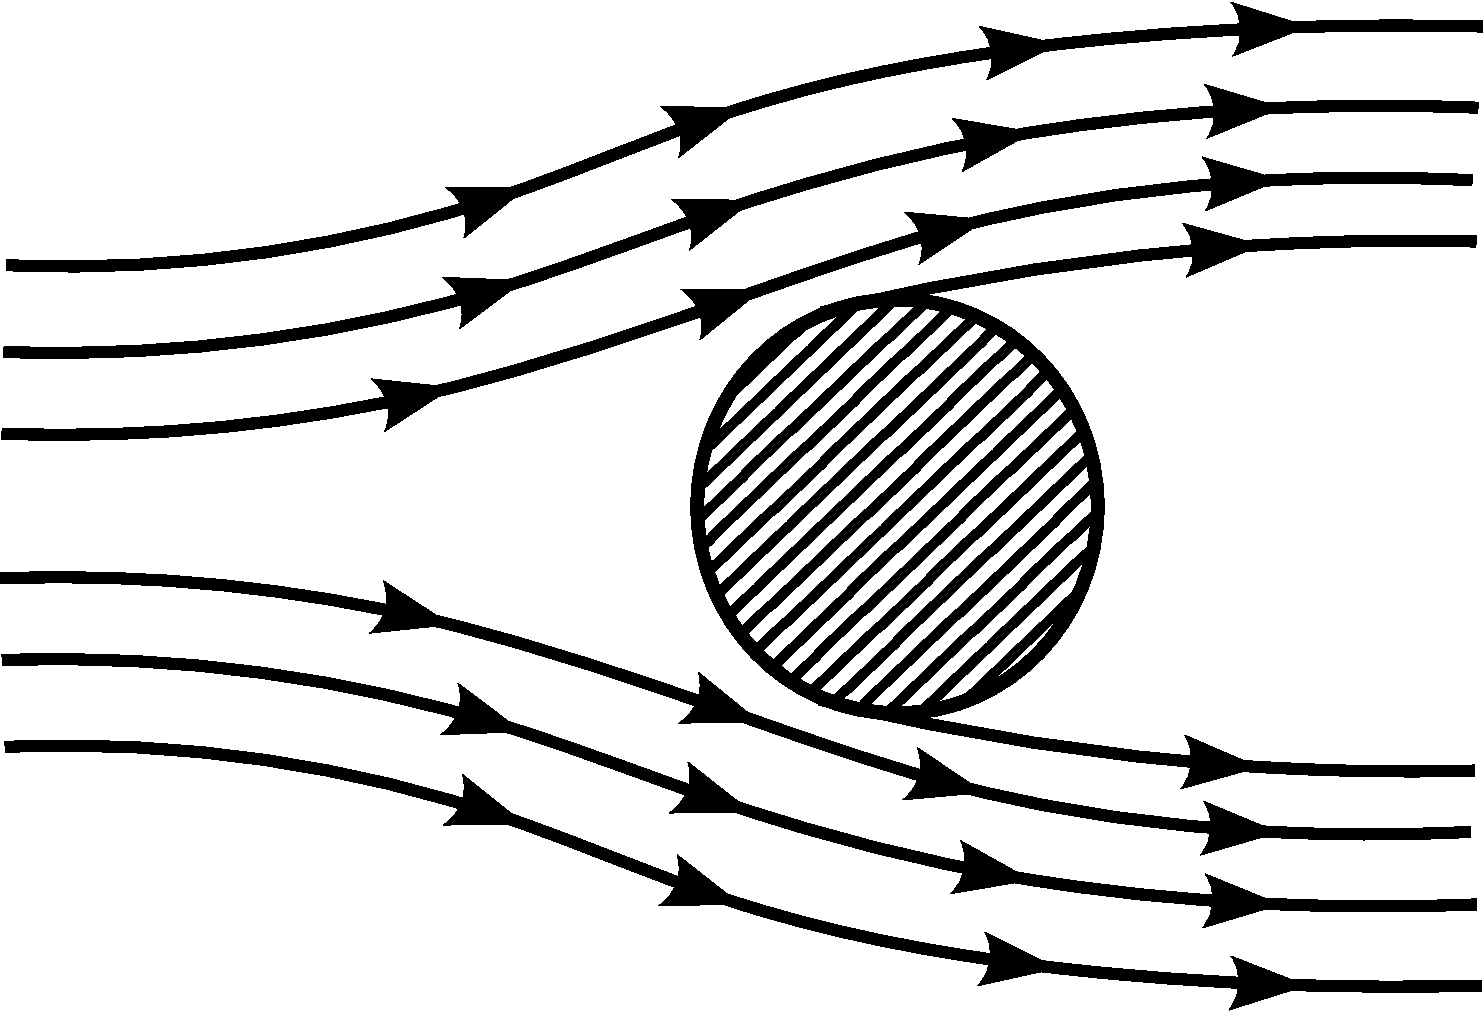
\includegraphics[width=6cm]{fig1}
  \caption{обтекание с поверхностью разрыва}
  \label{fig:f1}
\end{wrapfigure}

Аналогичным образом из закона сохранения циркуляции скорости можно было бы
сделать еще и следующий вывод. Предположим, что в некоторый момент времени
движение жидкости (во всем ее объеме) потенциально. Тогда циркуляция скорости по
любому замкнутому контуру в ней равна нулю \footnote{Для простоты мы считаем здесь,
что жидкость заполняет односвязную область пространства. Для могосвязной области
получился бы тот же самый конечный результат, но при рассуждениях надо было бы делать
специальные оговорки по поводу выбора контуров}. В силу теоремы Томсона можно было бы
заключить, что это будет иметь место и в течение всего дальнейшего времени, т.
е. мы получили бы результат, что если движение жидкости потенциально в некоторый
момент времени, то оно будет потенциальным и в дальнейшем (в частности, должно
было бы быть потенциальным всякое движение, при котором в начальный момент
времени жидкость вообще покоилась). Этому соответствует и тот факт, что
уравнение (\ref{eq:2.11}) удовлетворяется при $\rot\vv = 0$ тождественно.


В действительности, однако, все эти заключения имеют лишь весьма ограниченную
применимость. Дело в том, что приведенное выше доказательство сохранения
равенства $\rot\vv = 0$ вдоль линии тока, строго говоря, неприменимо для линии,
проходящей вдоль поверхности обтекаемого жидкостью твердого тела, уже просто
потому, что ввиду наличия стенки нельзя провести в жидкости замкнутый контур,
который охватывал бы собой такую линию тока. С этим обстоятельством связан тот
факт, что уравнения движения идеальной жидкости допускают решения, в которых на
поверхности обтекаемого жидкостью твердого тела происходит, как говорят, "отрыв
струй": линии тока, следовавшие вдоль поверхности, в некотором месте
"отрываются" от нее, уходя в глубь жидкости. В результате возникает картина
течения, характеризующаяся наличием отходящей от тела "поверхности
тангенциального разрыва", на которой скорость жидкости (будучи направлена в
каждой точке по касательной к поверхности) терпит разрыв непрерывности. Другими
словами, вдоль этой поверхности один слой жидкости как бы скользит по другому
(на Рис \ref{fig:f1} изображено обтекание с поверхностью разрыва, отделяющей движущуюся
жидкость от образующейся позади тела "застойной" области неподвижной жидкости).
С математической точки зрения скачок тангенциальной составляющей скорости
представляет собой, как известно, поверхностный ротор скорости.

При учете таких разрывных течений решение уравнений идеальной жидкости не
однозначно: наряду с непрерывным решением они допускают также и бесчисленное
множество решений с поверхностями тангенциальных разрывов, отходящими от любой
наперед заданной линии на поверхности обтекаемого тела. Подчеркнем, однако, что
все эти разрывные решения не имеют, физического смысла, так как тангенциальные
разрывы абсолютно неустойчивы, в результате чего движение жидкости становится в
действительности турбулентным (см.об этом в гл. III).

Реальная физическая задача об обтекании заданного тела, разумеется, однозначна.
Дело в том, что в действительности не существует строго идеальных жидкостей;
всякая реальная жидкость обладает какой-то, хотя бы и малой, вязкостью. Эта
вязкость может практически совсем не проявляться при движении жидкости почти во
всем пространстве, но сколь бы она ни была мала, она будет играть существенную
роль в тонком пристеночном слое жидкости. Именно свойства движения в этом (так
называемом пограничном) слое и определят в действительности выбор одного из
бесчисленного множества решений уравнений движения идеальной жидкости. При этом
оказывается, что в общем случае обтекания тел произвольной формы отбираются
именно решения с отрывом струй (что фактически приводит к возникновению
турбулентности).

Несмотря на все изложенное, изучение решений уравнений движения, соответствующих
непрерывному стационарному потенциальному обтеканию тел, имеет в некоторых
случаях смысл. Между тем как в общем случае обтекания тел произвольной формы
истинная картина течения практически ничего общего с картиной потенциального
обтекания не имеет, в случае тел, имеющих некоторую особую ("хорошо обтекаемую",
см. \S46). форму, движение жидкости может очень мало отличаться от
потенциального (точнее, оно будет не потенциальным лишь в тонком слое жидкости
вблизи поверхности тела и в сравнительно узкой области "следа" позади тела).

Другим важным случаем, когда осуществляется потенциальное обтекание, являются
малые колебания погруженного в жидкость тела. Легко показать, что если амплитуда
$a$ колебаний мала по сравнению с линейными размерами $l$ тела ($a\ll l$), то
движение жидкости вокруг тела будет всегда потенциальным. Для этого оценим
порядок величины различных членов в уравнении Эйлера
\[
   \pd{\vv}{t}+\vnv = - \nabla w
\]

Скорость у испытывает заметное изменение (порядка скорости $u$ колеблющегося
тела) на протяжении расстояний порядка размеров тела $l$. Поэтому производные от
$\vv$ по координатам — порядка величины $u/l$. Порядок же величины самой
скорости $\vv$ определяется (на не слишком болъших расстояниях от тела)
скоростью $u$. Таким образом, имеем $\vnv \sim u^2/l$. Производная же
$\partial{\vv}/\partial{t}$ — порядка величины $\omega u$, где $\omega$ -
частота колебаний. Поскольку ($\omega \sim u/a$, то имеем $\partial \vv/\partial
t \sim u^2/a$. Из $a \ll l$ следует теперь, что член $\vnv$ мал по сравнению с
$\partial \vv/\partial t$ и может быть опущен, так что уравнение движения
жидкости приобретает вид $\partial \vv/\partial t = - \nabla w$. Применив к
обеим сторонам этого уравнения операцию $\rot$, получаем:
\[
   \pdt \rot \vv = 0,
\]
откуда $\rot \vv = \const$. Но при колебательном движении среднее (по времени)
значение скорости равно нулю; поэтому из $\rot\vv = \const$ следует, $\rot\vv =
0$. Таким образом, движение жидкости, совершающей малые колебания, является (в
первом приближении) потенциальным.

Выясним теперь некоторые общие свойства потенциального движения жидкости. Прежде
всего напомним, что вывод закона сохранения циркуляции, а с ним и всех
дальнейших следствий, был основан на предположении об изэнтропичности течения.
Если же движение не изэнтропично, то этот закон не имеет места; поэтому, даже
если в некоторый момент времени движение является потенциальным, то в
дальнейшем, вообще говоря, завихренность все же появится. Таким образом,
фактически потенциальным может быть лишь изэнтропическое движение.

При потенциальном движении жидкости циркуляция скорости по любому замкнутому
контуру равна нулю:
\begin{equation}
   \label{eq:9.1}
   \oint \vv\;d\vect l = \int \rot \vv \; \df = 0
\end{equation}
Из этого обстоятельства следует, в частности, что при потенциальном течении не
могут существовать замкнутые линии тока \footnote{Этот результат, как и (\ref{eq:9.1}),
может не иметь места при движении жидкости в многосвязной области пространства.
При потенциальном течении в такой области циркуляция скорости может быть отличной
от нуля, если замкнутый контур, вдоль которого она берется, не может быть стянута
в точку так, чтобы нигде не пересечь границ области.}. Действительно, поскольку направление
линии тока совпадает в каждой точке с направлением скорости, циркуляция скорости
вдоль такой линии во всяком случае была бы отличной от нуля.

При вихревом же движении циркуляция скорости, вообще говоря, отлична от нуля. В
этом случае могут существовать замкнутые линии тока; надо, впрочем, подчеркнуть,
что наличие замкнутых линий тока отнюдь не является необходимым свойством
вихревого движения.

Как и всякое векторное поле с равным нулю ротором, скорость потенциально
движущейся жидкости может быть выражена в виде градиента от некоторого скаляра.
Этот скаляр называется \textit{потенциалом скорости}; мы будем обозначать его
посредством $\varphi$:
\begin{equation}
   \label{eq:9.2}
   \vv = \grad \varphi
\end{equation}
Написав уравнение Эйлера в виде (\ref{eq:2.10})
\[
   \pd{\vv}{t} + \frac{1}{2}\nabla v^2 - \vrv = - \nabla w
\]
и подставив в него $\vv = \nabla \varphi$, получаем:
\[
   \grad \left( \pd{\varphi}{t} + \frac{v^2}{2} + w \right) = 0,
\]
откуда находим следующее равенство:
\begin{equation}
   \label{eq:9.3}
   \pd{\varphi}{t} + \frac{v^2}{2} + w = f(t),
\end{equation}
где $f(t)$ - произвольная функция времени. Это равенство представляет собой
первый интеграл уравнений потенциального движения. Функция $f(t)$ в равенстве
(\ref{eq:9.3}) может быть без ограничения общности положена равной нулю за счет
неоднозначности в определении потенциала: поскольку скорость определяется
производными от $\varphi$ по координатам, можно прибавить к $\varphi$ любую
функцию времени.

При стационарном движении имеем (выбирая потенциал $\varphi$ не зависящим от
времени) $\partial\varphi/\partial t=0,\; f(t)=\const$, и (\ref{eq:9.3}) переходит в
уравнение Бернулли
\begin{equation}
   \label{eq:9.4}
   \frac{v^2}{2} + w = \const.
\end{equation}
Необходимо подчеркнуть здесь следующее существенное отличие между уравнениями
Бернулли в случае потенциального и непотенциального движений. В общем случае
произвольного движения const в правой части этого уравнения есть величина,
постоянная вдоль каждой данной линии тока, но, вообще говоря, различная для
разных линий тока. При потенциальном же движении const в уравнении Бернулли есть
величина, постоянная во всем объеме жидкости. Это обстоятельство в особенности
повышает роль уравнения Бернулли при исследовании потенциального движения.

 % Потенциальное движение
\section{Несжимаемая жидкость}
\label{sec:p10}

В очень многих случаях течения жидкостей (и газов) их плотность можно считать
неизменяющейся, т. е. постоянной вдоль всего объема жидкости в течение всего
времени движения. Другими словами, в этих случаях при движении не происходит
заметных сжатий или расширений жидкости. О таком движении говорят как о движении
\textit{несжимаемой жидкости}.

Общие уравнения гидродинамики сильно упрощаются при применении их к несжимаемой
жидкости. Правда, уравнение Эйлера не меняет своего вида, если положить в нем
$\rho = \const$, за исключением только того, что в уравнении (\ref{eq:2.4}) можно внести
$\rho$ под знак градиента:
\begin{equation}
   \label{eq:10.1}
   \pd{\vv}{t} + \vnv = - \nabla \frac{p}{\rho} + \vect g
\end{equation}
Зато уравнение непрерывности принимает при $\rho = \const$ простой вид
\begin{equation}
   \label{eq:10.2}
   \Div \vv = 0.
\end{equation}

Поскольку плотность не является теперь неизвестной функцией, как это имеет
место в общем случае, то в качестве основной системы уравнений гидродинамики
несжимаемой жидкости можно выбрать уравнения, содержащие только скорость.
Такими уравнениями являются уравнение непрерывности (\ref{eq:10.2}) и уравнение (\ref{eq:2.11}):
\begin{equation}
   \label{eq:10.3}
   \pdt \rot \vv = \rot \vrv.
\end{equation}

Уравнение Бернулли тоже может быть написано для несжимаемой жидкости в более
простом виде. Уравнение (\ref{eq:10.1}) отличается от общего уравнения Эйлера (\ref{eq:2.9}) тем,
что вместо $\nabla w$ в нем стоит $\nabla(p/\rho)$. Поэтому мы можем сразу
написать уравнение Бернулли, заменив просто в (\ref{eq:5.4}) тепловую функцию
отношением $p/\rho$:
\begin{equation}
   \label{eq:10.4}
   \frac{v^2}{2} + \frac{p}{\rho} + gz = \const.
\end{equation}
Для несжимаемой жидкости можно писать $p/\rho$ вместо $w$ также и в выражении
(\ref{eq:6.3}) для потока энергии, которое принимает тогда вид
\begin{equation}
   \label{eq:10.5}
   \rho \vv \left( \frac{p}{\rho} + \frac{v^2}{2} \right).
\end{equation}
Действительно, согласно известному термодинамическому соотношению имеем для
изменения внутренней энргии выражение $d\varepsilon = T\; ds - p\;dV$; при $s =
\const$ и $V=1/\rho = \const$ имеем $d\varepsilon=0$, т. е.
$\varepsilon=\const$. Поскольку же постоянные члены в энергии несущественны, то
можно опустить $\varepsilon$ и в $w=\varepsilon+p/\rho$.

В особенности упрощаются уравнения для потенциального течения несжимаемой
жидкости. Уравнение (\ref{eq:10.3}) удовлетворяется при $\rot \vv = 0$ тождественно.
Уравнение же (\ref{eq:10.2}) при подстановке $\vv = \grad \varphi$ превращается в
\begin{equation}
   \label{eq:10.6}
   \Delta \varphi = 0,
\end{equation}
т. е. в уравнение Лапласа для потенциала $\varphi$ \footnote{Потенциал скорости был
впервые введен \em{Эйлером}. Им же было получено для этой величины уравнение вида
\ref{eq:10.6}, получившее впоследствии название уравнения Лапласа.}. К этому уравнению должны
быть добавлены граничные условия на поверхностях соприкосновения жидкости с
твердыми телами: на неподвижных твердых поверхностях нормальная к поверхности
компонента $v_n$ скорости жидкости должна быть равна нулю, а в общем случае
движущихся твердых тел $v_n$ должна быть равна проекции скорости движения тела
на направление той же нормали (эта скорость является заданной функцией времени).
Скорость $v_n$ равна, с другой стороны, производной от потенциала $\varphi$ по
направлению нормали: $v_n = \pd{\varphi}{n}$. Таким образом, граничные условия
гласят в общем случае, что $\pd{\varphi}{n}$ является на границах заданной
функцией времени и координат.

При потенциальном движении скорость связана с давлением уравнением (\ref{eq:9.3}).
В случае несжимаемой жидкости в этом уравнении можно писать $p/\rho$ вместо $w$:
\begin{equation}
   \label{eq:10.7}
   \pd{\varphi}{t} + \frac{v^2}{2} + \frac{p}{\rho} = f(t).
\end{equation}

\begin{wrapfigure}{l}{6cm}
% "l" or "r" for the side on the page.
% And the width parameter for the width of the image space.
  \centering
  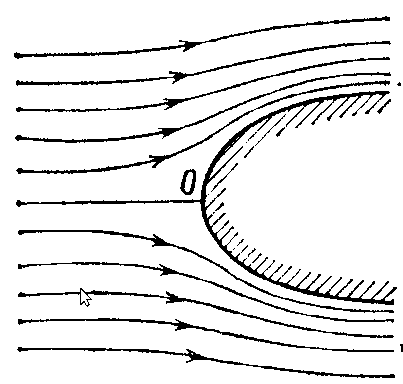
\includegraphics[width=6cm]{fig2}
  \caption{\label{fig:f2}}
\end{wrapfigure}

Отметим здесь следующее важное свойство потенциального движения несжимаемой
жидкости. Пусть через жидкость движется какое-нибудь твердое тело. Если
возникающее при этом течение жидкости является потенциальным, то это течение
зависит в каждый момент только от скорости движущегося тела в этот же момент
времени, но, например, не от его ускорения. Действительно, самое уравнение
(\ref{eq:10.6}) не содержит времени явно; время входит в решение лишь через граничные
условия, содержащие только скорость движущегося в жидкости тела.

Из уравнения Бернулли $v^2+p/\rho = \const$ видно, что при стационарном движении
несжимаемой жидкости (без поля тяжести) наибольшее значение давлений достигается
в точках, где скорость обращается в нуль. Такая точка обычно имеется на
поверхности обтекаемого жидкостью тела (точка $O$ на рис. 2) и называется
\textit{критической точкой}. Если $u$ - скорость натекающего на тело потока
жидкости (т. е. скорость жидкости на бесконечности), а $p_0$ - давление на
бесконечности, то давление в критической точке равно
\begin{equation}
   \label{eq:10.8}
   p_{max} = p_0 + \frac{\rho u^2}{2}.
\end{equation}

Если распределение скоростей в движущейся жидкости зависит только от двух
кородинат, скажем от $x$ и $y$, причем скорость параллельна везде плоскости
$xy$, то о таком течении говорят как о двухмерном или плоском. Для решения задач
о двухмерном течении несжимаемой жидкости иногда бывает удобным выражать
скорость через так называемую функцию тока. Из уравнения непрерывности
\[
   \Div \vv \equiv \pd{v_x}{x} + \pd{v_y}{y} = 0
\]
видно, что компоненты скорости могут быть написаны в виде производных
\begin{equation}
   \label{eq:10.9}
   v_x = \pd{\psi}{y},\; v_y = -\pd{\psi}{x}
\end{equation}
от некоторой функции $\psi(x,y)$, называемой \textit{функцией тока}. Уравнение
непрерывности при этом удовлетворяется автоматически. Уравнение же, которому
должна удовлетворять функция тока, получается подстановкой (\ref{eq:10.9}) в уравнение (\ref{eq:10.3})
\begin{equation}
   \label{eq:10.10}
   \pdt \nabla \psi -
   \pd{\psi}{x}\pd{\nabla\psi}{y}+
   \pd{\psi}{y}\pd{\nabla\psi}{x} = 0
\end{equation}

Зная функцию тока, можно непосредственно определить форму линий тока для
стационарного движения жидкости. Действительно, дифференциальное уравнение линий
тока (при двухмерном течении) есть
\[
   \frac{dx}{v_x} = \frac{dy}{v_y}
\]
или $v_y dx - v_x dy = 0$; оно выражает собой тот факт, что направление
касательной к линии тока в каждой точке совпадает с направлением скорости.
Подставляя сюда (\ref{eq:10.9}), получаем:
\[
   \pd{\psi}{x}dx + \pd{\psi}{y}dy = d\psi = 0,
\]
откуда $\psi = \const$. Таким образом, линии тока представляют собой семейство
кривых, получающихся приравниванием функции тока $\psi(x,y)$ произвольной
постоянной.

Если между двумя точками 1 и 2 в плоскости $x,y$ провести кривую, то поток
жидкости $Q$ через эту кривую определится разностью значений функции тока в этих
точках независимо от формы кривой. Действительно, если $v_n$ - проекция скорости
на нормаль к кривой в данной ее точке, то
\[
   Q = \rho \int_{1}^{2} v_n\;dl =
   \rho \int_{1}^{2} (-v_y\;dx + v_x\;dy) =
   \rho \int_{1}^{2} d\psi,
\]
или
\begin{equation}
   \label{eq:10.11}
   Q = \rho (\psi_2 - \psi_1).
\end{equation}
Мощные методы решения задач о плоском потенциальном обтекании несжимаемой
жидкостью различных профилей связаны с применением к ним теории функций
комплексного переменного\footnote{Подробное изложение этих методов и их многочисленных
применений может быть найдено во многих курсах и монографиях по гидродинамике с более
математическим уклоном. Здесь мы ограничимся лишь объяснением основной идеи метода}.
Основание для этих применений заключается в следующем.
Потенциал и функция тока связаны с компонентами скорости посредством
\footnote{Напомним, однако, что существование самой по себе функции тока связано
только с двумерностью течения, и отнюдь не требует его потенциальности.}
\[
   v_x=\pd{\varphi}{x}=\pd{\psi}{y},\; v_y = \pd{\varphi}{y}=-\pd{\psi}{x}.
\]
Но такие соотношения между производными функций $\varphi$ и $\psi$ с
математической точки зрения совпадают с известными условиями Коши-Римана,
выражающими собой тот факт, что комплексное выражение
\begin{equation}
   \label{eq:10.12}
   w = \varphi + i\psi
\end{equation}
является аналитической функцией комплексного аргумента $z=x+iy$. Это значит,
что функция $w(x)$ будет иметь в каждой точке определенную производную
\begin{equation}
   \label{eq:10.13}
   \D{w}{z} = \pd{\varphi}{x}+i \pd{\psi}{x} = v_x - iv_y.
\end{equation}

Функцию $w$ называют \textit{комплексным потенциалом}, а $\D{w}{z}$ -
комплексной скоростью. Модуль и аргумент последней определяют абсолютную
величину скорости $v$ и угол $\theta$ ее наклона к направлению оси $x$:
\begin{equation}
   \label{eq:10.14}
   \D{w}{z} = v e^{-i\theta}.
\end{equation}

На твердой поверхности обтекаемого контура скорость должна быть направлена по
касательной к нему. Другими словами, контур должен совпадать с одной из линий
тока, т. е. на нем должно быть $\psi = \const$; эту постоянную можно выбрать
равной нулю, и тогда задача об обтекании жидкостью заданного контура сводится к
определению аналитической функции $w(z)$, принимающей на этом контуре
вещественные значения. Более сложна постановка задачи в случаях, когда жидкость
имеет свободную поверхность (такой пример - см. задачу 9 к этому параграфу).

Интеграл от аналитической функции по какому-либо замкнутому контуру $C$ равен,
как известно, умноженной на $2\pi i$ сумме вычетов этой функции относительно ее
простых полюсов, расположенных внутри $C$; поэтому
\[
   \oint w'\;dz = 2\pi i \sum_{k} A_k,
\]
где $A_k$ - вычеты комплексной скорости. С другой стороны, имеем:
\begin{eqnarray}
   \oint w'\;dz =
   \oint (v_x - i v_y)(dx + i dy) = \\
   \oint (v_x dx + v_y dy) + i \oint (v_x dy - v_y dx).
\end{eqnarray}
Вещественная часть этого выражения есть не что иное, как циркуляция
$\bm\Gamma$ скорости по контуру $C$. Мнимая же часть (умноженная на $\rho$)
представляет собой поток жидкости через этот контур; при отсутствии внутри
контура источников жидкости этот поток равен нулю, и тогда имеем просто
\begin{equation}
   \label{eq:10.15}
   \bm\Gamma = 2\pi i \sum_{k} A_k
\end{equation}
(все вычеты $A_k$ при этом чисто мнимые).

Наконец, остановимся на условиях, при выполнении которых жидкость можно считать
несжимаемой. При адиабатическом изменении давления на $\Delta p$ плотность
жидкости изменится на
\[
   \Delta \rho = \ddp{\rho}{p}{s} \Delta p.
\]
Но согласно уравнению Бернулли колебания давления в стационарно движущейся
жидкости - порядка величины $\Delta p \sim \rho v^2$. Производная же
$\partial p/\partial \rho$ представляет собой (как мы увидим в \S64)
квадрат скорости звука $c$ в жидкости. Таким образом, находим оценку
\[
   \Delta \rho \sim \rho v^2/c^2.
\]
Жидкость можно считать несжимаемой, если $\Delta \rho / \rho \ll 1$. Мы видим,
что необходимым условием для этого является малость скорости ее движения по
сравнению со скоростью звука:
\begin{equation}
   \label{eq:10.16}
   v \ll c.
\end{equation}
Это условие достаточно, однако, только при стационарном движении. При
нестационарном движении необходимо выполнение еще одного условия. Пусть $\tau$ и
$l$ - величины порядка промежутков времени и расстояний, на которых скорость
жидкости испытывает заметное изменение. Сравнив члены $\partial \vv /\partial t$
и $\nabla p/\rho$ в уравнении Эйлера, получим, по порядку величины, $v/\tau \sim
\nabla p /l \rho$ или $\nabla p \sim l \rho v/\tau$, а соответствующее изменение
$\rho$ есть $\nabla \rho \sim l \rho v/ \tau c^2$. Сравнив теперь члены
$\partial \rho / \partial t$ и $\rho \Div \vv$ в уравнении непрерывности,
найдем, что производной $\partial \rho / \partial t$ можно пренебречь (т. е.
можно считать, что $\rho = \const$) в случае, если $\nabla \rho/\tau \ll \rho
v/l$ или
\begin{equation}
   \label{eq:10.17}
   \tau \gg \frac{l}{c}.
\end{equation}
Выполнение обоих условий (\ref{eq:10.16}) и (\ref{eq:10.17}) достаточно для того, чтобы можно было
считать жидкость несжимаемой. Условие (\ref{eq:10.17}) имеет наглядный смысл - оно
означает, что время $l/c$, в течение которого звуковой сигнал пройдет расстояние
$l$, мало по сравнению со временем $\tau$, в течение которого заметно изменяется
движение жидкости и, таким образом, дает возможность рассматривать процесс
распространения взаимодействий в жидкости как мгновенный.




\subsection*{Задачи}

\paragraph*{1}  Определить форму поверхности несжимаемой жидкости в поле
тяжести в цилиндрическом сосуде, вращаюш,емся вокруг своей оси с постоянной
угловой скоростью $\Omega$.

\texttt{Решение.} Ось $z$ выбираем по оси цилиндра. Тогда
$v_x=\Omega y, v_y=\Omega x, v_z = 0$. Уравнение непрерывности удовлетворяется
автоматически, а уравнение Эйлера (\ref{eq:10.1}) дает:
\[
   x\Omega^2 = \frac1{\rho}\pd{p}{x},\;
   y\Omega^2 = \frac1{\rho}\pd{p}{y},\;
   \frac1{\rho}\pd{p}{z} + g = 0.
\]Общий интеграл этих уравнений есть
\[
   \frac{p}{\rho} = \frac{1}{2}\Omega^2(x^2+y^2) - gz + \const.
\]
Ha свободной поверхности $p=\const$, так что эта поверхность является
параболоидом: $z = \left(\frac{\Omega^2}{2g}\right)(x^2)+y^2$
(начало координат - в низшей точке поверхности).

\paragraph*{2}  Шар (радиуса $R$) движется в несжимаемой идеальной жидкости
Определить потенциальное течение жидкости вокруг шара.

\texttt{Решение.} На бесконечности скорость жидкости должна обращаться в нуль.
Обращающимися на бесконечности в нуль решениями уравнения Лапласа $\nabla
\varphi = 0$ являются, как известно, $1/r$ и производные различных порядков от
$1/r$ по координатам (начало координат - в центре шара). Ввиду полной симметрии
шара в решение может войти лишь один постоянный вектор - скорость $\vect u$, а
ввиду линейности уравнения Лапласа и граничного условия к нему $\varphi$ должно
содержать и линейным образом. Единственным скаляром, который можно составить из
$\vect u$ н производных от $1/r$, является произведение $\vect u \nabla(1/r)$.
Соответственно этому ищем $\varphi$ в виде
\[
   \varphi = \vect A \nabla \frac1{r} = - \frac{\vect A \vect n}{r^2}
\]
($\vect n$ — единичный вектор в направлеини радиус-вектора). Постоянная
$\vect A$ определяется из условия равенства нормальных к поверхности шара
компонент скоростей $\vect v$ и $\vect u$ $(\mathbf{vn = un})$  при $r=R$.
Это условие дает $A=\vect u R^3/2$, так что
\[
   \varphi = - \frac{R^3}{2r^2}\vect{un},\;
   \vect v = \frac{R^3}{2r^3}\lbrack 3\vect{n(un)-u}\rbrack.
\]

Распределение давления определяется формулой (\ref{eq:10.7}):
\[
   p = p_0 - \frac{\rho v^2}{2} - \rho \pd{\varphi}{t}
\]
($p_0$ — давление на бесконечности). При вычислении производной
$\partial \varphi/\partial t$ надо иметь в виду, что начало координат
(выбранное нами в центре шара) смещается со временем со скоростью $u$. Поэтому
\[
   \pd{\varphi}{t} = \pd{\varphi}{\vect u}\dot{\vect u} - \vect u \nabla \varphi.
\]
Распределение давления иа поверхности шара даетси формулой
\[
   p = p_0 + \frac{\rho u^2}{8}(9\cos^2\theta - 5) + \frac{\rho}{2}R\vect n \D{\vect u}{t}
\]
($\theta$ - угол между $\vect n$ и $\vect u$).

\paragraph*{3}
То же для бесконечного цилиндра, движущегоси перпендикулярно к своей оси
\footnote{Решение более общих задач о потенциальном обтекании эллипсоида и цилиндра
эллиптического сечения см. в книгах:

\em{Кочин Н.Е., Кибель И.А., Розе Н.В.}, Теоретическая гидромеханика. - Физматгиз, 1963,
ч. 1, гл. VII; \em{Лэмб Г.} Гидродинамика. - М.: Гостехиздат, 1947, \S\S103-116
(\em{Lamb H.} Hydrodynamics. - Cambridge, 1932)}.

\texttt{Решение.} Течение не зависит от координаты вдоль оси цилиядра, так что
приходится решать двухмерное уравнение Лапласа. Обращающимися в нуль на
бесконечности решениями являются производные от $\ln r$ по координатам,
начиная от первого порядка и выше ($\vect r$ — перпендикулярный к оси цилиндра
радиус-вектор). Ищем решение в виде
\[
   \varphi = \vect A \nabla \ln r = \frac{\vect{An}}{r}
\]
и с помощью граничных условий получаем $\vect A = -R^2 \vect u$, так что
\[
   \varphi = - \frac{R^2}{r}\vect{un},\;
   v = \frac{R^2}{r^2}\lbrack 2 \vect{n(un)-u} \rbrack.
\]
Давление на поверхности цилиндра дается формулой
\[
   p = p_0 + \frac{\rho u^2}{2}(4\cos^2\theta - 3) + pR\vect n\D{\vect u}{t}
\]

\paragraph*{4}

Определить потенциальное движение идеальной несжимаемой жидкости в
эллипсоидальном сосуде, вращающемся вокруг одной из своих главных осей с угловой
скоростью $\Omega$; определить полный момент импульса жидкости в сосуде.

\texttt{Решение.} Выбираем декартовы координаты $x,y,z$ вдоль осей эллипсоида в
данный момент времени; ось вращения совпадает с осью $z$. Скорость Стенки сосуда
есть $\vect u = \lbrack \Omega \vect r \rbrack$, так что граничное условие
$v_n=\partial\varphi/\partial n=u_n$ есть
\[
   \pd{\varphi}{n} = \Omega(xn_y-yn_x),
\]
или, используя уравнение эллипсоида $x^2/a^2+y^2/b^2+z^2/c^2=1$:
\[
   \frac{x}{a^2}\pd{\varphi}{x} +
   \frac{y}{b^2}\pd{\varphi}{y} +
   \frac{z}{c^2}\pd{\varphi}{z} =
   xy\Omega\left(\frac1{b^2}+\frac1{a^2}\right)
\]
Решение уравнение Лапласа, удовлетворяющее этому условию, есть
\begin{equation}
   \label{eq:10_tasks_1}
   \varphi = \Omega \frac{a^2-b^2}{a^2+b^2}xy.
\end{equation}
Момент импульса жидкости в сосуде
\[
   M = \rho \int (xv_y-yv_x)dV.
\]
Интегрируя по объему эллипсоида, получаем
\[
   M = \frac{\Omega \rho V}{5}\frac{(a^2-b^2)^2}{a^2+b^2}.
\]

Формула (\ref{eq:10_tasks_1}) определяет абсолютное движение жидкости, отнесенное к мгновенному
положению осей $x,y,z$, связанных с вращающимся сосудом. Движение же
относительно сосуда (т, е, относительно вращающейся системы координат $x,y,z$),
получится вычитанием скорости $\lbrack \vect{\Omega r} \rbrack$ из абсолютной
скорости жидкости; обозначив относительную скорость жидкости $v'$, имеем
\[
   v'_x = \pd{\varphi}{x}+\Omega y = \frac{2\Omega a^2}{a^2+b^2}y,
   v'_y = - \frac{2\Omega b^2}{a^2+b^2}x,
   v'_z = 0.
\]
Траектории относительного движения получаются путем интегрирования уравнений
$\dot x = v'_x, \; \dot y = v'_y$ и представляют эллипсы
$x^2/a^2+y^2/b^2 = \const$, подобные граничному эллипсу.

\paragraph*{5}
Определить течение жидкости вблизи критической точки на обтекаемом теле (рис. 2).

\texttt{Решение.} Малый участок поверхности тела вблизи критической точки можно
рассматривать как плоский. Выбираем его в качестве плоскости $xy$. Разлагая
$\varphi$ при малых $x,y,z$ в ряд, имеем с точностью до членов второго порядка;
\[
   \varphi = ax + by + cz + Ax^2 + By^2 + Dxy + Eyz + Fxz
\]
(постоянный член в $\varphi$ несуществен). Постоянные коэффициенты определяем
так, чтобы $\varphi$ удовлетворяло уравнению $\nabla \varphi = 0$ и граничным
условиям $v_z = \partial \varphi/\partial z$ при $z = 0$ и всех $x,y$ и
$\partial \varphi/\partial x = \partial \varphi/\partial y = 0$ при
$x=y=z=0$ (в критической точке).  Это дает
\[
   a=b=c=0;\; C=-A-B, E=F=0.
\]

\begin{wrapfigure}{l}{6cm}
  \centering
  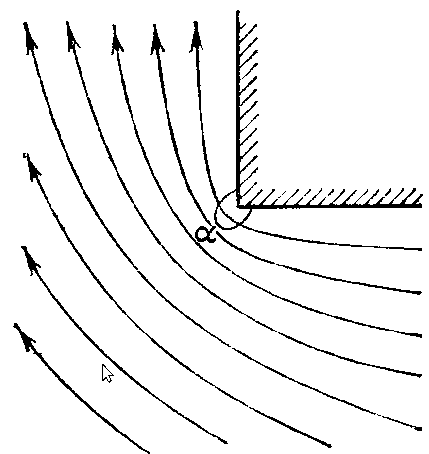
\includegraphics[width=6cm]{fig3}
  \caption{\label{fig:f3}}
\end{wrapfigure}

Член $Dxy$ может быть всегда исключен соответствующим поворотом осей $x$ и $y$.
В результате получаем:
\begin{equation}
   \label{eq:10t2}
   \varphi = Ax^2+By^2-(A+B)z^2.
\end{equation}
Если течение обладает аксиальной симметрией вокруг оси $z$ (симметричное
 обтекание тела вращения), то должно быть $A = B$, так что
\begin{equation}
   \label{eq:10t3}
   \varphi = A(x^2 + y^2 -2z^2).
\end{equation}
Компоненты скорости равны
\[
   v_x = 2Ax,
   v_y = 2Ay,
   v_z = -4Az,
\]
Линии тока определяются уравнениями (\ref{eq:5.2}), откуда $x^2z=c_1,\;y^2z=c_2$, т.е.
линии тока являются кубическими гиперболами.

Если течение является однородным вдоль оси $y$ (например, при обтекании в
направлении оси $z$ цилиндра с осью вдоль оси $y$), то в (\ref{eq:10t2}) должно быть $B=0$,
так что
\[
   \varphi = A(x^2 - z^2).
\]
Линиями тока являются гиперболы $xz = \const$.

\paragraph*{6}
Определить движение жидкости при потенциальном обтекании угла, образованного
двумя пересекающимися плоскостями  (вблизи вершины угла).

\texttt{Решение.} Выбираем полярные координаты $r,\theta$ в плоскости
поперечного сечеиия, перпендикулярной к линии пересечения плоскостей, с началом
в вершине угла. Угол $\theta$ отсчитывается от одной из прямых, образующих
сечение угла. Пусть $\alpha$ есть величина обтекаемого угла; при $\alpha<\pi$
течение происходит внутри угла, при $\alpha>\pi$ - вне его. Граничное условие
исчезновения нормальной составляющей скорости гласит $d\varphi/d\theta = 0$ при
$\theta = 0$ и $\alpha$. Удовлетворяющее этому условию решение уравнения Лапласа
пишем в виде \footnote{Выбираем решение с наиболее низкой (малые $r$!) положительной степенью $r$.}
\[
   \varphi = Ar^n\cos n\theta,\; n = \pi/\alpha,
\]
так что
\[
   v_r = nAr^{n-1}\cos n\theta,\; v_{\theta}=-nA^{n-1}\sin n\theta.
\]
При $n<1$ (обтекание выпуклого угла; рис. 3) $v$ обращается в начале координат
в бесконечность как $r^{-(1-n)}$. При $n>1$ (течение внутри вогнутого
угла - рис, 4) $v$; обращается при $r=0$ в нуль.

\begin{wrapfigure}{r}{6cm}
  \centering
  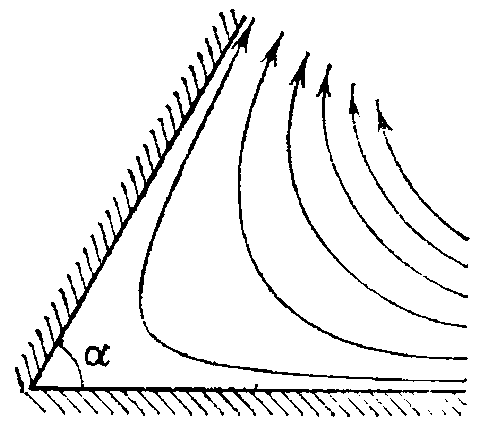
\includegraphics[width=6cm]{fig4}
  \caption{\label{fig:f4}}
\end{wrapfigure}

Функция тока, определяющая форму линий тока, есть
\[
   \psi = Ar^n \sin n\theta.
\]
Полученные для $\varphi$ п $\psi$ выражения являются вещественной и мнимой
частями комплексного по-тенииала $w = Az^n$ \footnote{Задачи 5 и 6, если рассматривать
граничные плоскости в них как бесконечные, вырождены в том смысле, что значения постоянных
коэффициентов $A,B$ в нх решениях остаются неопределенными. В реальных случаях обтекания
конечных тел эти значения определяются условиями задачи в целом.}.

\paragraph*{7}
Из несжимаемой жидкости, заполняющей все пространство, внезапно удаляется
сферический объем радиуса $a$. Определить время, в течение которого
образоваишаяся полость заполнится жидкостью  (\textit{Besant}, 1859;
\textit{Rayleigh}, 1917).

\texttt{Решение.} Движение жидкости после образования полости будет
центрально-симметрическим со скоростями, иаправлеииыми  в каждой точке по
 радиусу к центру.  Для радиальной скорости
\[
   v_r \equiv v<0
\]
имеем уравнение Эйлера (в сферических координатах)
\begin{equation}
   \label{eq:10t4}
   \pd{v}{t} + v \pd{v}{r} = - \frac1{\rho} \pd{p}{r}.
\end{equation}
Уравнение непрерывности дает:
\begin{equation}
   \label{eq:10t5}
   r^2v = F(t),
\end{equation}
где  $F(t)$ - произвольная функция времени; это равенство выражает собой тот
факт, что в силу несжимаемости жидкости объем, протекающий через сферу любого
радиуса, не зависит от последнего.

Подставляя $v$; из (\ref{eq:10t4}) в (\ref{eq:10t5}), имеем:
\[
   \frac{F'(t)}{r^2} + v \pd{v}{r} = - \frac1{\rho} \pd{p}{r},
\]
Интегрируя это уравнение по $r$ в пределах от $\infty$ до радиуса
\[
   R = R(t) \leq a
\]
заполняющейся полости, получим:
\begin{equation}
   \label{eq:10t6}
   - \frac{F'(t)}{R(t)} + \frac{V^2}{2} = \frac{p_0}{\rho},
\end{equation}
где $V = dR(t)/dt$ - скорость изменения радиуса полости, а $p_0$ - давление на
бесконечности; скорость жидкости на бесконечности, а также давление на
поверхности полости равны нулю. Написав соотношение (\ref{eq:10t5}) для точек на поверхности
полости, находим:
\[
   F(t) = R^2(t)V(t).
\]
и, подставив это выражение для $F(t)$ в (\ref{eq:10t6}), получим следующее уравнение
\begin{equation}
   \label{eq:10t7}
   - \frac{2V^2}{2} - \frac{1}{2} R \D{V^2}{R} = \frac{p_0}{\rho}.
\end{equation}
в этом уравнении переменные разделяются и, интегрируя его при начальном условии
$V=0$ при $R=a$ (в начальный момент жидкость покоилась), найдем:
\[
   V = \D{R}{t} = - \sqrt{\frac{2p_0}{3\rho}\left(\frac{a^3}{R^3}-1\right)}.
\]
Отсюда имеем для искомого полного времени заполнения полости:
\[
   \tau = \sqrt{\frac{3\rho}{2p_0}}\int_0^a{\frac{dR}{\sqrt{(a/R)^3}-1}}.
\]
Этот интеграл приводится к виду $B$-интеграла Эйлера, и вычисление дает
окончательно:
\[
   \tau = \sqrt{\frac{3a^2 \rho \pi}{2p_0}} \frac{\Gamma(5/6)}{\Gamma(1/3)} =
   0,915a \sqrt{\frac{\rho}{p_0}}.
\]

\paragraph*{8}
Погруженная в несжимаемую жидкость сфера расширяется по заданному закону
$R=R(t)$. Определить давление жидкости на поверхности сферы.

\texttt{Решение.} Обозначим искомое давление посредством $P(t)$. Вычисления в
точности аналогичны произведенным в предыдущей задаче с той лишь разницей, что
при $r=R$ давление равно не нулю, а $P(t)$. В результате получим вместо
(3) уравнение
\[
   - \frac{F'(t)}{R(t)} + \frac{V^2}{2} = \frac{p_0}{\rho} - \frac{P(t)}{\rho}
\]
и соответственно вместо (4) уравнение
\[
   \frac{p_0 - P(t)}{\rho} = - \frac{3V^2}{2} - RV \D{V}{R}.
\]
Имея в виду, что $V=dR/dt$, можно привести выражение для $P(t)$ к виду
\[
   P(t) = p_0 + \frac{\rho}{2}\left\lbrack \frac{d^2(R^2)}{dt^2} +
   \left( \D{R}{t} \right)^2 \right\rbrack.
\]

\paragraph*{9}
Определить  форму  струн,  вытекающей   из   бесконечно  длинной   щели
прорезанной в плоской стенке.
\texttt{Решение.} Пусть в плоскости $x,y$ стенка совпадает с осью $x$,
отверстие есть отрезок $-a/2 \leq x \leq a/2$ этой оси, а жидкость занимает
полуплоскость $y>0$. Вдали от стенки (при $y \to \infty$) скорость жидкости
равна нулю, а давление пусть будет $p_0$.

\begin{figure}[hb]
  \centering
  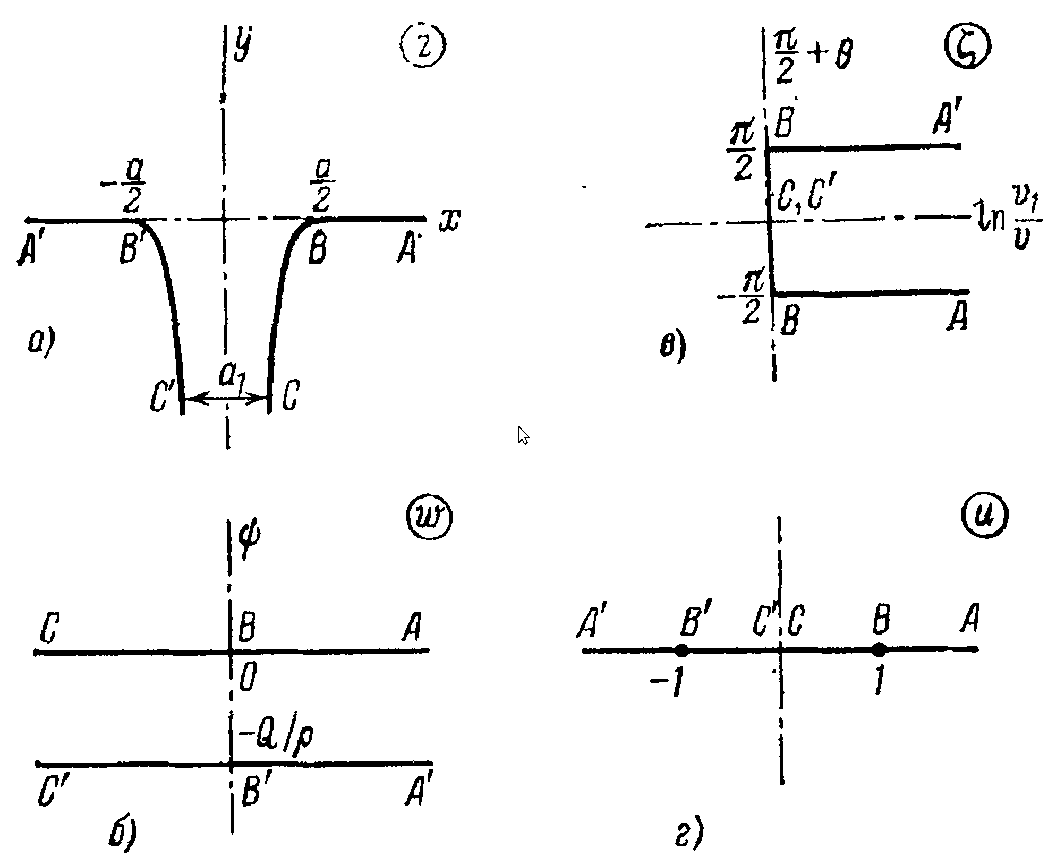
\includegraphics[width=9cm]{fig5}
  \caption{\label{fig:f5}}
\end{figure}

На свободной поверхности струя ($BC$ и $B'C'$ на рис. 5,а) давление $p=0$, а
скорость согласно уравнению Бернулли имеет постоянную величину $v_1 =
\sqrt{2p_0/\rho}$. Линии стенки, продолжающиеся в свободную границу струи,
представляют собой линии тока. Пусть на лниии $ABC$ $\psi = 0$; тогда на линии
$A'B'C'$ $\psi = -Q/\rho$. Где $Q = \rho a_1 v_1$ - расход жидкости в струе
($a_1$, $v_1$ - ширина струн и скорость жидкости в ней на бесконечности).
Потенциал $\varphi$ меняется как на линии $ABC$, так и на линии $A'B'C'$ от
$-\infty$ до $+\infty$; пусть в точках $B$ и $B' \varphi = 0$, Тогда в плоскости
комплексного переменного $w$ области течения будет соответствовать бесконечная
полоса ширины $Q/\rho$ (обозначения точек на рис, 5,б - г соответствуют
обозначениям на рис, 5,а в плоскости $x,y$). Введем новую комплексную переменную
- логарифм комплексной скорости:
\begin{equation}
   \label{eq:10t9.1}
   \zeta = - \ln \left\lbrack \frac1{v_1 e^{i\pi/2}} \D{w}{z} \right\rbrack =
   \ln \frac{v_1}{v} + i \left( \frac{\pi}{2} + \theta \right)
\end{equation}
($v_1 e^{i\pi/2}$ - комплексная скорость на бесконечности струи). На $A'B'$
имеем $\theta = 0$; на $AB \theta = - \pi$ на $BC$ и $B'C'$ $v=v_1$, причем на
бесконечности струн $\theta = - \pi/2$. Поэтому в плоскости переменного $\zeta$
области течения соответствует полуполоса ширины $\pi$, расположенная в правой
полуплоскости (рис, 5, в). Если мы теперь найдем конформное преобразование,
переводящее полосу плоскости $w$ в полуполосу плоскости $\zeta$ (с указанным на
рис. 5 соответствием точек), то тем самым мы определим $w$ как функцию от
$dw/dz$; функция $w$ может быть найдена затем одной квадратурой.

Для того чтобы найти искомое преобразование, введем еще одну вспомогательную
комплексную переменную $u$, такую, чтобы в плоскости $u$ области течения
соответствовала верхняя полуплоскость, причем точкам $B$ и $B'$ соответствуют
точки $u=\pm 1$, точкам $C,C'\; u = 0$, а бесконечно удаленным точкам $A$ и $A'$
$u = \pm \infty$ (рис, 5,г). Зависимость $w$ от этой вспомогательной переменной
определяется конформным преобразованием, переводящим верхнюю полуплоскость $u$ в
полосу плоскости $w$. При условленном соответствии точек это есть
\begin{equation}
   \label{eq:10t9.2}
   w = - \frac{Q}{\rho\pi}\ln u
\end{equation}
Чтобы найти зависимость $\zeta$ от $u$, надо найти конформное отображение
полуполосы плоскости $\zeta$, в верхнюю полуплоскость $u$. Рассматривая эту
полуполосу как треугольник, одна из вершин которого удалена в бесконечность,
можно найти искомое отображение с помощью известной формулы Шварца-Кристоффеля;
ответ гласит
\begin{equation}
   \label{eq:10t9.3}
   \zeta = - i \arcsin u.
\end{equation}
Формулы (\ref{eq:10t9.2}), (\ref{eq:10t9.3}) решают задачу, определяя в параметрическом виде зависимость
$dw/dz$ от $w$.

Определим форму струи. На $BC$ имеем
$w = \varphi,\; \zeta = i \left( \frac{\pi}{2}+\theta \right) $, а $u$
меняется между 0 и 1. Из (\ref{eq:10t9.2}) и (\ref{eq:10t9.3}) получим:
\begin{equation}
   \label{eq:10t9.4}
   \varphi = - \frac{Q}{\rho \pi}\ln (-\cos \theta),
\end{equation}
а из (1) $d\varphi/dz = v_1 e^{-i\theta}$, или
\[
   dz \equiv dx + i\; dy = \frac1{v_1} e^{i\theta}d\varphi =
   \frac{a_1}{\pi} e^{i\theta} \tan \theta\; d\theta,
\]
откуда интегрированием (с условиями $y=0, x=a/2$ при $\theta = - \pi$) найдем
в параметрическом виде форму струи, В частности, для сжатия струи получается
$a_1/a = \pi/(2+\pi) = 0,61$.


 % Несжимаемая жидкость
\section{Сила сопротивления при потенциальном обтекании}
\label{sec:p11}

Рассмотрим задачу о потенциальном обтекании несжимаемой идеальной жидкостью
какого-либо твердого тела. Такая задача, конечно, полностью эквивалентна задаче
об определении течения жидкости при движении через нее того же тела. Для
получения второго случая из первого достаточно перейти к системе координат, в
которой жидкость на бесконечности покоится. Мы будем говорить ниже именно о
движении твердого тела через жидкость.

Определим характер распределения скоростей в жидкости на больших расстояниях от
движущегося тела. Потенциальное движение несжимаемой жидкости определяется
уравнением Лапласа $\nabla \varphi = 0$. Мы должны рассмотреть такие решения
этого уравнения, которые обращаются на бесконечности в нуль, поскольку жидкость
на бесконечности неподвижна. Выберем начало координат где-нибудь внутри
движущегося тела (эта система координат движется вместе с телом; мы, однако,
рассматриваем распределение скоростей в жидкости в некоторый заданный момент
времени). Как известно, уравнение Лапласа имеет решением $1/r$, где $r$ -
расстояние от начала координат. Решением являются также градиент $\nabla(1/r)$ и
следующие производные от $1/r$ по координатам. Все эти решения (и их линейные
комбинации) обращаются на бесконечности в нуль. Поэтому общий вид искомого
решения уравнения Лапласа на больших расстояниях от тела есть
\[
   \varphi = - \frac{a}{r} + \vect A \nabla \frac1{r} + \dots ,
\]
где $a$, $\vect A$ не зависят от координат; опущенные члены содержат
производные высших порядков от $1/r$. Легко видеть, что постоянная $a$ должна
быть равной нулю. Действительно, потенциал $\varphi = -a/r$ дает скорость
\[
   \vect v = - \nabla \frac{a}{r} = \frac{a \vect r}{r^3}.
\]
Вычислим соответствующий поток жидкости через какую-нибудь замкнутую
поверхность, скажем, сферу с радиусом $R$. На этой поверхности скорость
постоянна и равна $a/R^2$; поэтому полный поток жидкости через нее равен
$\rho(a/R^2)4\pi R^2 = 4\pi \rho a$. Между тем, поток несжимаемой жидкости
через всякую замкнутую поверхность должен, очевидно, обращаться в нуль. Поэтому
заключаем, что должно быть $a = 0$.

Таким образом, $\varphi$ содержит члены, начиная с членов порядка $1/r^2$.
Поскольку мы ищем скорость на больших расстояниях, то члены более высоких
порядков можно опустить, и мы получаем:
\begin{equation}
   \label{eq:11.1}
   \varphi = \vect A \nabla \frac1{r} = - \frac{\vect{An}}{r^2},
\end{equation}
а для скорости $\vect v = \grad \varphi$
\begin{equation}
   \label{eq:11.2}
   \vect v = (\vect A \nabla) \nabla \frac1{r} = \frac{3\vect{(An)n - A})}{r^3}
\end{equation}
($\vect n$ — единичный вектор в направлении $\vect r$). Мы видим, что на больших
расстояниях скорость падает, как $1/r^3$. Вектор $\vect A$ зависит от конкретной
формы и скорости движения тела и может быть определен только путем полного
решения уравнения $\nabla \varphi = 0$ на всех расстояниях, с учетом
соответствующих граничных условий на поверхности движущегося тела.

Входящий в (\ref{eq:11.2}) вектор $\vect A$ связан определенным образом с полным
импульсом и с полной энергией жидкости, обтекающей движущееся в ней тело. Полная
кинетическая энергия жидкости (внутренняя энергия несжимаемой жидкости
постоянна) есть
\[
   E = \frac{\rho}{2}\int v^2\; dV,
\]
где интегрирование производится по всему пространству вне тела. Выделим из
пространства часть $V$, ограниченную сферой большого радиуса $R$, с центром в
начале координат и будем интегрировать сначала только по объему $V$, имея в виду
стремить затем $R$ к бесконечности. Имеем тождественно
\[
   \int v^2\; dV = \int u^2\; dV + \int \vect{(v+u)(v-u)\;dV},
\]
где $\vect u$ - скорость тела. Поскольку $u$ есть не зависящая от координат
величина, то первый интеграл равен просто $u^2(V-V_0)$, где $V_0$ - объем тела.
Во втором же интеграле пишем сумму $\vect{v+u}$ в виде
$\nabla(\varphi+\vect{ur})$ и, воспользовавшись также тем, что $\Div \vv =0$ в
силу уравнения непрерывности, а $\Div \vect u \equiv 0$, имеем:
\[
   \int v^2\; dV = u^2(V-V_0) + \int \Div \lbrace \vect{(\varphi + ur)(v-u)} \rbrace dV.
\]
Второй интеграл преобразуем в интеграл по поверхности $S$ сферы и поверхности $S_0$
тела:
\[
   \int v^2\; dV = u^2(V-V_0) + \oint_{S+S_0} \vect{(\varphi+ur)(v-u)}\;\df .
\]
На поверхности тела нормальные компоненты $\vv$ и $\vect u$ равны друг другу в
силу граничных условий; поскольку вектор $\df$ направлен как раз по нормали к
поверхности, то ясно, что интеграл по $S_0$ тождественно обращается в нуль. На
удаленной же поверхности $S$ подставляем для $\varphi$ и $\vv$ выражения
(\ref{eq:11.1} - \ref{eq:11.2}) и опускаем члены, обращающиеся в нуль при переходе к пределу по $R \to
\infty$. Написав элемент поверхности сферы $S$ в виде $\df = \vect n R^2\; do$,
где $do$ — элемент телесного угла, получим:
\[
   \int v^2\; dV = u^2 \left( \frac{4\pi}{3}R^3 - V_0 \right) +
   \int \lbrace 3 \vect{(An)(un) - (un)^2}R^3 \rbrace\; do .
\]
Наконец, произведя интегрирование
\footnote{
Интегрирование по $do$ эквивалентно усреднению подинтегрального выражения по всем
направлениям вектора $\vect n$ и умножению затем на $4\pi$. Для усреднения выражений
типа $(\vect{An})(\vect{Bn}) \equiv A_i n_i B_k n_k$ ($\vect{A,B}$ - постоянные векторы),
пишем
\[
\overline{\vect{(An)(Bn)}} = A_i B_k \overline{n_i n_k} =
\frac1{3} \delta_{ik} A_i B_k = \frac1{3}\vect{AB}.
\]
}
и умножив на $\rho/2$, получаем окончательно
следующее выражение для полной энергии жидкости:
\begin{equation}
   \label{eq:11.3}
   E = \frac{\rho}{2}(4\pi \vect{Au} - V_0 u^2) .
\end{equation}

Как уже указывалось, точное вычисление вектора $\vect A$ требует полного решения
уравнения $\nabla \varphi = 0$ с учетом конкретных граничных условий на
поверхности тела. (Эбщий характер зависимости $\vect A$ от скорости $\vect u$
тела можно, однако, установить уже непосредственно из факта линейности уравнения
для $\varphi$ и линейности (как по $\varphi$, так и по $\vect u$) граничных
условий к этому уравнению. Из этой линейности следует, что $\vect A$ должно быть
линейной же функцией от компонент вектора $u$. Определяемая же формулой (\ref{eq:11.3})
энергия $E$ является, следовательно, квадратичной функцией компонент вектора
$\vect u$ и потому может быть представлена в виде
\begin{equation}
   \label{eq:11.4}
       E = \frac{m_{ik}u_i u_k}{2},
\end{equation}


где $m_{ik}$ - некоторый постоянный симметрический тензор, компоненты которого
могут быть вычислены с помощью компонент вектора $\vect A$; его называют
тензором \textit{присоединенных масс}.

Зная энергию $E$, можно получить выражение для полного импульса $\vect P$
жидкости. Для этого замечаем, что бесконечно малые изменения $E$ и $\vect P$
связаны друг с другом соотношением $dE = \vect u\; d\vect P$
\footnote{
Действительно, пусть тело ускоряется под влиянием какой-либо внешней силы $F$.
В результате импульс жидкости будет возрастать; пусть $d\vect{P}$ есть его приращение
в течение времени $dt$. Это приращение связано с силой посредством $d\vect{P} = \vect{F}dt$,
в умноженное на скорость $\vect u$ дает $\vect u d \vect P$, т.е. работу силы $\vect F$ на
пути $\vect u dt$, которая в свою очередь должна быть равна увеличению энергии $dE$ жидкости.

Следует заметить, что вычисление импульса непосредственно как интеграла $\int \rho \vect v dV$
по всему объему жидкости было бы невозможным. Дело в том, что этот интеграл (со скоростью $\vect v$, распределенной по (\ref{eq:11.2})) расходится в том смысле, что результат интегрирования, хотя и конечен, но зависит от способа взятия интеграла: производя
интегрирование по большой области, размеры которой устремляют затем к бесконечности, мы
получили бы значение, зависящее от формы области (сфера, цилиндр и т.п.). Используемый же
нами способ вычисления импульса, исходя из соотношения $u \vect P = dE$, приводит ко
воплне определенному конечному значению (даваемому формулой (\ref{eq:11.6}),
заведомо удовлетворящему физическому условию о связи изменения импульса с действующим на тело
силами.
}; отсюда следует,
что если $E$ выражено в виде (\ref{eq:11.4}), то компоненты $\vect P$ должны иметь вид
\begin{equation}
   \label{eq:11.5}
       P_i = m_{ik} u_k .
\end{equation}
Наконец, сравнение формул (\ref{eq:11.3} - \ref{eq:11.5}) показывает, что $\vect P$ выражается
через $\vect A$ следующим образом:
\begin{equation}
   \label{eq:11.6}
   \vect P = 4\pi \rho \vect A - \rho V_0 \vect u.
\end{equation}
Следует обратить внимание на то, что полный импульс жидкости оказывается вполне
определенной конечной величиной.

Передаваемый в единицу времени от тела к жидкости импульс есть $d\vect P/dt$.
Взятый с обратным знаком, он определяет, очевидно, реакцию $\vect F$ жидкости,
т. е. действующую на тело силу:
\begin{equation}
   \label{eq:11.7}
       \vect F = - \D{\vect P}{t}.
\end{equation}
Параллельная скорости тела составляющая $\vect F$ называется \textit{силой
сопротивления}, а перпендикулярная составляющая - \textit{подъемной силой}.

Если бы было возможно потенциальное обтекание равномерно движущегося в идеальной
жидкости тела, то было бы $\vect P = \const$ (так как $\vect u = \const$) и
$\vect F = 0$. Другими словами, отсутствовала бы как сила сопротивления, так и
подъемная сила, т. е. действующие на поверхность тела со стороны жидкости силы
давления взаимно компенсируются (так называемый парадокс Даламбера).
Происхождение этого "парадокса" в особенности очевидно для силы сопротивления.
Действительно, наличие этой силы при равномерном движении тела означало бы, что
для поддержания движения какой-либо внешний источник должен непрерывно
производить работу, которая либо диссипи-руется в жидкости, либо преобразуется в
ее кинетическую энергию, приводя к постоянно уходящему на бесконечность потоку
энергии в движущейся жидкости. Но никакой диссипации энергии в идеальной
жидкости, по определению, нет, а скорость приводимой телом в движение жидкости
настолько быстро убывает с увеличением расстояния от тела, что никакого потока
энергии на бесконечности тоже нет.

Следует, однако, подчеркнуть, что все эти соображения относятся лишь к движению
тела в неограниченной жидкости. Если же, например, жидкость имеет свободную
поверхность, то равномерно движущееся параллельно этой поверхности тело будет
испытывать силу сопротивления. Появление этой силы (называемой \textit{волновым
сопротивлением}) связано с возникновением на свободной поверхности жидкости
системы распространяющихся по ней волн, непрерывно уносящих энергию на
бесконечность.

Пусть некоторое тело совершает под влиянием действующей на него внешней силы
$\vect f$ колебательное движение. При соблюдении рассмотренных в предыдущем
параграфе условий окружающая тело жидкость совершает потенциальное движение, и
для вывода уравнений движения тела можно воспользоваться полученными выше
соотношениями. Сила $\vect f$ должна быть равна производной по времени от
полного импульса системы, равного сумме импульса $M\vect u$ тела ($M$ - масса
тела) и импульса $P$ жидкости:
\[
    M \D{\vect u}{t} + \D{\vect P}{t} = \vect f.
\]
С помощью (\ref{eq:11.5}) получаем отсюда:
\[
   M \D{u_i}{t} + m_{ik}\D{u_k}{t} = f_i ,
\]
что можно написать также и в виде
\begin{equation}
   \label{eq:11.8}
       \D{u_k}{t}(M \delta_{ik} + m_{ik}) = f_i.
\end{equation}
Это и есть уравнение движения тела, погруженного видеальную жидкость.

Рассмотрим теперь в некотором смысле обратный вопрос. Пусть сама жидкость
производит под влиянием каких-либо внешних (по отношению к телу) причин
колебательное движение. Под влиянием этого движения погруженное в жидкость тело
тоже начинает двигаться.
\footnote{Реч может идти, например, о движении тела в жидкости, по которой распространяется звуовая волна с длиной волны, большей по сравнению с размерами тела.}
Выведем уравнение этого движения.

Будем предполагать, что скорость движения жидкости мало меняется на расстояниях
порядка величины линейных размеров тела. Пусть $\vv$ есть скорость жидкости в
месте нахождения тела, которую она имела бы, если бы тела вообще не было;
другими словами, $\vv$ есть скорость основного движения жидкости. По сделанному
предположению $\vv$ можно считать постоянной вдоль всего объема, занимаемого
телом. Посредством $\vect u$ по-прежнему обозначаем скорость тела.

Силу, действующую на тело и приводящую его в движение, можно определить из
следующих соображений. Если бы тело полностью увлекалось жидкостью (т. е. было
бы $\vect v = \vect u$), то на него действовала бы такая же сила, которая бы
действовала на жидкость в объеме тела, если бы тела вовсе не было. Импульс этого
объема жидкости есть $\rho V_0 \vv$, и потому действующая на него сила равна
$\rho V_0 \D{\vv}{t}$. Но в действительности тело не увлекается полностью
жидкостью; возникает движение тела относительно жидкости, в результате чего сама
жидкость приобретает некоторое дополнительное движение. Связанный с этим
дополнительным движением импульс жидкости равен $m_{ik}(u_k-v_k)$ (в выражении
(\ref{eq:11.5}) надо теперь писать вместо $\vect u$ скорость $\vect{u-v}$ движения тела
относительно жидкости). Изменение этого импульса со временем приводит к
появлению дополнительной силы реакции, действующей на тело и равной
$-m_{ik}d(u_k-v_k)$. Таким образом, полная сила, действующая на тело, равна
\[
   \rho V_0 \D{v_i}{t} - m_{ik} \frac{d}{dt}(u_k-v_k).
\]
Эту силу надо приравнять производной по времени от импульса тела. Таким образом,
приходим к следующему уравнению движения:
\[
   \frac{d}{dt}Mu_i = \rho V_0 \D{v_i}{t} - m_{ik} \frac{d}{dt}(u_k-v_k).
\]
Интегрируя с обеих сторон по времени, получаем отсюда:
\begin{equation}
    \label{eq:11.9}
   (M\delta_{ik}+m_{ik})u_k = (m_{ik}+\rho V_0 \delta_{ik})v_k.
\end{equation}
Постоянную интегрирования полагаем равной нулю, поскольку скорость $\vect u$
тела, приводимого жидкостью в движение, должна обратиться в нуль вместе со
скоростью жидкости $\vv$. Полученное соотношение определяет скорость тела по
скорости жидкости. Если плотность тела равна плотности жидкости ($M=\rho V_0$),
то. как и следовало ожидать, $\vect{u=v}$.

\subsection*{Задачи}
\paragraph*{1}
Получить уравнение движения для шара, совершающего колебательное движение в
идеальной жидкости, и для шара, приводимого в движение колеблющейся жидкостью.

\texttt{Решение.} Сравнивая (\ref{eq:11.1}) с выражением для $\varphi$, полученным для
обтекания шара в задаче 2 \S10, видим, что
\[
   \vect A = \vect u R^3/2
\]
($R$ — радиус шара). Полный импульс приводимой шаром в движение жидкости есть
согласно (\ref{eq:11.6}) $\vect P = 2\pi \rho R^3 \vect u/3$, так что теизор $m_{ik}$
равен
\[
   m_{ik} = \frac{2\pi}{3}\rho R^3 \delta_{ik}.
\]
Испытываемая движущимся шаром сила сопротивления равна
\[
   \vect F = - \frac{2\pi}{3}\rho R^3 \D{\vect u}{t},
\]
а уравнение движения колеблющегося в жидкости шара гласит:
\[
   \frac{4\pi R^3}{3}\left( \rho_0 + \frac{\rho}{2} \right)\D{\vect u}{t} =
   \vect f
\]
($\rho_0$ - плотность вещества шара). Коэффициент при $\vect u$ можно
рассматривать как некоторую эффективную массу шара; она складывается из массы
самого шара и из присоединенной массы, равной в данном случае половине массы
жидкости, вытесняемой шаром.

Если шар приводится в движение жидкостью, то для его скорости
получаем из (\ref{eq:11.9}) выражение
\[
   \vect u =\frac{3\rho}{\rho + 2\rho_0}\vv.
\]
Если плотность шара превышает плотность жидкости ($\rho_0 > \rho$), то $u<v$, т,
е, шар отстает от жидкости; если же $\rho_0 < \rho$, то шар опережает ее,

\paragraph*{2}
Выразить действующий на движущееся в жидкости тело момент сил через вектор
$\vect A$.

\texttt{Решение.} Как известно из механики, действующий на тело момент сил
$\vect M$ определяется по его функции Лагранжа (в данном случае - по энергии
$E$) соотношением $\delta E = \vect{M\delta\theta}$, где $\delta\theta$ - вектор
бесконечно малого угла поворота тела, а $\delta E$ - изменение $E$ при этом
повороте. Вместо того чтобы поворачивать тело на угол $\delta\theta$ (и
соответственно менять компоненты $m_{ik}$), можно повернуть на угол
$-\delta\theta$ жидкость относительно тела и соответственно изменить скорость
$\vect u$. Имеем при повороте $\delta\vect u = - \lbrack \delta\theta\vect u
\rbrack$, так что
\[
   \delta E = \vect P \delta \vect u = - \delta\theta \lbrack \vect{uP} \rbrack
\]
Используя выражение (\ref{eq:11.6}) для $\vect P$, получаем отсюда искомую
формулу
\[
   \vect M = - \lbrack \vect{uP} \rbrack = 4\pi\rho\lbrack\vect{Au}\rbrack
\]

 % Сила сопротивления при потенциальном обтекании
\section{Гравитационные волны}
\label{sec:12}

Свободная поверхность жидкости, находящейся в равновесии в поле тяжести, -
плоская. Если под влиянием какого-либо внешнего воздействия поверхность жидкости
в каком-нибудь месте выводится из ее равновесного положения, то в жидкости
возникает движение. Это движение будет распространяться вдоль всей поверхности
жидкости в виде волн, называемых \textit{гравитационными}, поскольку они
обусловливаются действием поля тяжести. Гравитационные волны происходят в
основном на поверхности жидкости, захватывая внутренние ее слои тем меньше, чем
глубже эти слои расположены.

Мы будем рассматривать здесь такие гравитационные волны, в которых скорость
движущихся частиц жидкости настолько мала, что в уравнении Эйлера можно
пренебречь членом $\vnv$ по сравнению с $\partial \vv/\partial t$. Легко
выяснить, что означает это условие физически. В течение промежутка времени
порядка периода $\tau$ колебаний, совершаемых частицами жидкости в волне, эти
частицы проходят расстояние порядка амплитуды $a$ волны. Поэтому скорость их
движения — порядка $v \sim a/\tau$. Скорость $v$ заметно меняется на протяжении
интервалов времени порядка $\tau$ и на протяжении расстояний порядка $\lambda$
вдоль направления распространения волны ($\lambda$ - длина волны). Поэтому
производная от скорости по времени — порядка $v/\tau$, а по координатам —
порядка $v/\lambda$. Таким образом, условие $\vnv \ll \partial \vv/\partial t$
эквивалентно требованию
\[
   \frac1{\lambda} \left( \frac{a}{\tau} \right)^2 \ll \frac{a}{\tau}\frac1{\tau},
\]
или
\begin{equation}
 \label{eq:12.1}
    a \ll \lambda,
\end{equation}
т. е. амплитуда колебаний в волне должна быть мала по сравнению с длиной волны.
В \S9 мы видели, что если в уравнении движения можно пренебречь членом $\vnv$,
то движение жидкости потенциально. Предполагая жидкость несжимаемой, мы можем
воспользоваться поэтому уравнениями (\ref{eq:10.6}) и (\ref{eq:10.7}). В уравнении (\ref{eq:10.7}) мы можем
теперь пренебречь членом $\vnv$, содержащим квадрат скорости; положив $f(t) = 0$
и введя в поле тяжести член $pgz$, получим:
\begin{equation}
 \label{eq:12.2}
  p = - \rho gz - \rho \pd{\varphi}{t}.
\end{equation}
Ось z выбираем, как обычно, вертикально вверх, а в качестве плоскости $x,y$
выбираем равновесную плоскую поверхность жидкости.

Будем обозначать $z$-координату точек поверхности жидкости посредством
$\zeta$;$\zeta$ является функцией координат $x,y$ и времени $t$. В равновесии
$\zeta=0$, так что $\zeta$ есть вертикальное смещение жидкой поверхности при ее
колебаниях. Пусть на поверхность жидкости действует постоянное давление $p_0$.
Тогда имеем на поверхности согласно (12,2)
\[
   p_0 = - \rho g \zeta - \rho \pd{\varphi}{t}.
\]
Постоянную $p_0$ можно устранить переопределением потенциала $\varphi$
(прибавлением к нему независящей от координат величины $p_0t/\rho$). Тогда
условие на поверхности жидкости примет вид
\begin{equation}
 \label{eq:12.3}
       g \zeta + \left.\pd{\varphi}{t}\right\vert_{z=\zeta} = 0.
\end{equation}
Малость амплитуды колебаний в волне означает, что смещение $\zeta$ мало. Поэтому
можно считать, в том же приближении, что вертикальная компонента скорости
движения точек поверхности совпадает с производной по времени от смещения
$\zeta$: $v_z=\partial$. Но $v_z=\partial\varphi/\partial z$, так что имеем:
\[
   \left.\pd{\varphi}{t}\right\vert_{z=\zeta} = \pd{\zeta}{t} = - \frac1{g}
   \left.\frac{\partial^2\varphi}{\partial t^2}\right\vert_{z=\zeta}.
\]

В силу малости колебаний можно в этом условии взять значения производных при
$z=0$ вместо $z=\zeta$. Таким образом, получаем окончательно следующую систему
уравнений, определяющих движение в гравитационной волне:
\begin{eqnarray}
 \label{eq:12.4}
   \nabla\varphi = 0, \\
 \label{eq:12.5}
   \left( \pd{\varphi}{t} +
   \frac1{g} \frac{\partial^2 \varphi}{\partial t^2} \right)_{z=0} = 0.
\end{eqnarray}

Будем рассматривать волны на поверхности жидкости, считая эту поверхность,
неограниченной. Будем также считать, что длина волны мала по сравнению с
глубиной жидкости; тогда можно рассматривать жидкость как бесконечно глубокую.
Поэтому мы не пишем граничных условий на боковых границах и на дне жидкости.

Рассмотрим гравитационную волну, распространяющуюся вдоль оси $x$ и однородную
вдоль оси $y$ в такой волне все величины не зависят от координаты $y$. Будем
искать решение, являющееся простой периодической функцией времени и координаты
$x$:
\[
   \varphi = \cos (kx - \omega t)f(z),
\]
где ($\omega$ - циклическая частота (мы будем говорить о ней просто как о
частоте), $k$ - волновой вектор волны, $\lambda = 2\pi/k$ - длина волны.
Подставив это выражение в уравнение $\nabla\varphi = 0$, получим для функции
$f(z)$ уравнение
\[
   \frac{d^2f}{dz^2} - k^2f = 0.
\]

Его решение, затухающее в глубь жидкости (т.е. при $z \to - \infty$):
\begin{equation}
 \label{eq:12.6}
   \varphi = Ae^{kz}\cos (kx - \omega t).
\end{equation}

Мы должны еще удовлетворить граничному условию (\ref{eq:12.5}). Подставив в него (\ref{eq:12.5}),
найдем связь между частотой и волновым вектором (или, как говорят,\textit{закон
дисперсии волн}):
\begin{equation}
 \label{eq:12.7}
   \omega^2 = kg.
\end{equation}

Распределение скоростей в жидкости получается дифференцированием потенциала по
координатам:

\begin{equation}
 \label{eq:12.8}
\begin{array}{l}
   v_x = -Ake^{kz}\sin (kx - \omega t),\; \\
   v_z =  Ake^{kz}\cos (kx - \omega t).
\end{array}
\end{equation}
Мы видим, что скорость экспоненциально падает по направлению в глубь жидкости. В
каждой заданной точке пространства (т. е. при заданных $x,z$) вектор скорости
равномерно вращается в плоскости $x,z$, оставаясь постоянным по своей величине.

Определим еще траекторию частиц, жидкости в волне. Обозначим временно
посредством $x,z$ координаты движущейся частицы жидкости (а не координаты
неподвижной точки в пространстве), а посредством $x_0,z_0$ — значения $x,z$ для
равновесного положения частицы. Тогда $v_x = dx/dt,\; v_z = dz/dt$, а в правой
части (\ref{eq:12.8}) можно приближенно написать $x_0, z_0$ вместо $x,z$,
воспользовавшись малостью колебаний. Интегрирование по времени дает тогда:
\begin{equation}
 \label{eq:12.9}
\begin{array}{l}
   x - x_0 = - A \frac{k}{\omega}e^{kz_0} \cos (kx_0 - \omega t); \\
   z - z_0 = - A \frac{k}{\omega}e^{kz_0} \sin (kx_0 - \omega t).
\end{array}
\end{equation}
Таким образом, частицы жидкости описывают окружности вокруг точек $x_0, z_0$ с
радиусом, экспоненциально убывающим по направлению в глубь жидкости.

Скорость $U$ распространения волны равна, как будет показано в \S67, $U =
\partial \omega/\partial k$. Подставив сюда $\omega = \sqrt{kg}$, находим, что
скорость распространения гравитационных волн на неограниченной поверхности
бесконечно глубокой жидкости равна
\begin{equation}
 \label{eq:12.10}
   U = \frac{1}{2}\sqrt{\frac{g}{k}}=\frac{1}{2}\sqrt{\frac{g\lambda}{2\pi}}.
\end{equation}
Она растет при увеличении длины волны.

\subsection*{Длинные гравитационные волны}

Рассмотрев гравитационные волны, длина которых мала по сравнению с глубиной
жидкости, остановимся теперь на противоположном предельном случае волн, длина
которых велика по сравнению с глубиной жидкости. Такие волны называются
\textit{длинными}.

Рассмотрим сначала распространение длинных волн в канале. Длину канала
(направленную вдоль оси $x$) будем считать неограниченной Сечение канала может
иметь произвольную форму и может меняться вдоль его длины. Площадь поперечного
сечения жидкости в канале обозначим посредством $S = S(x,t)$. Глубина и ширина
канала предполагаются малыми по сравнению с длиной волны.

Мы будем рассматривать здесь продольные длинные волны, в которых жидкость
движется вдоль канала. В таких волнах компонента $v_x$ скорости вдоль длины
канала велика по сравнению с компонентами $v_y, v_z$.

Обозначив $v_x$, просто как $c$ и опуская малые члены, мы можем написать
$x$-компоненту уравнения Эйлера в виде
\[
   \pd{v}{t} = - \frac1{\rho} \pd{p}{x},
\]
а $z$ - компоненту - в виде
\[
   \frac1{\rho} \pd{p}{z} = -g
\]
(квадратичные по скорости члены опускаем, поскольку амплитуда волны по-прежнему
считается малой). Из второго уравнения имеем, замечая, что на свободной
поверхности ($z = \zeta$) должно быть $p = p_0$:
\[
   p = p_0 + g\rho(\zeta - z).
\]
Подставляя это выражение в первое уравнение, получаем:
\begin{equation}
 \label{eq:12.11}
   \pd{v}{t} = - g \pd{\zeta}{x}.
\end{equation}

Второе уравнение для определения двух неизвестных $v$ и $\zeta$ можно вывести
методом, аналогичным выводу уравнения непрерывности. Это уравнение представляет
собой по существу уравнение непрерывности применительно к рассматриваемому
случаю. Рассмотрим объем жидкости, заключенный между двумя плоскостями
поперечного сечения канала, находящимися на расстоянии $dx$ друг от друга. За
единицу времени через одну плоскость войдет объем жидкости, равный $(Sv)_x$, а
через другую плоскость выйдет объем $(Sv)_{x+dx}$. Поэтому объем жидкости между
обеими плоскостями изменится на
\[
   (Sv)_{x+dx} - (Sv)_x = \pd{(Sv)}{x}dx.
\]
Но в силу несжимаемости жидкости это изменение может произойти только за счет
изменения ее уровня. Изменение объема жидкости между рассматриваемыми
плоскостями в единицу времени равно
\[
   \pd{S}{t}dx.
\]

Следовательно, можно написать:
\[
   \pd{S}{t}dx = - \pd{(Sv)}{x}dx,
\]
или
\begin{equation}
\label{eq:12.12}
       \pd{S}{t}+ \pd{(Sv)}{x} = 0,
\end{equation}
Это и есть искомое уравнение непрерывности.

Пусть $S_0$ есть площадь поперечного сечения жидкости в канале при равновесии.
Тогда $S = S_0 + S'$, где $S'$ — изменение этой площади благодаря наличию волны.
Поскольку изменение уровня жидкости в волне мало, то $S'$ можно написать в виде
$b\zeta$ где $b$ — ширина сечения канала у самой поверхности жидкости в нем.
Уравнение (\ref{eq:12.12}) приобретает тогда вид
\begin{equation}
    \label{eq:12.13}
    b \pd{\zeta}{t} + \pd{(S_0v)}{x} = 0.
\end{equation}
Дифференцируя (\ref{eq:12.13}) по $t$ и подставляя $\pd{v}{t}$ из (\ref{eq:12.11}), получим:
\begin{equation}
\label{eq:12.14}
   \frac{\partial^2\zeta}{\partial t} - \frac{g}{b} \frac{\partial}{\partial x}
   \left( S_0 \pd{\zeta}{x} \right) = 0.
\end{equation}
Если сечение канала одинаково вдоль всей его длины, то $S_0 = \const$ и
\begin{equation}
\label{eq:12.15}
 \frac{\partial^2\zeta}{\partial t} - \frac{gS_0}{b} \frac{\partial^2\zeta}{\partial x^2} = 0.
\end{equation}
Уравнение такого вида называется \textit{волновым}; как будет показано в \S64,
оно соответствует распространению волн с не зависящей от частоты скоростью $U$,
равной квадратному корню из коэффициента при $\partial^2\zeta/\partial x^2$.
Таким образом, скорость распространения длинных гравитационных волн в каналах
равна
\begin{equation}
\label{eq:12.16}
   U=\sqrt{\frac{gS_0}{b}}.
\end{equation}
Аналогичным образом можно рассмотреть длинные волны в обширном бассейне, который
мы будем считать неограниченным в двух измерениях (вдоль плоскости $x,y$).
Глубину жидкости в бассейне обозначим посредством $h$. Из трех компонент
скорости малой является теперь компонента $v_z$. Уравнения Эйлера приобретают
вид, аналогичный (\ref{eq:12.11}):
\begin{equation}
\label{eq:12.17}
   \pd{v_x}{t}+g \pd{\zeta}{x} = 0; \\
   \pd{v_y}{t}+g \pd{\zeta}{y} = 0.
\end{equation}
Уравнение непрерывности выводится аналогично (12,12) и имеет вид
\[
   \pd{h}{t} + \pd{(hv_x)}{x} + \pd{hv_y}{y} = 0.
\]
Глубину $h$ пишем в виде $h = h_0 + \zeta$, где $h_0$ - равновесная глубина. Тогда
\begin{equation}
\label{eq:12.18}
      \pd{\zeta}{t} + \pd{(h_0v_x)}{x} + \pd{h_0v_y}{y} = 0.
\end{equation}

Предположим, что бассейн имеет плоское горизонтальное дно ($h_0 = \const$).
Дифференцируя (\ref{eq:12.18}) по $t$ и подставляя (\ref{eq:12.17}), лолучим:
\begin{equation}
\label{eq:12.19}
   \pd{^2\zeta}{t^2} - gh_0 \left( \pd{^2\zeta}{x^2} + \pd{^2\zeta}{y^2} \right) = 0.
\end{equation}
Это — опять уравнение типа волнового (двухмерного) уравнения; оно соответствует
волнам со скоростью распространения, равной
\begin{equation}
\label{eq:12.20}
   U = \sqrt{gh_0}.
\end{equation}


\subsection*{Задачи}
\paragraph*{1}
Определить скорость распространения гравитационных волн на неограниченной
поверхиости жидкости, глубина которой равна $h$.

\texttt{Решение.}
На дне жидкости нормальная составляющая скорости должна быть равна нулю, т. е.
\[
   v_z = \pd{\varphi}{z} = 0, \text{ при } z = -h.
\]
Из этого условия определяется отношение между постоянными $A$ и $B$ в общем решении
\[
   \varphi = \cos (kx - \omega t) \lbrace Ae^{kz} + Be^{-kz} \rbrace.
\]
В результате находим:
\[
   \varphi = A\cos (kz - \omega t) \cosh k(z+h).
\]
Из предельного условия (\ref{eq:12.5}) находим соотношение между $k$ и $\omega$ в виде
\[
   \omega^2 = gk \tanh kh.
\]
Скорость распространения волны
\[
   U = \frac{\sqrt g}{2\sqrt{k\tanh kh}} \left\lbrace \tanh kh + \frac{kh}{\cosh^2 kh} \right\rbrace .
\]

При $kh \gg 1$ получается результат (\ref{eq:12.10}), а при $kh \ll 1$ - результат (\ref{eq:12.20}).


\paragraph*{2} Определить связь между частотой и длиной волны для гравитационных
волн на поверхности раздела двух жидкостей, причем верхняя жидкость ограничена
сверху, а нижняя — снизу горизонтальными неподвижными плоскостями. Плотность н
глубина слоя нижней жидкости $\rho$ и $h$, а верхней $\rho'$ и $h'$ (причем
$\rho > \rho'$).

\textit{Решение.} Плоскость $x,y$ выбираем по плоскости раздела обеих жидкостей
в равновесии. Ищем решение в обеих жидкостях соответственно в виде
\begin{equation}
\label{eq:12t2.1}
\begin{array}{l}
   \varphi  = A\cosh k(z+h ) \cos(kx - \omega t),\\
   \varphi' = B\cosh k(z-h') \cos(kx - \omega t)
\end{array}
\end{equation}
(так, чтобы удовлетворялись условия на верхней и нижней границах, — см. решение
задачи 1). На поверхности раздела давление должно быть непрерывным; согласно
(\ref{eq:12.2}) это приводит к условию

\[
   \rho g \zeta + \rho \frac{\varphi}{t} = \rho' g\zeta + \rho'\pd{\varphi'}{t}
\]
(при $z = 0$) или
\begin{equation}
\label{eq:12t2.2}
   \zeta = \frac1{g(\rho - \rho')}\left( \rho'\pd{\varphi'}{t} - \rho\pd{\varphi}{t} \right) .
\end{equation}
Кроме того, скорости $v_z$ обеих жидкостей на поверхности раздела должны быть
одинаковыми. Это приводит к условию (при $z = 0$)
\begin{equation}
\label{eq:12t2.3}
   \pd{\varphi}{z} = \pd{\varphi'}{z}.
\end{equation}
Далее, $v_z = \partial \varphi/\partial z = \partial \zeta/\partial t$ и,
подставляя сюда (\ref{eq:12t2.2}), получаем:
\begin{equation}
\label{eq:12t2.4}
   g(\rho - \rho')\pd{\varphi}{z} = \rho' \pd{^2\varphi'}{t^2} - \rho\pd{^2\varphi}{t^2}.
\end{equation}
Подставляя (\ref{eq:12t2.1}) в (\ref{eq:12t2.3}) и (\ref{eq:12t2.4}), получим два однородных линейных уравнения для $A$ и
$B$, из условия совместности которых найдем:
\[
   \omega^2 = \frac{kg(\rho - \rho')}{\rho \tanh kh + \rho' \tanh kh'}.
\]
При $kh \gg 1$, $kh' \gg 1$ (обе жидкости очень глубоки):

\[
   \omega^2 = kg \frac{\rho - \rho'}{\rho + \rho'},
\]
а при $kh \ll 1$, $kh' \ll 1$; 1 (длинные волны):
\[
   \omega^2 = k^2 \frac{g(\rho - \rho')hh'}{\rho h' + \rho' h}
\]
Наконец, если $kh \geq 1$, $kh' \ll 1$:
\[
   \omega^2 = k^2 gh'\frac{\rho - \rho'}{\rho}
\]



\paragraph*{3} Определить связь между частотой и длиной волны для гравитационных
волн, распространяющихся одновременно по поверхности раздела и верхней
поверхности двух слоев жидкости, из которых нижняя (плотность $\rho$) бесконечно
глубока, а верхняя (плотность $\rho'$) имеет толщину $h'$ и свободную верхнюю
поверхность.

\textit{Решение.}
Выбираем плоскость $x,y$ в плоскости раздела обеих жидкостей в равновесии. В
нижней и верхней жидкостях ищем решение соответственно в виде
\begin{equation}
\label{eq:12t3.1}
   \varphi  = A e^{kz} \cos (kz - \omega t); \;
   \varphi' = \lbrack B e^{-kz} + C e^{kz} \cos (kz - \omega t)
\end{equation}
На поверхности раздела обеих жидкостей (т. е. при $z = 0$) имеют место условия
(см. задачу 2):
\begin{equation}
\label{eq:12t3.2}
   \pd{\varphi}{z} = \pd{\varphi'}{z};\;
   g(\rho - \rho') \pd{\varphi}{z} = \rho'\pd{^2\varphi'}{t^2} - \rho\pd{^2\varphi}{t^2},
\end{equation}
а на верхней свободной границе (т.е. при $z = h'$):
\begin{equation}
\label{eq:12t3.3}
\pd{\varphi'}{z} + \frac1{g}\pd{^2\varphi'}{t^2} = 0.
\end{equation}
Первое из уравнений (\ref{eq:12t3.2}) при подстановке (\ref{eq:12t3.1}) дает $A = C - B$, а два остальных
условия дают два уравнения для $B$ и $C$, из условия совместности которых
получаем квадратное уравнение для $\omega^2$ с корнями:
\[
   \omega^2 = kg \frac{(\rho - \rho')(1-e^{-2kh'})}{\rho + \rho' + (\rho - \rho')e^{-2kh'}},\; \omega^2 = kg.
\]
При $h' \to \infty$ эти корни соответствуют волнам, распространяющимся
независимо по поверхности раздела и по верхней поверхности жидкости.



\paragraph*{4} Определить собственные частоты колебаний (см. \S69) жидкости
глубины $h$ в прямоугольном бассейне ширины $a$ и длииы $b$.

\textit{Решение.} Оси $x$ и $y$ выбираем по двум боковым сторонам бассейна. Ищем
решение в виде стоячей волны:
\[
   \varphi = \cos \omega t \cosh k(z+h) f(x,y).
\]
Для $f$ получаем уравнение
\[
   \frac{\partial^2 f}{\partial x^2} + \frac{\partial^2 f}{\partial y^2} + k^2 f = 0,
\]
а условие на свободной поверхности приводят, как и в задаче 1, к соотношению
\[
   \omega^2 = gk \tanh kh.
\]
Решение уравнения для $f$ берем в виде
\[
   f = \cos px \cos qy, \; p^2 + q^2 = k^2.
\]
На боковых сторонах сосуда должны выполняться условия:
\begin{eqnarray}
   v_x = \pd{\varphi}{x} = 0\;& x = 0,a; \nonumber \\
         \pd{\varphi}{y} = 0\;& y = 0,b. \nonumber
\end{eqnarray}
Отсюда находим:
\[
   p = \frac{m\pi}{a},\; q = \frac{n\pi}{b},
\]
где $m,n$ - целые числа. Поэтому возможные значения $k$ равны
\[
   k^2 = \pi^2 \left( \frac{m^2}{a^2} + \frac{n^2}{b^2} \right).
\]


 % Гравитационные волны
\section{Внутренние волны в несжимаемой жидкости}
\label{sec:p13}

Своеобразные гравитационные волны могут распространяться внутри несжимаемой
жидкости. Их происхождение связано с вызываемой наличием поля тяжести
неоднородностью жидкости: ее давление (а с ним и энтропия $s$) непременно будет
меняться с высотой; поэтому всякое смещение какого-либо участка жидкости по
высоте приведет к нарушению механического равновесия, а потому к возникновению
колебательного движения. Действительно, ввиду адиабатичности движения этот
участок принесет с собой в новое место свое значение энтропии $s$, отличное от
ее равновесного значения в этом месте.

Мы будем ниже предполагать, что длина распространяющейся в жидкости волны мала
по сравнению с расстояниями, на которых поле тяжести вызывает заметное изменение
плотности\footnote{Градиент плотности связан с градиентом давления равнством
\[
\nabla p = \ddp{p}{\rho}{s}\nabla \rho = c^2 \nabla \rho,
\]
где $с$ - скорость звука в жидкости. Поэтому из гидростатического уравнения
$\nabla p =\rho \vect g$ имеем $\nabla \rho = (\rho/c^2)\vect g$.Отсюда видно,
что существенное изменение плотности в поле тяжести происходит на расстояниях
$l \approx c^2/g$. Для воздуха $l \approx 10$ км, для воды $l \approx 200$ км.
}. Самую жидкость мы будем при этом рассматривать как несжимаемую. Это
значит, что можно пренебречь изменением ее плотности, связанным с изменением
давления в волне. Изменением же плотности, связанным с тепловым расширением,
отнюдь нельзя пренебречь, так как именно оно определяет собой все явление.

Выпишем систему гидродинамических уравнений для рассматриваемого движения. Будем
отмечать значения величин в состоянии механического равновесия индексом нуль, а
малые отклонения от этих значений в волне — штрихом. Тогда уравнение сохранения
энтропии $s = s_0 + s'$ напишется с точностью до величии первого порядка малости
в виде
\begin{equation}
   \label{eq:13.1}
   \pd{s'}{t} + \vv\nabla s_0 = 0,
\end{equation}
где $s_0$, как и равновесные значения других величин, является заданной функцией
вертикальной координаты $z$.

Далее, в уравнении Эйлера снова пренебрегаем (в силу малости колебаний) членом
$\vnv$; учитывая также, что равновесное распределение давления определяется
уравнением $\nabla p_0 = \rho_0 \vect g$, получим с той же точностью
\[
   \pd{\vv}{t} = - \frac{\nabla p}{\rho} + \vect g =
   - \frac{\nabla p'}{\rho_0} + \frac{\nabla p_0}{\rho_0^2}\rho' .
\]

Поскольку согласно сказанному выше изменение плотности связано только с
изменением энтропии, но не давления, то можно написать:
\[
   \rho' = \ddp{\rho_0}{s_0}{p} s',
\]
и мы получим уравнение Эйлера в виде
\begin{equation}
   \label{eq:13.2}
   \pd{\vv}{t} = \frac{ \vect g}{\rho_0}\ddp{\rho_0}{s_0}{p}s' - \nabla \frac{p'}{\rho_0}.
\end{equation}
$\rho_0$ можно ввести под знак градиента, так как изменением равновесной
плотности на расстояних порядка длины волны мы, согласно сказанному выше, все
равно пренебрегаем. По этой же причине можно считать плотность постоянной и в
уравнении непрерывности, которое сводится при этом к
\begin{equation}
   \label{eq:13.3}
    \Div \vv = 0.
\end{equation}

Будем искать решение системы уравнений (\ref{eq:13.1} - \ref{eq:13.3}) в виде плоской волны:
\[
   \vv = \const \cdot e^{i(\vect{kr}-\omega t)}
\]
и аналогично для $s'$ и $p'$. Подстановка в уравнение непрерывности (\ref{eq:13.3}) дает

\begin{equation}
   \label{eq:13.4}
   \vect{vk}=0,
\end{equation}
т. е. скорость жидкости везде перпендикулярна к волновому вектору (поперечная
волна). Уравнения же (\ref{eq:13.1}) и (\ref{eq:13.2}) дают
\[
   i \omega s' = \vv \nabla s_0, \;
   -i \omega \vv = \frac1{\rho_0}\ddp{\rho_0}{s_0}{p} s' \vect g - \frac{i\vect k}{\rho_0}p'.
\]
Условие $\vect{kv} = 0$, примененное ко второму из этих равенств, приводит к
соотношению
\[
   ik^2p' = \ddp{\rho_0}{s_0}{p} s' (\vect{gk}),
\]
и исключая затем из обоих уравнений $\vv$ и $s'$, получим искомый закон
дисперсии — соотношение между частотой и волновым вектором:
\begin{equation}
   \label{eq:13.5}
   \omega^2 = \omega^2_0 \sin^2\theta,
\end{equation}
где обозначено
\begin{equation}
   \label{eq:13.6}
   \omega^2_0 = - \frac{g}{\rho}\ddp{\rho}{s}{p}\D{s}{z}.
\end{equation}
Мы опускаем здесь и ниже индекс нуль у равновесных значений термодинамических
величин; ось $z$ направлена вертикально вверх, а $\theta$ есть угол между осью
$z$ и направлением $\vect k$. Положительность выражения (\ref{eq:13.6}) обеспечивается
условием устойчивости равновесного распределения $s(z)$ (условием отсутствия
конвекции, см. \S4).

Мы видим, что частота оказывается зависящей только от направления волневого
вектора, но не от его величины. При $\theta = 0,\pi$, л получается $\omega = 0$;
это означает, что волны рассматриваемого типа с волновым вектором, направленным
вертикально, вообще невозможны.

Если жидкость находится не только в механическом, но и в полном
термодинамическом равновесии, то ее температура постоянна и можно написать:
\[
   \D{s}{z} = \ddp{s}{p}{\tau}\D{p}{z} = - \rho g \ddp{s}{p}{T}.
\]
Наконец, воспользовавшись известными термодинамическими соотношениями

\[
   \ddp{s}{p}{T} = \frac1{\rho^2}\ddp{\rho}{T}{p},\;
   \ddp{\rho}{s}{p} = \frac{T}{c_p}\ddp{\rho}{T}{p}
\]
($c_p$ — теплоемкость единицы массы жидкости), получим:
\begin{equation}
   \label{eq:13.7}
   \omega_0 = \sqrt{\frac{T}{c_p}}\frac{g}{\rho}\left\vert \ddp{\rho}{T}{p} \right\vert .
\end{equation}
В частности, для термодинамически идеального газа эта формула дает

\begin{equation}
   \label{eq:13.8}
   \omega_0 = \frac{g}{\sqrt{c_p T}}.
\end{equation}

Зависимость частоты от направления волнового вектора приводит к тому, что
скорость распространения волны $\vect U = \partial \omega/\partial k$ не
совпадает по направлению с $\vect k$. Представив зависимость $\omega (\vect k)$
в виде
\[
   \omega = \omega_0\sqrt{1-\left( \frac{\vect{k\nu}}{k} \right)^2}
\]
($\nu$ — единичный вектор в направлении вертикально вверх) и произведя
дифференцирование, получим

\begin{equation}
   \label{eq:13.9}
   \vect U = - \frac{\omega^2_0}{\omega k} (\vect{n \nu})
   \lbrace \vect{\nu - (n\nu)n} \rbrace,
\end{equation}
где $\vect n = \vect{k}/k$. Эта скорость перпендикулярна к вектору $\vect k$, а
по величине равна
\[
   U = \frac{\omega_0}{k}\cos\theta.
\]
Ее проекция на вертикаль:
\[
   \vect{U\nu} = - \frac{\omega_0}{k}\cos\theta\sin\theta.
\]



 % Внутренние волны в несжимаемой жидкости
\section{Волны во вращающейся жидкости}
\label{sec:p14}

Другой своеобразный тип внутренних волн может распространяться в равномерно
вращающейся как целое несжимаемой жидкости. Их происхождение связано с
возникающими при вращении кориолисовыми силами.

Будем рассматривать жидкость в системе координат, вращающейся вместе с ней. Как
известно, при таком описании в механические уравнения движения должны быть
введены дополнительные силы — центробежная и кориолисова. Соответственно этому,
надо добавить такие же силы (отнесенные к единичной массе жидкости) в правую
сторону уравнения Эйлера. Центробежная сила может быть представлена в виде
градиента $\nabla\lbrack\bm{\Omega}\vect{r}\rbrack^2/2$, где $\bm\Omega$—
вектор угловой скорости вращения жидкости. Этот член можно объединить с силой
$-\nabla p/\rho$, введя эффективное давление
\begin{equation}
   \label{eq:14.1}
   P = p - \frac{\rho}{2}\left\lbrack \bm\Omega\vect r \right\rbrack^2.
\end{equation}
Кориолисова же сила равна $2\left\lbrack \vv\bm\Omega \right\rbrack$, она
появляется лишь при движении жидкости относительно вращающейся системы координат
($\vv$ — скорость в этой системе). Перенеся этот член в левую сторону уравнения
Эйлера, напишем его в виде
\begin{equation}
   \label{eq:14.2}
   \pd{\vv}{t} + \vnv + 2\left\lbrack\bm\Omega\vv\right\rbrack =
   - \frac1{\rho}\nabla P.
\end{equation}
Уравнение же непрерывности сохраняет свой прежний вид, сводясь для несжимаемой
жидкости к равенству $\Div\vv = 0$.

Снова будем считать амплитуду волны малой и пренебрежем квадратичным по скорости
членом в уравнении (\ref{eq:14.2}), которое примет вид
\begin{equation}
   \label{eq:14.3}
   \pd{\vv}{t}+ 2\left\lbrack \bm\Omega\vv \right\rbrack =
   - \frac1{\rho}\nabla p',
\end{equation}
где $p'$ — переменная часть давления в волне, а $\rho = \const$. Сразу же
исключим давление, применив к обеим сторонам уравнения (\ref{eq:14.3}) операцию $\rot$.
Правая сторона уравнения обращается в нуль, а в левой имеем, с учетом
несжимаемости жидкости:
\[
   \rot \left\lbrack \bm\Omega\vv \right\rbrack =
   \bm\Omega\Div\vv - (\bm\Omega\nabla)\vv =
   - (\bm\Omega\nabla)\vv
\]
Выбрав направление $\bm\Omega$ в качестве оси $z$, запишем получающееся
уравнение в виде
\begin{equation}
   \label{eq:14.4}
   \pdt\rot\vv = 2\Omega \pd{\vv}{z}.
\end{equation}

Ищем решение в виде плоской волны
\begin{equation}
   \label{eq:14.5}
   \vv = \vect A e^{i(\vect{kr} - \omega t)},
\end{equation}
удовлетворяющей (в силу уравнения $\Div\vv = 0$) условию поперечности
\begin{equation}
   \label{eq:14.6}
   \vect{kA} = 0.
\end{equation}
Подстановка (\ref{eq:14.5}) в уравнение (\ref{eq:14.4}) дает
\begin{equation}
   \label{eq:14.7}
   \omega \left\lbrack \vect{kv} \right\rbrack =
   2i\Omega k_z \vv.
\end{equation}

Закон дисперсии волн получается исключением $\vv$ из этого векторного равенства.
Умножив его с обеих сторон векторно на $k$, переписываем его в виде
\[
   - \omega k^2\vv = 2i\Omega k_z \left\lbrack \vect{kv} \right\rbrack
\]
и, сравнив друг с другом оба равенства, находим искомую зависимость $\omega$ от
$\vect k$:
\begin{equation}
   \label{eq:14.8}
   \omega = 2\Omega \frac{k_z}{k} = 2\Omega\cos\theta,
\end{equation}
где $\theta$ — угол между $\vect k$ и $\bm\Omega$.

С учетом (\ref{eq:14.4}) равенство (\ref{eq:14.7}) принимает вид
\[
   \left\lbrack \vect{n\nu} \right\rbrack = i\vv,
\]
где $\vect n = \vect{k}/k$. Если представить комплексную амплитуду волны как
$\vect A = \vect a + i \vect b$ с вещественными векторами $\vect a$ и $\vect b$,
то отсюда следует, что $\left\lbrack \vect{nb} \right\rbrack = \vect a$, —
векторы $\vect a$ и $\vect b$ (оба лежащие в плоскости, перпендикулярной вектору
$\vect k$) взаимно перпендикулярны и одинаковы по величине. Выбрав их
направления в качестве осей $x$ и $y$ и отделив в (\ref{eq:14.5}) вещественную и мнимую
части, найдем, что
\[
   v_x =   a\cos(\omega t - \vect{kr}),\;
   v_y = - a\sin(\omega t - \vect{kr}).
\]
Таким образом, волна обладает круговой поляризацией: в каждой точке пространства
вектор $\vv$ вращается со временем, оставаясь постоянным по величине\footnote{Напомним,
что речь идет по отношению к вращающейся системе координат! По отношению к неподвижной
системе на это движение налагается еще и вращение всей жидкости как целого.}.

Скорость распространения волны:
\begin{equation}
   \label{eq:14.9}
   \vect U = \pd{\omega}{k} = \frac{2\Omega}{k}\lbrace \nu - \vect{n(n\nu)} \rbrace,
\end{equation}
где $\nu$ — единичный вектор в направлении $\bm\Omega$; как и в гравитационных
внутренних волнах, эта скорость перпендикулярна волновому вектору. Ее абсолютная
величина и проекция на направление $\bm\Omega$:

\[
   U = \frac{2\Omega}{k}\sin\theta,\;
   \vect U \nu = \frac{2\Omega}{k}\sin^2\theta = U\sin\theta.
\]

Рассмотренные волны называют \textit{инерционными}. Поскольку кориолисовы силы
не совершают работы над движущейся жидкостью, заключенная в этих волнах энергия
— целиком кинетическая.

Особый вид инерционных осесимметричных (не плоских) волн может распространяться
вдоль оси-вращения жидкости — см. задачу.

В заключение сделаем еще одно замечание, относящееся к стационарным движениям во
вращающейся жидкости, а не к распространению волн в ней.

Пусть $l$ — характерный параметр длины такого движения, а $u$ — характерная
скорость. По порядку величины член $\vnv$ в уравнении (\ref{eq:14.2}) равен $u^2/l$, а
член $2 \left\lbrack \bm\Omega\vv \right\rbrack \sim \Omega u$. Если
$u/l\Omega \ll 1$, то первым можно пренебречь по сравнению со вторым и тогда
уравнение стационарного движения сводится к
\begin{equation}
   \label{eq:14.10}
   2 \left\lbrack \bm\Omega\vv \right\rbrack = - \frac1{\rho}\nabla P
\end{equation}
или
\[
   2\Omega v_y = \frac1{\rho}\pd{P}{x},\;
   2\Omega v_x = \frac1{\rho}\pd{P}{y},\;
   \pd{P}{z} = 0,
\]
где $x,y$ — декартовы координаты в плоскости, перпендикулярной оси вращения.
Отсюда видно, что $P$, а потому и $v_x, v_y$, не зависят от продольной
координаты $z$. Далее, исключив $P$ из двух первых уравнений, получим
\[
   \pd{v_x}{x} + \pd{v_y}{y} = 0,
\]
после чего из уравнения непрерывности $\Div\vv$ следует, что $\partial
v_z/\partial z = 0$. Таким образом, стационарное движение (относительно
вращающейся системы координат) в быстро вращающейся жидкости представляет собой
наложение двух независимых движений: плоского течения в поперечной плоскости и
осевого движения, не зависящего от координаты $z$ (\textit{J. Proudman}, 1916).


\subsection*{Задачи}

\paragraph*{1}
Определить движение в осесимметричной волне, распространяющейся вдоль оси
вращающейся как целое несжимаемой жидкости (\textit{W. Thomson}, 1880).

\texttt{Решение.} Введем цилиндрические координаты $r,\varphi,z$ с осью $z$
вдоль вектора $\Omega$. В осесимметричной волне все величины не зависят от
угловой переменной $\varphi$. Зависимость же от времени и координаты $z$ дается
множителем вида $\exp{\lbrace i(kz - \omega t)\rbrace}$. Раскрыв уравнение
(\ref{eq:14.3}) в компонентах, получим
\begin{eqnarray}
   \label{eq:14.T1.1}
   -i\omega v_r - 2\Omega v_{\varphi} = - \frac1{\rho}\pd{p'}{r},\\
   \label{eq:14.T1.2}
   -i\omega v_{\varphi} + 2\Omega v_r = 0, \; -i\omega v_z = - \frac{ik}{\rho}p'.
\end{eqnarray}
Сюда надо присоединить уравнение непрерывности
\begin{equation}
   \label{eq:14.T1.3}
   \frac1{r}\frac{\partial}{\partial r}(r v_r) + ikv_z = 0.
\end{equation}
Выразив $\varphi$ и $p'$ через $v_r$ из (\ref{eq:14.T1.2}) и (\ref{eq:14.T1.3}) и подставив в (\ref{eq:14.T1.1}), получим
уравнение
\begin{equation}
   \label{eq:14.T1.4}
   \frac{d^2F}{dr^2} + \frac1{r}\D{F}{r} +
   \left\lbrack \frac{4\Omega^2k^2}{\omega^2} - k^2 - \frac1{r^2} \right\rbrack F = 0
\end{equation}
для функции $F(r)$, определяющей радиальную зависимость скорости $v_r$:
\[
   v_r = F(r)e^{i(\omega t - kz)}.
\]
Решение этого уравнения, обращающееся в нуль при $r = 0$, есть
\begin{equation}
   \label{eq:14.T1.5}
   F = \const\cdot J_1 \left( kr\sqrt{\frac{4\Omega^2}{\omega^2}-1} \right),
\end{equation}
где $J_1$ — функция Бесселя порядка 1.

Вся картина движения в волне распадается на области, ограниченные коаксиальными
цилиндрическими поверхностями с радиусами $r_n$, определяемыми равенствами
\[
   kr_n\sqrt{\frac{4\Omega^2}{\omega^2}-1} = x_n,
\]
где $x_1,x_2,\dots$ — последовательные нули функции $J_1(x)$. На этих
поверхностях $v_r= 0$; другими словами, жидкость никогда не пересекает их.

Отметим, что для рассматриваемых волн в неограничениой жидкости частота $\omega$
не зависит от $k$. Возможные значения частоты ограничены, однако, условием
$\omega < 2\Omega$; в противном случае уравнение (\ref{eq:14.T1.4}) не имеет решения,
удовлетворяющего необходимым условиям конечности.

Если же вращающаяся жидкость ограничена цилиндрической стенкой (радиуса $R$), то
должно быть учтено условие $v_r = 0$ на стенке. Отсюда возникает соотношение
\[
   ka\sqrt{\frac{4\Omega^2}{\omega^2}-1} = x_n,
\]
устанавливающее связь между $\omega$ и $k$ для волны с заданным значением $n$
(т.е. числом коаксиальных областей в ней).


\paragraph*{2}
2. Получить уравнение, описывающее произвольное малое возмущение давления во
вращающейся жидкости.

\texttt{Решение.} Уравнение (\ref{eq:14.3}), расписанное в компонентах, дает

\begin{eqnarray}
   \label{eq:14.T2.1}
   \pd{v_x}{t} - 2\Omega v_y = - \frac1{\rho} \pd{p'}{x}, \nonumber \\
   \pd{v_y}{t} + 2\Omega v_x = - \frac1{\rho} \pd{p'}{x},  \\
   \pd{v_z}{t}               = - \frac1{\rho} \pd{p'}{z}. \nonumber
\end{eqnarray}
Продифференцировав эти три уравнения соответственно по $x,y,z$ и сложив их с
учетом уравнения $\Div\vv = 0$, получим:
\[
   \frac1{\rho}\nabla p' = 2\Omega \left( \pd{v_y}{x} - \pd{v_x}{y} \right).
\]
Дифференцирование этого уравнения по $t$, снова с учетом уравнений (\ref{eq:14.T2.1}), дает
\[
   \frac1{\rho}\pdt \nabla p' = 4 \Omega^2 \pd{v_z}{z},
\]
а еще одно дифференцирование по $t$ приводит к окончательному уравнению
\begin{equation}
   \label{eq:14.T2.2}
   \frac{\partial^2}{\partial t^2} \nabla p'
   + 4 \Omega^2 \frac{\partial^2 p'}{\partial z^2} = 0
\end{equation}

Для периодических возмущений с частотой $\omega$ это уравнение сводится к
\begin{equation}
   \label{eq:14.T2.3}
   \frac{\partial^2p'}{\partial x^2} +
   \frac{\partial^2p'}{\partial y^2} +
   \left( 1-\frac{4 \Omega^2}{\omega^2} \frac{\partial^2 p'}{\partial z^2} \right)
\end{equation}
Для волн вида (\ref{eq:14.5}) отсюда получается, разумеется, уже известное дисперсионное
соотношение (\ref{eq:14.8}); при этом $\omega < 2 \Omega$ и коэффициент при $\partial
^2p'/\partial z^2$ в уравнении (\ref{eq:14.T2.3}) отрицателей. Возмущения из точечного
источника распространяются вдоль образующих конуса с осью вдоль $\Omega$ и углом
раствора $2\theta$, где $\sin\theta = \omega/2 \Omega$.

При $\omega > 2 \Omega$ коэффициент при $\partial ^2p'/\partial z^2$ в уравнении
(\ref{eq:14.T2.3}) положителен, и путем очевидного изменения масштаба вдоль оси $z$ оно
приводится к уравнению Лапласа. Влияние точечного источника возмущений
простирается в этом случае по всему объему жидкости, причем убывает прн удалении
от источника по степенному закону.
 % Волны во вращающейся жидкости

%%%%%%%%%%%%%%%%%%%%%%%%%%%%%%%%%%%%%%%%%%%%%%%%%%%%%%%%%%%%%%%%%%%%%%%%%%%%%%
\chapter{Вязкая жидкость}
%%%%%%%%%%%%%%%%%%%%%%%%%%%%%%%%%%%%%%%%%%%%%%%%%%%%%%%%%%%%%%%%%%%%%%%%%%%%%%
\section{Уравнения движения вязкой жидкости}\label{sec:p15}
\section{Диссипация энергии в несжимаемой жидкости}\label{sec:p16}
\section{Течение по трубе}\label{sec:p17}
\section{Движение жидкости между вращающимися цилиндрами}\label{sec:p18}
\section{Закон подобия}\label{sec:p19}
\section{Течение при малых числах Рейиольдса}\label{sec:p20}
\section{Ламинарный след}\label{sec:p21}
\section{Вязкость суспензий}\label{sec:p22}
\section{Точные решения уравнений движения вязкой жидкости}\label{sec:p23}
\section{Колебательное движение в вязкой жидкости}\label{sec:p24}
\section{Затухание гравитационных волн}\label{sec:p25}

%%%%%%%%%%%%%%%%%%%%%%%%%%%%%%%%%%%%%%%%%%%%%%%%%%%%%%%%%%%%%%%%%%%%%%%%%%%%%%
\chapter{Турбулентность}
%%%%%%%%%%%%%%%%%%%%%%%%%%%%%%%%%%%%%%%%%%%%%%%%%%%%%%%%%%%%%%%%%%%%%%%%%%%%%%
\section{Устойчивость стационарного движения жидкости}\label{sec:p26}
\section{Устойчивость вращательного движения жидкости}\label{sec:p27}
\section{Устойчивость движения по трубе}\label{sec:p28}
\section{Неустойчивость тангенциальных разрывов}\label{sec:p29}
\section{Квазипериоднческое движение и синхронизация частот}\label{sec:p30}
\section{Странный аттрактор}\label{sec:p31}
\section{Переход к турбулентности путем удвоения периодов}\label{sec:p32}
\section{Развитая турбулентность}\label{sec:p33}
\section{Корреляционные функции скоростей}\label{sec:p34}
\section{Турбулентная область и явление отрыва}\label{sec:p35}
\section{Турбулентная струя}\label{sec:p36}
\section{Турбулентный след}\label{sec:p37}
\section{Теорема Жуковского}\label{sec:p38}

%%%%%%%%%%%%%%%%%%%%%%%%%%%%%%%%%%%%%%%%%%%%%%%%%%%%%%%%%%%%%%%%%%%%%%%%%%%%%%
\chapter{Пограничный слой}
%%%%%%%%%%%%%%%%%%%%%%%%%%%%%%%%%%%%%%%%%%%%%%%%%%%%%%%%%%%%%%%%%%%%%%%%%%%%%%
\section{Ламинарный пограничный слой}\label{sec:p39}
\section{Движение вблизи линии отрыва}\label{sec:p40}
\section{Устойчивость движения в ламинарном пограничном слое}\label{sec:p41}
\section{Логарифмический профиль скоростей}\label{sec:p42}
\section{Турбулентное течение в трубах}\label{sec:p43}
\section{Турбулентный пограничный слой}\label{sec:p44}
\section{Кризис сопротивления}\label{sec:p45}
\section{Хорошо обтекаемые тела}\label{sec:p46}
\section{Индуктивное сопротивление}\label{sec:p47}
\section{Подъемная сила тонкого крыла}\label{sec:p48}

%%%%%%%%%%%%%%%%%%%%%%%%%%%%%%%%%%%%%%%%%%%%%%%%%%%%%%%%%%%%%%%%%%%%%%%%%%%%%%
\chapter{Теплопроводность в жидкости}
%%%%%%%%%%%%%%%%%%%%%%%%%%%%%%%%%%%%%%%%%%%%%%%%%%%%%%%%%%%%%%%%%%%%%%%%%%%%%%
\section{Общее уравнение переноса тепла}\label{sec:p49}
\section{Теплопроводность в несжимаемой жидкости}\label{sec:p50}
\section{Теплопроводность в неограниченной среде}\label{sec:p51}
\section{Теплопроводность в ограниченной среде}\label{sec:p52}
\section{Закон подобия для теплопередачи}\label{sec:p53}
\section{Теплопередача в пограничном слое}\label{sec:p54}
\section{Нагревание тела в движущейся жидкости}\label{sec:p55}
\section{Свободная конвекция}\label{sec:p56}
\section{Конвективная неустойчивость неподвижной жидкости}\label{sec:p57}

%%%%%%%%%%%%%%%%%%%%%%%%%%%%%%%%%%%%%%%%%%%%%%%%%%%%%%%%%%%%%%%%%%%%%%%%%%%%%%
\chapter{Диффузия}
%%%%%%%%%%%%%%%%%%%%%%%%%%%%%%%%%%%%%%%%%%%%%%%%%%%%%%%%%%%%%%%%%%%%%%%%%%%%%%
\section{Уравнения гидродинамики для жидкой смеси}
\section{Коэффициенты диффузии и термодиффузии}
\section{Диффузия взвешенных в жидкости частиц}

%%%%%%%%%%%%%%%%%%%%%%%%%%%%%%%%%%%%%%%%%%%%%%%%%%%%%%%%%%%%%%%%%%%%%%%%%%%%%%
\chapter{Поверхностные явления}
%%%%%%%%%%%%%%%%%%%%%%%%%%%%%%%%%%%%%%%%%%%%%%%%%%%%%%%%%%%%%%%%%%%%%%%%%%%%%%
\section{Формула Лапласа}\label{sec:p61}
\section{Капиллярные волны}\label{sec:p62}
\section{Влияние адсорбированных пленок на движение жидкости}\label{sec:p63}

%%%%%%%%%%%%%%%%%%%%%%%%%%%%%%%%%%%%%%%%%%%%%%%%%%%%%%%%%%%%%%%%%%%%%%%%%%%%%%
\chapter{Звук}
%%%%%%%%%%%%%%%%%%%%%%%%%%%%%%%%%%%%%%%%%%%%%%%%%%%%%%%%%%%%%%%%%%%%%%%%%%%%%%
\section{Звуковые волны}\label{sec:p64}
\section{Энергия и импульс звуковых волн}\label{sec:p65}
\section{Отражение и преломление звуковых волн}\label{sec:p66}
\section{Геометрическая акустика}\label{sec:p67}
\section{Распространение звука в движущейся среде}\label{sec:p68}
\section{Собственные колебания}\label{sec:p69}
\section{Сферические волны}\label{sec:p70}
\section{Цилиндрические волны}\label{sec:p71}
\section{Общее решение волнового уравнения}\label{sec:p72}
\section{Боковая волна}\label{sec:p73}
\section{Излучение звука}\label{sec:p74}
\section{Возбуждение звука турбулентностью}\label{sec:p75}
\section{Принцип взаимности}\label{sec:p76}
\section{Распространение звука по трубке}\label{sec:p77}
\section{Рассеяние звука}\label{sec:p78}
\section{Поглощение звука}\label{sec:p79}
\section{Акустическое течение}\label{sec:p80}
\section{Вторая вязкость}\label{sec:p81}

%%%%%%%%%%%%%%%%%%%%%%%%%%%%%%%%%%%%%%%%%%%%%%%%%%%%%%%%%%%%%%%%%%%%%%%%%%%%%%
\chapter{Ударные волны}
%%%%%%%%%%%%%%%%%%%%%%%%%%%%%%%%%%%%%%%%%%%%%%%%%%%%%%%%%%%%%%%%%%%%%%%%%%%%%%
\section{Распространение возмущений в потоке сжимаемого газа}\label{sec:p82}


Когда скорость движения жидкости делается сравнимой со скоростью звука или превышает ее, на передний план выдвигаются эффекты, связанные с сжимаемостью жидкости.
С такого рода движениями приходится на практике иметь дело у газов. Поэтому о гидродинамике больших скоростей говорят обычно как о \emph{газодинамике} .

Прежде всего следует заметить, что в газодинамике практически всегда приходится иметь дело с очень большими значениями числа Рейнольдса. 
Действительно, кинематическая вязкость газа, как известно из кинетической теории газов, - порядка величины произведения длины свободного пробега молекул $l$ на их среднюю скорость теплового движения; последняя же совпадает по порядку величины со скоростью звука, так что $v \sim cl$.
Если характеристическая скорость газодинамической задачи - порядка величины скорости звука или больше, то число Рейнольдса $R \sim Lu/v \sim Lu/lc$, т. е. содержит заведомо очень большое отношение характеристических размеров $L$ к длине свободного пробега 
\footnote{Мы не рассматриваем вопроса о движении тел в очень разреженных газах, в которых длина пробега молекул сравнима с размерами тел. Этот вопрос по существу не является гидродинамической проблемой и должен рассматриваться с помощью кинетической теории газов.}.
Как всегда, при очень больших значениях $R$ вязкость оказывается не существенной для движения газа практически во всем пространстве, и в дальнейшем мы везде (за исключением лишь особо оговоренных мест) рассматриваем газ как идеальную (в гидродинамическом смысле слова) жидкость.

Движение газа имеет существенно различный характер в зависимости от того, является ли оно \emph{дозвуковым} или \emph{сверхзвуковым}, т. е. меньше или больше его скорость, чем скорость звука.
Одним из наиболее существенных принципиальных отличий сверхзвукового потока является возможность существования в нем так называемых ударных волн, свойства которых будут подробно рассмотрены в следующих параграфах.
Здесь же мы рассмотрим другую характерную особенность сверхзвукового движения, связанную со свойствами распространения в газе малых возмущений.


Если в каком-нибудь месте стационарно движущийся газ подвергается слабому возмущению, то влияние этого возмущения распространяется затем по газу со скоростью (относительно самого газа), равной скорости звука.
Скорость же распространения возмущения относительно неподвижной системы координат складывается из двух частей: во-первых, возмущение сносится потоком газа со скоростью $\V v$ и, во-вторых, распространяется относительно газа со скоростью $c$ в некотором направлении $\V n$. Рассмотрим для простоты однородный плоско-параллельный поток газа с постоянной скоростью $\V v$.
Пусть в некоторой (неподвижной в пространстве) точке $O$ газ подвергается малому возмущению.
Скорость $\V v + c \V n$ распространения исходящего из точки $O$ возмущения (относительно неподвижной системы координат) различна в зависимости от направления единичного вектора $\V n$.
Все возможные ее значения мы получим, отложив из точки $O$ вектор $\V v$, а из его конца, как из центра, построив сферу радиуса $c$; векторы, проведенные из $O$ в точки этой сферы, и определят возможные величины и направления скорости распространения возмущения.
Предположим сначала, что $v < c$. Тогда векторы $\V v + c \V n$ могут иметь любое направление в пространстве (рис. 50, а).
Другими словами, в дозвуковом потоке возмущение, исходящее из некоторой точки, распространяется в конце концов по всему газу.
Напротив, в сверхзвуковом потоке, $v > c$, направления векторов $\V v + c \V n$, как видно из рис. 50,6, могут лежать только внутри конуса $c$ вершиной в точке $O$, касающегося построенной из конца вектора $\V v$, как из центра, сферы.
Для угла раствора $2\alpha$ этого конуса имеем, как видно из чертежа:
\begin{equation}
    \label{eq:82.1}
    \sin\alpha = c/v.
\end{equation}
Таким образом, в сверхзвуковом потоке исходящее из некоторой точки возмущение распространяется только вниз по течению внутри конуса с углом раствора тем меньшим, чем меньше отношение $c/v$.
На всей области потока вне этого конуса возмущение в точке $O$ не отразится вовсе.

Определяемый равенством (\ref{eq:82.1}) угол называют \emph{углом Маха}.
Отношение же $v/c$, весьма часто встречающееся в газодинамике, называют \emph{числом Маха}:
\begin{equation}
    \label{eq:82.2}
    M=v/c.
\end{equation}
Поверхность, ограничивающую область, которую достигает исходящее из заданной точки возмущение, называют \emph{поверхностью Маха} или \emph{характеристической поверхностью}.

В общем случае произвольного стационарного течения эта поверхность не является уже конической во всем объеме потока.
Можно, однако, по-прежнему утверждать, что она пересекает в каждой своей точке линию тока под углом, равным углу Маха.
Значение же угла Маха меняется от точки к точке соответственно изменению скоростей $v$ и $c$.
Подчеркнем здесь, кстати, что при движении с большими скоростями скорость звука различна в разных местах газа-она меняется вместе с термодинамическими величинами (давлением, плотностью и т. д.), функцией которых она является
\footnote{При изучении звуковых воли в главе VIII мы могли считать скорость звука постоянной.}.
О скорости звука как функции координат точки говорят как о \emph{местной скорости звука}.

Описанные свойства сверхзвукового течения придают ему характер, совершенно отличный от характера дозвукового движения.
Если дозвуковой поток газа встречает на своем пути какое-либо препятствие, например, обтекает какое-либо тело, то наличие этого препятствия изменяет движение во всем пространстве как вверх, так и вниз по течению,влияние обтекаемого тела исчезает лишь асимптотически при удалении от тела.
Сверхзвуковой же поток натекает на препятствие "слепо"; влияние обтекаемого тела простирается лишь на область вниз по течению
\footnote{Во избежание недоразумений оговорим, что если перед обтекаемым телом возникает ударная волна, то эта область несколько увеличивается (см. \ref{sec:p122}).},
а во всей остальной области пространства вверх по течению газ движется так, как если бы никакого тела вообще не было.

В случае плоского стационарного течения газа вместо характеристических поверхностей можно говорить о \emph{характеристических линиях} (или просто \emph{характеристиках}) в плоскости движения.
Через всякую точку $O$ этой плоскости проходят две характеристики ($AA'$ и $BB'$ на рис. 51), пересекающие проходящую через эту же точку линию тока под углами, равными углу Маха.
Ветви $OA$ и $OB$ характеристик, направленные вниз по течению, можно назвать исходящими из точки $O$; они ограничивают область $AOB$ течения, на которую могут влиять исходящие из точки $O$ возмущения.
Ветви же $B'O$ и $A'O$ можно назвать приходящими в точку $O$; область $A'OB$ между ними есть та область течения, которая может влиять на движение в точке $O$.

Понятие о характеристиках (в трехмерном случае - характеристических поверхностях) имеет и несколько иной аспект.
Это - лучи, вдоль которых распространяются возмущения, удовлетворяющие условиям геометрической акустики.
Если, например, стационарный сверхзвуковой поток газа обтекает достаточно малое препятствие, то вдоль отходящих от этого препятствия характеристик расположится стационарное возмущение движения газа.
К этому результату мы пришли еще в \S \ref{sec:p68} при изучении геометрической акустики движущихся сред.

Говоря о возмущении состояния газа, мы подразумеваем слабое изменение каких-либо характеризующих это состояние величин: скорости, плотности, давления и т. п.
По этому поводу необходимо сделать следующую оговорку: со скоростью звука не распространяются возмущения значений энтропии газа (при постоянном давлении) и ротора его скорости.
Эти возмущения, раз возникнув, не перемещаются вовсе относительно газа, а относительно неподвижной системы координат переносятся вместе с газом со скоростью, равной скорости каждого данного его элемента.
Для энтропии это является непосредственным следствием закона ее сохранения (в идеальной жидкости), который как раз и означает, что энтропия каждого элемента газа остается постоянной при его перемещении.
Для ротора скорости (завихренности) то же самое следует из закона сохранения циркуляции.
Для этих возмущений характеристиками являются сами линии тока.

Подчеркнем, что последнее обстоятельство не меняет, разумеется, общей справедливости высказанных выше утверждений об областях влияния, так как для них был существен лишь факт существования наибольшей возможной (равной скорости звука) скорости распространения возмущений относительно самого газа.

\subsection*{Задача}

Найти соотношения между малыми изменениями скорости и термодинамических величин при произвольном малом возмущении в однородном потоке газа.

\texttt{Решение}. Обозначим малые изменения величин при возмущении символом $\delta$ (вместо штриха, как в \S \ref{sec:p64}). В линейном по этим величинам приближении уравнение Эйлера принимает вид

\begin{equation}
    \label{eq:82T1}
    \pd{\delta \V v}{t} + (\V v \nabla) \delta \V v + \frac1{\rho} \nabla \delta p = 0
\end{equation}
($\V v$ - постоянная певозмущеиная скорость потока), уравнение сохранении энтропии:
\begin{equation}
    \label{eq:82T2}
    \pd{\delta s}{t} + \V v \nabla \delta s = 0,
\end{equation}
и уравнение непрерывности:
\begin{equation}
    \label{eq:82T3}
    \pd{\delta p}{t} + \V v \nabla \delta p + \rho c^2 \Div \delta \V v = 0
\end{equation}
(здесь подставлено $\delta \rho = c^{-2} \delta p + (\partial\rho/\partial s)_p$;
члены с $\delta s$ выпадают в силу (\ref{eq:82T2})).
Для возмущения вида $\exp [i(\V{kr}-\omega t)]$ находим систему алгебраических уравнений:
\begin{eqnarray}
    (\V{vk}-\omega)\delta s = 0,   \quad (\V{vk}-\omega) \delta \V v + \V k \delta p/\rho = 0, \nonumber \\
    (\V{vk}-\omega) \delta p + \rho c^2 \V k \delta \V v = 0.
\end{eqnarray} Отсюда видно, что возможны два вида возмущений.

В одном из них (энтропийно-вихревая волна)
\[
    \omega = \V{vk},
    \quad \delta s \neq 0, \delta p = 0, 
    \quad \delta \rho = \ddp{\rho}{s}{p} \delta s,
    \quad \V k \delta \V v = 0;
\]
отличиа от нуля также и завихренность $\rot \delta \V v = i [\V k\delta \V v]$.
Возмущения $\delta s$ и $\delta \V v$ в этой волне независимы.
Равенство $\omega = \V{vk}$ означает перенос возмущения движущимся газом.

В другом типе возмущений

\begin{eqnarray}
    (\omega - \V{vk})^2 = c^2 k^2, \quad \delta s = 0, \quad \delta p = c^2 \delta \rho,\nonumber \\
    (\omega - \V{vk})\delta p = \rho c^2 \V k \delta \V v, \quad  [\V k \delta \V v] = 0. \nonumber
\end{eqnarray}

Это - звуковая волна с частотой, сдвинутой эффектом Доплера.
Задание возмущения одной из величин в этой волие определяет возмущения всех остальных величин.


\begin{comment}



\end{comment}

 % Распространение возмущений в потоке сжимаемого газа
%parent: current_section.tex

\section{Стационарный поток сжимаемого газа}\label{sec:p83}

Уже непосредственно из уравнения Бернулли можно получить ряд общих результатов, касающихся произвольного адиабатического стационарного движения сжимаемого газа.
Уравнение Бернулли для стационарного движения гласит
\[
    w + \frac{v^2}{2} = \const,
\]
где $\const$ - величина, постоянная вдоль каждой из линий тока (если же движение потенциально, то $\const$ одинакова и для разных яиний тока, т.е. во всем объеме жидкости).
Если на одной линии тока есть точка, в которой скорость газа равна нулю, то можно написать уравнение Бернулли в виде
\begin{equation}
    \label{eq:83.1}
    w + \frac{v^2}{2} = w_0,
\end{equation}
где $w_0$ - значение тепловой функции в точке с $v = 0$.

Уравнение сохранения энтропии при стационарном движении сводится к 
$\V v \nabla s = v \partial s/ \partial l = 0$, т.е. $s = \const$, где $\const$ есть опять величина, постоянная вдоль линии тока. Напишем это уравнение в виде, аналогичном (\ref{eq:83.1}):

\begin{equation}
    \label{eq:83.2}
    s = s_0.
\end{equation}


Из уравнения (\ref{eq:83.1}) видно, что скорость $v$ больше в тех местах, где тепловая функция $w$ меньше.
Максимальное (вдоль данной линии тока) значение скорость имеет в точке, в которой $w$ минимально.
Но при постоянной энтропии имеем $dw = dp/\rho$; поскольку $\rho>0$, то дифференциалы $dw$ и $dp$ имеют одинаковые знаки и потому изменение $w$ и $p$ направлено всегда в одну сторону. 
Следовательно, можно сказать, что вдоль линии тока скорость всегда падает с увеличением давления, и наоборот.

Наименьшее возможное значение давление и тепловая функция получают (при адиабатическом процессе) при равной нулю абсолютной температуре $T = 0$.
Соответствующее значение давления есть $p = 0$, а значение $w$ при $T = 0$ примем условно за нулевое значение, от которого отсчитывается энергия;
тогда будет и $w = 0$ при $T = 0$. Из (\ref{eq:83.1}) заключаем теперь, что наибольшее возможное значение скорости (при заданном значении термодинамических величин в точке с $v = 0$) равно
\begin{equation}
    \label{eq:83.3}
    v_{max} = \sqrt{2w_0}.
\end{equation}
Эта скорость может достигаться при стационарном вытекании газа в вакуум 
\footnote{В действительности, конечно, при сильном понижении температуры должна произойти конденсация газа и образование двухфазной системы — тумана.}.

Выясним теперь характер изменения вдоль линии тока плотности потока жидкости $j = \rho v$.
Из уравнения Эйлера $\vnv = - \nabla p/\rho$ находим, что вдоль линии тока имеет место соотношение
\[
    vdv + \frac{dp}{\rho} = 0
\]
между дифференциалами $dv$ и $dp$. Написав $dp = c^2 d \rho$, имеем отсюда

\begin{equation}
    \label{eq:83.4}
    \frac{d \rho}{dv} = - \frac{\rho v}{c^2}
\end{equation}
и затем:

\begin{equation}
    \label{eq:83.5}
    \frac{d(\rho v)}{dv} = \rho \left( 1 - \frac{v^2}{c^2} \right).
\end{equation}
Отсюда видно, что по мере возрастания скорости вдоль линии тока плотность потока возрастает до тех пор, пока скорость остается дозвуковой.
В области же сверхзвукового движения плотность потока падает с увеличением скорости и обращается в нуль вместе с $p$ при $v = v_{max}$ (рис. 52).
Это существенное различие между до- и сверхзвуковыми стационарными потоками может быть истолковано наглядно еще и следующим образом.
В дозвуковом потоке линии тока сближаются друг с другом в направлении увеличения скорости.
При сверхзвуковом же движении линии тока расходятся по мере увеличения скорости.

Поток $j$ имеет максимальное значение $j_*$ в точке, в которой скорость газа равна местному значению скорости звука:
\begin{equation}
    \label{eq:83.6}
    j_* = \rho_* c_* ,
\end{equation}
где буквы с индексом * показывают значения соответствующих величин в этой точке.
Скорость $v_* = c_*$ называют \emph{критической}.

В общем случае произвольного газа критические значения величин могут быть выражены через значения величин в точке с $v = 0$ в результате совместного решения уравнений

\begin{equation}
    \label{eq:83.7}
    s_* = s_0, \quad w_* + \frac{c^2_*}{2} = w_0.
\end{equation}
Очевидно, что всякий раз, когда число $M = v/c < 1$, мы будем также, иметь $v/c_*<1$, а когда $M>1$, то и $v/c_* >1$.
Поэтому в данном случае отношение $M_* = v/c$ может служить критерием, аналогичным числу Маха, и даже более удобным, поскольку $c_*$ есть величина постоянная в противоположность скорости $c$, меняющейся вдоль потока.

В применениях общих уравнений гидродинамики особое место занимает термодинамически идеальный газ.
Говоря о таком газе, мы будем всегда (за исключением только особо оговоренных случаев) считать, что его теплоемкость является постоянной величиной, не зависящей от температуры (в интересующей нас температурной области).
Такой газ часто называют \emph{политропным}; мы будем пользоваться этим термином, имея в виду подчеркнуть каждый раз, что речь идет о предположении, идущем гораздо дальше термодинамической идеальности.
Для политропного газа известны все соотношения между термодинамическими величинами, выражающиеся к тому же весьма простыми формулами; это часто дает возможность до конца решать уравнения гидродинамики.
Выпишем здесь, для справок, эти соотношения, которыми нам неоднократно придется пользоваться в дальнейшем.


Уравнение состояния термодинамически идеального газа гласит

\begin{equation}
    \label{eq:83.8}
    pV = p/\rho = RT/\mu,
\end{equation}
где $R = 8,314 \cdot 10^7\quad erg/K\cdot mol$  - газовая постоянная, а $\mu$  - молекулярная масса газа.
Скорость звука в таком газе была вычислена в § \ref{sec:p64} и дается формулой
\begin{equation}
    \label{eq:83.9}
    c^2 = \gamma RT/\mu = \gamma p/\rho,
\end{equation}
где введено отношение теплоемкостей
\[
    \gamma = c_p/c_v.
\]
Это отношение всегда больше единицы, а для политропного газа оно постоянно.
Для одноатомных газов $\gamma = 5/3$, а для двухатомных $\gamma = 7/5$ (при обычных температурах
\footnote{Название газа "политропный" происходит от термина "политропный процесс" - процесс, в котором давление меняется обратно пропорционально некоторой степени объема.
Для газа с постоянными теплоемкостями таковым является не только изотермический, но и адиабатический процесс, для которого $pV^{\gamma}$ (адиабата Пуассона).
Отношение теплоемкостей $\gamma$ называют \emph{показателем адиабаты}.}).

Внутренняя энергия политропного газа с точностью до несущественной аддитивной постоянной равна

\begin{equation}
    \label{eq:83.10}
    \epsilon = c_v T = \frac{pV}{\gamma - 1} = \frac{c^2}{\gamma(\gamma - 1)}.
\end{equation}
Для тепловой функции имеют место аналогичные формулы
\begin{equation}
    \label{eq:83.11}
    w = c_p T = \frac{\gamma pV}{\gamma - 1} = \frac{c^2}{\gamma - 1}.
\end{equation}
Здесь учтено известное соотношение $c_p - c_v = R/\mu$. Наконец, энтропия газа
\begin{equation}
    \label{eq:83.12}
    s = c_v \ln \frac{p}{\rho^\gamma} = c_p \ln \frac{p^{1/\gamma}}{\rho}.
\end{equation}

Вернемся к изучению стационарного движения и применим полученные выше общие соотношения к политропному газу. Подставив (\ref{eq:83.11}) в (\ref{eq:83.3}), найдем, что максимальная скорость стационарного вытекания равна
\begin{equation}
    \label{eq:83.13}
    v_{max} = c_0 \sqrt{\frac{2}{\gamma - 1}}.
\end{equation}
Для критической же скорости из второго уравнения (\ref{eq:83.7}) получим:
\[
    \frac{c^2_*}{\gamma - 1} + \frac{c^2_*}{2} = w_0 = \frac{c^2_0}{\gamma - 1},
\]
откуда \footnote{
На рис. 52 дан график отношения $j/j_*$ в функции от $v/c_*$ для воздуха ($\gamma =1.4$, $v_{max} = 2,45c_*$).}

\begin{equation}
    \label{eq:83.14}
    c_* = c_0 \sqrt{\frac{2}{\gamma+1}}.
\end{equation}

Уравнение Бернулли (\ref{eq:83.1}) после подстановки выражения (\ref{eq:83.11}) для тепловой функции даст соотношение между температурой и скоростью в произвольной точке линии тока; аналогичные соотношения для давления и плотности можно затем написать с помощью уравнения адиабаты Пуассона:
\begin{equation}
    \label{eq:83.15}
    \rho=\rho_0 \left(\frac{T}{T_0}\right)^{\frac1{\gamma - 1}}, \quad
    p =p_0 \left(\frac{\rho}{\rho_0}\right)^{\frac1{\gamma}}.
\end{equation}
Таким образом, получим следующие важные формулы:

\begin{equation}
    \label{eq:83.16}
    \begin{array}{l}
    T = T_0 \left( 1 - \frac{\gamma - 1}{2} \frac{v^2}{c^2_0} \right) = 
    T_0 \left( 1 - \frac{\gamma - 1}{\gamma + 1} \frac{v^2}{c^2_*} \right),  \\
    \rho = \rho_0 \left( 1 - \frac{\gamma - 1}{2} \frac{v^2}{c^2_0} \right)^{\frac1{\gamma-1}} = 
    \rho_0 \left( 1 - \frac{\gamma - 1}{\gamma + 1} \frac{v^2}{c^2_*} \right)^{\frac1{\gamma-1}},  \\
    p = p_0 \left( 1 - \frac{\gamma - 1}{2} \frac{v^2}{c^2_0} \right)^{\frac{\gamma}{\gamma-1}} = 
    p_0 \left( 1 - \frac{\gamma - 1}{\gamma + 1} \frac{v^2}{c^2_*} \right)^{\frac{\gamma}{\gamma-1}}, 
    \end{array}
\end{equation}
Иногда удобно пользоваться этими соотношениями в виде, определяющем скорость через другие величины:
\begin{equation}
    \label{eq:83.17}
    v^2 = \frac{2\gamma}{\gamma - 1} \frac{p_0}{\rho_0}\left\lbrack 1 - \left(\frac{p}{p_0}\right)^{\frac{\gamma-1}{\gamma}}\right\rbrack =
    \frac{2\gamma}{\gamma-1} \frac{p_0}{\rho_0} \left\lbrack 1 - \left(\frac{\rho}{\rho_0}\right)^{\gamma-1} \right\rbrack.
\end{equation}
Выпишем также соотношение, связывающее скорость звука со скоростью $v$:
\begin{equation}
    \label{eq:83.18}
    c^2 = c^2_0 - \frac{\gamma-1}{2}v = \frac{\gamma+1}{2} c^2_* - \frac{\gamma-1}{2} v^2.
\end{equation}
Отсюда найдем, что числа $M$ и $M_*$ связаны друг с другом посредством
\begin{equation}
    \label{eq:83.19}
    M^2_* = \frac{\gamma+1}{2/M^2+\gamma-1}.
\end{equation}
Когда $M$ растет от 0 до $\infty, M^2_*$ растет от 0 до $(\gamma + 1)/(\gamma - 1)$.

Наконец, приведем выражения для критических значений температуры, давления и плотности; они получаются при
$v = c_*$, из формул (\ref{eq:83.16}):
\begin{equation}
    \label{eq:83.20}
    T_*=\frac{2T_0}{\gamma+1}, \quad
    p_* = p_0 \left( \frac{2}{\gamma+1} \right)^\frac{\gamma}{\gamma-1}, \quad
    \rho_* = \rho_0  \left( \frac{2}{\gamma+1} \right)^\frac{1}{\gamma-1}.
\end{equation}


Подчеркнем в заключение, что полученные здесь результаты относятся к движению, при котором не возникают ударные волны. При наличии ударных волн не имеет места уравнение (\ref{eq:83.2}): при прохождении линии тока через ударную волну энтропия газа возрастает.

Мы увидим, однако, что уравнение Бернулли (\ref{eq:83.1}) остается справедливым и при наличии ударной волны, так как $w+v^2/2$ является как раз одной из величин, сохраняющихся при прохождении через поверхность разрыва (\S\ref{sec:p85}); вместе с ним остается, например, справедливой и формула (\ref{eq:83.14}).

\subsection*{Задача}
Выразить температуру, давление и плотность вдоль линии тока через число $M=v/c$.

\texttt{Решение.} С помощью полученных в тексте формул получим

\begin{eqnarray}
    \frac{T_0}{T} = 1 + \frac{\gamma-1}{2} M^2, \quad
    \frac{p_0}{p} = \left\lbrack 1 + \frac{\gamma-1}{2} M^2 \right\rbrack^\frac{\gamma}{\gamma - 1}, \nonumber \\
    \frac{\rho_0}{\rho} = \left\lbrack 1 + \frac{\gamma-1}{2} M^2 \right\rbrack^\frac{1}{\gamma - 1}. \nonumber
\end{eqnarray}

\begin{comment}




\end{comment}
 % Стационарный поток сжимаемого газа
\section{Поверхности разрыва}\label{sec:p84}

В предыдущих главах мы рассматривали только такие течения, при которых распределение всех величин (скорости, давления, плотности и т.д.) в газе непрерывно.
Возможны, однако, и движения, при которых возникают разрывы непрерывности в распределении этих величин.

Разрыв непрерывности в движении газа имеет место вдоль некоторых поверхностей; при прохождении через такую поверхность указанные величины испытывают скачок.
Эти поверхности называют \emph{поверхностями разрыва}.
При нестационарном движении газа поверхности разрыва не остаются, вообще говоря, неподвижными; необходимо при этом подчеркнуть, что скорость движения поверхности разрыва не имеет ничего общего со скоростью движения самого газа. Частицы газа при своем движении могут проходить через эту поверхность, пересекая ее.

На поверхностях разрыва должны выполняться определенные граничные условия. Для формулирования этих условий рассмотрим какой-нибудь элемент поверхности разрыва и воспользуемся связанной с этим элементом системой координат с осью $x$, направленной по нормали к нему \footnote{Если движение нестационарно, то мы рассматриваем элемент поверхности в течение малого интервала времени.}.

Во-первых, на поверхности разрыва должен быть непрерывен поток вещества: количество газа, входящего с одной стороны, должно быть равно количеству газа, выходящему с другой стороны поверхности.
Поток газа через рассматриваемый элемент поверхности (отнесенный на единицу площади) равен $\rho v_x$.
Поэтому должно выполняться условие $\rho_1 v_{1x} = \rho_2 v_{2x}$, где индексы 1 и 2 относятся к двум сторонам поверхности разрыва.

Разность значений какой-либо величины с обеих сторон поверхности разрыва мы будем ниже обозначать посредством квадратных скобок; так,
\[
    \lbrack \rho v_x \rbrack = \rho_1 v_{1x} - \rho_2 v_{2x},
\]
и полученное условие напишется в виде

\begin{equation}
    \label{eq:84.1}
    \lbrack \rho v_x \rbrack = 0.
\end{equation}

Далее, должен быть непрерывным поток энергии. Поток энергии определяется выражением (\ref{eq:6.3}).
Поэтому мы получаём условие

\begin{equation}
    \label{eq:84.2}
    \left\lbrack \rho v_x ( \frac{v^2}{2} + w) \right\rbrack = 0.
\end{equation}


Наконец, должен быть непрерывен поток импульса, т.е. должны быть равны силы, с которыми действуют друг на друга газы по обеим сторонам поверхности разрыва.
Поток импульса через единицу площади равен (см. \S \ref{sec:p7})
\[
    pn_i + \rho v_i v_k n_k.
\]
Вектор нормали $\V n$ направлен по оси $x$. Поэтому непрерывность $x$ - компоненты потока импульса приводит к условию

\begin{equation}
    \label{eq:84.3}
    \lbrack p + \rho v^2_x \rbrack = 0,
\end{equation}

а непрерывность $y$- и $z$ - компонент дает

\begin{equation}
    \label{eq:84.4}
    \lbrack \rho v_x v_y \rbrack = 0, \quad \lbrack \rho v_x v_z \rbrack = 0.
\end{equation}

Уравнения (\ref{eq:84.1} - \ref{eq:84.4}) представляют собой полную систему граничных условий на поверхности разрыва.
Из них можно сразу сделать вывод о возможности существования двух типов поверхностей разрыва.

В первом случае через поверхность разрыва нет потока вещества.
Это значит, что $\rho_1 v_{1x} = \rho_2 v_{2x} = 0$. Поскольку $\rho_1$ и $\rho_1$ отличны от нуля, то это значит, что должно быть $v_{1x} = v_{2x} = 0$.


Условия (\ref{eq:84.2}) и (\ref{eq:84.4}) в этом случае удовлетворяются автоматически, а условие (\ref{eq:84.3}) дает $p_1 = p_2$.
Таким образом, на поверхности разрыва в этом случае непрерывны нормальная компонента скорости и давление газа:

\begin{equation}
    \label{eq:84.5}
    v_{1x} = v_{2x} = 0, \quad \lbrack p \rbrack = 0.
\end{equation}
Тангенциальные же скорости $v_y, v_z$ и плотность (а также другие термодинамические величины, кроме давления) могут испытывать произвольный скачок. Такие разрывы будем называть \emph{тангенциальными}.

Во втором случае поток вещества, а с ним и $v_{1x}$ и $v_{2x}$ отличны от нуля.
Тогда из (\ref{eq:84.1}) и (\ref{eq:84.4}) имеем:
\begin{equation}
    \label{eq:84.6}
    \lbrack v_y \rbrack = 0, \quad \lbrack v_z \rbrack = 0,
\end{equation}
т.е. тангенциальная скорость непрерывна на поверхности разрыва.
Плотность же, давление (а потому и другие термодинамические величины) и нормальная скорость испытывают скачок, причем скачки этих величин связаны соотношениями (\ref{eq:84.1} - \ref{eq:84.3}).
В условии (\ref{eq:84.2}) мы можем в силу (\ref{eq:84.1}) сократить $\rho v_x$, а вместо $v^2$ можно в силу непрерывности $v_x$ и $v_z$ писать $v^2_x$. Таким образом, на поверхности разрыва в рассматриваемом случае должны иметь место условия:

\begin{equation}
    \label{eq:84.7}
    \lbrack \rho v_x \rbrack = 0, \quad \left\lbrack \frac{v^2_x}{2} + w \right\rbrack = 0, \quad
    \lbrack p + \rho v^2_x \rbrack = 0.
\end{equation}
Разрывы этого типа называют \emph{ударными волнами}.

Если теперь вернуться к неподвижной системе координат, то вместо $v_x$ надо везде писать разность между нормальной к поверхности разрыва компонентой $v_n$ скорости газа и скоростью $u$ самой поверхности, направленной, по определению, по нормали к ней:

\begin{equation}
    \label{eq:84.8}
    v_x = v_n - u.
\end{equation}
Скорости $v_n$ и $u$ берутся относительно неподвижной системы отсчета.
Скорость $v_x$ есть скорость движения газа относительно поверхности разрыва; иначе можно сказать, что $-v_x = u - v_n$ есть скорость распространения самой поверхности разрыва относительно газа.
Обращаем внимание на то, что эта скорость различна по отношению к газу с обеих сторон поверхности (если $v_x$ испытывает разрыв).

Тангенциальные разрывы, на которых испытывают скачок касательные компоненты скорости, рассматривались нами уже в \S \ref{sec:p29}.
Там было показано, что в несжимаемой жидкости такие разрывы неустойчивы и должны размываться в турбулентную область.
Аналогичное исследование для сжимаемой жидкости показывает, что такая неустойчивость имеет место и в общем случае произвольных скоростей (см. задачу 1).

Частным случаем тангенциальных разрывов являются разрывы, в которых скорость непрерывна и испытывает скачок только плотность (а с ней и другие термодинамические величины за исключением давления); такие разрывы называют \emph{контактными}.
Сказанное выше о неустойчивости, к ним не относится.


\subsubsection*{Задачи}
\paragraph*{1}
Исследовать устойчивость (по отношению к бесконечно малым возмущениям) тангенциальных разрывов в однородной сжимаемой среде (газ или жидкость).

\texttt{Решение.} Вычисления аналогичны произведенным в \S \ref{sec:p29} для несжимаемой жидкости.
Как и там, по нормали к поверхности направим ось $z$.

В среде 2 (со скоростью $\V v_2 = 0, z<0$) давление удовлетворяет уравнению

\[
    \ddot p'_2 - c^2 \nabla p'_2 = 0
\]
(вместо уравнения Лапласа (\ref{eq:29.2}) в несжимаемой жидкости). Ищем $p'_2$ в виде

\[
    p'_2 = \const \cdot \exp ( -i\omega t + iqx + ix_2z),
\]
где волновое число "ряби" иа поверхности обозначено через $q$ (вместо $k$ в \S \ref{sec:p29}); если $x_2$ комплексно, то оно должно быть выбрано так, чтобы было $\Im x_2 <0$.

Волновое уравнение приводит к соотношению

\begin{equation}
    \label{eq:84T1}
    \omega^2 = c^2 (q^2 + x^2_2).
\end{equation}
Вместо (\ref{eq:29.7}) тем же образом находим теперь

\[
    p'_2 = \xi\rho\omega^2/ix_2.
\]

В газе 1, движущемся со скоростью $\V v_1 = \V v \quad (z>0)$, ищем $p'_i$ в виде
\[
    p'_` = \const \cdot \exp ( -i\omega t + iqx - ix_1z),
\]

Для упрощения выводов предположим сначала, что скорость $\V v$ направлена тоже по оси $x$. Соотношение между $\omega$, $q$, $x_1$ дается формулой

\begin{equation}
    \label{eq:84T2}
    (\omega -vq)^2 = c^2(q^2+x^2_1)
\end{equation}
(ср. (\ref{eq:68.1})). Вместо (\ref{eq:29.6}) получаем теперь
\[
    p'_1 = -\xi(\omega-qv)^2\rho/ix_i,
\]
и условие $p'_1 = p'_2$ приводит к уравнению

\begin{equation}
    \label{eq:84T3}
    \frac{x_1}{(\omega - qv)^2} + \frac{x_2}{\omega^2} = 0.
\end{equation}
От сделанного выше предположения о направлении скорости $\V v$ можио избавиться, заметив, что невозмущеиная скорость входит в исходные линеаризованные уравнение непрерывности и уравнение Эйлера только в комбинации $(\V v \nabla)$ (соответственно в членах $(\V{v}\nabla)p'$ и $(\V{v}\nabla)\V{v}'$.
Поэтому для перехода к произвольному направлению $\V{v}$ (в плоскости $xy$) достаточно заменить в \ref{eq:84T1} - \ref{eq:84T3} $v$ на $v\cos\varphi$, где $\varphi$ - угол между $\V{v}$ и $\V{q}$ (ср. примечание на с. 155).


Исключив $x_1, x_2$ из (\ref{eq:84T1})--(\ref{eq:84T3}), получим следующее дисперсионное уравнение для определения частоты возмущения $\omega$ по волновому числу $q$:

\begin{equation}
    \label{eq:84T4}
    \left\lbrack \frac1{\omega^2} -  \frac1{(\omega - qv\cos\varphi)^2}\right\rbrack
    \left\lbrack \frac1{c^2q^2} - \frac1{\omega^2} -  \frac1{(\omega - qv\cos\varphi)^2}\right\rbrack
    = 0.
\end{equation}
Корень первого множителя
\begin{equation}
    \label{eq:84T5}
    \omega = \frac{1}{2}qv\cos\varphi
\end{equation}
всегда веществен. Корни второго множителя:
\begin{equation}
    \label{eq:84T6}
    \omega = \frac{1}{2}qv\cos\varphi\pm
    q \left\lbrack \frac{1}{4}v^2\cos^2\varphi+c^2 \pm c(c^2+v^2\cos^2\varphi)^{1/2}\right\rbrack^{1/2};
\end{equation}
эти корни вещественны только при $v\cos\varphi>v_k$, где
\begin{equation}
    \label{eq:84T7}
    v_k = 2^{3/2}c.
\end{equation}

Таким образом, при $v\cos\varphi<v_k$ дисперсиоииое уравнение имеет пару комплексно-сопряжеииых корней, длй одного из которых будет $\Im\omega>0$;
Соответствующие возмущения приводят к неустойчивости.
При $v<v_k$ таковы возмущения с любым углом $\varphi$, а при $v>v_k$ неустойчивы только возмущения с $\cos\varphi<v_k/v$.
В результате тангенциальный разрыв неустойчив всегда.
Отметим, что сам факт неустойчивости (если не интересоваться по отношению к каким именно возмущениям) очевиден уже из неустойчивости в случае несжимаемой жидкости в совокупности с тем обстоятельством, что в дисперсионное уравнение скорость $v$ входит только в комбинации $v\cos\varphi$:
какова бы не была скорость $v$, найдутся такие углы $\varphi$, для которых $v\cos\varphi\gg c$, так что по отношению к таким возмущениям среда ведет себя как несжимаемая
\footnote{Значение (\ref{eq:84T7}) получено Л. Д. Ландау (1944). Необходимость учета в этой задаче неколлииеарности $v$ и $q$ указана С. И. Сыроватским (1954).}.

\paragraph*{2} На тангенциальный разрыв в однородной сжимаемой среде падает плоская звуковая волна; определить иитенсивиости отраженной от разрыва волны и волны, преломленной на нем (\emph{J.W. Miles}, 1957; \emph{Н.S. Ribner}, 1957).

\texttt{Решение.} Выбираем оси координат, как в предыдущей задаче, причем скорость $v$ (в среде 1, $z>0$) направлена по оси $x$.
Пусть звуковая волиа падает из неподвижной среды (среда 2, $z<0$);
направление ее волнового вектора к задается сферическими углами $\theta$ и $\varphi$;
угол $\theta$ -- между $\V k$ и осью $z$, угол $\varphi$ -- между проекцией $k$ на плоскость $xy$ (обозначим ее $\V q$) и скоростью $\V v$:
\[
   k_x=q\cos\varphi,\quad
   k_y=q\sin\varphi,\quad
   k_z=\frac{\omega}{c}\sin\varphi,\quad
   q=\frac{\omega}{c}\sin\theta,
   \]
причем $0<\theta<\pi/2$ (волна падает в положительном направлении оси $z$).
В среде 2 ищем давление в виде
\[
p'_2 = e^{i(k_xx+k_yy-\omega t)}(e^{ik_zz}+Ae^{-ik_zz}),
\]
где $A$ -- амплитуда отраженной волны, а амплитуда падающей волны условно принята за единицу.
В среде 1 имеем одиу преломленную волну:
\[
p'_1 =Be^{i(k_xx+k_yy+xz-\omega t)},
\]
где $x$ удовлетворяет уравнению
\[
(\omega - vk_x)^2 = c^2 (k_x^2+k_y^2+x^2)
\]
(ср.  (\ref{eq:84T2}).
Амплитуды $A$ и $B$ определяются из условий непрерывности давления и вертикального смещения жидких частиц по обе стороны разрыва: $p_1' = p_2'$ при $ z = 0, \xi_1 = \xi_2 \equiv \xi.$ Это дает два уравнения
\[
    1 + A = B, \frac{\varkappa}{(\omega - vk_x)^2} B = \frac{k_z}{\omega^2}(1-A),
\]
откуда


\begin{equation}
    \label{eq:84T8}
    A = \frac{(\omega - vk_x)^2/\varkappa - \omega^2/k_z}
             {(\omega - vk_x)^2/\varkappa + \omega^2/k_z}, \quad
    B = \frac{2(\omega - vk_x)^2/\varkappa}
             {(\omega - vk_x)^2/\varkappa + \omega^2/k_z},
\end{equation}
чем и решается поставленная задача. Знак величины $\varkappa$,
\[
    \varkappa^2 = \frac{\omega^2}{c^2}
    \lbrack(1-M\cos\theta\cos\varphi)^2 - \sin^2\theta \rbrack, \quad
    M = \frac{v}{c},
\]
должен быть выбран с учетом предельных условий при $z \rightarrow \infty$: скорость преломленной волны должна быть направлена от разрыва, т.е.

\[
    U_z = \frac{\partial\omega}{\partial\varkappa} =
    \frac{c^2\varkappa}{\omega - vk_x}<0.
\]

Из полученных формул видно, что возможны три различных режима отражения.

1) При $M\cos\varphi<1/\sin\theta-1$ величина $\varkappa$ вещественна, а поскольку $\omega-vk_x>0$, то согласно условию (9) $\varkappa>0$.
Из (\ref{eq:84T8}) видно, что при этом $|A|<1$ --- отражение происходит с ослаблением волны.

2) При $ 1/\sin\theta-1<M\cos\varphi<1/\sin\theta+1 $ величина $\varkappa$ мнима и $|A|=1$, --- происходит полное внутреннее отражение звуковой волны.

3) При $ M\cos\varphi>1+1/\sin\theta $ (что возможно лишь при $ M>2 $) величина $\varkappa$ снова вещественна, но теперь надо выбрать $ \varkappa<0 $.
Согласно (\ref{eq:84T8}) при этом $ |A|>1 $, т.е. отражение происходит с усилением волны.
Более того, знаменатели выражений (\ref{eq:84T8}) $ \varkappa<0 $ могут обратиться в нуль при определенных углах падения волны, и тогда коэффициент отражения обращается в бесконечность.
Поскольку этот знаменатель совпадает (с точностью до обозначений) с левой стороной уравнения (\ref{eq:84T3}) предыдущей задачи, то можно сразу заключить, что "резонансные" углы падения определяются равенствами (\ref{eq:84T5}) и (\ref{eq:84T6} (последнее --- при $M>2^{3/2}$).
В свою очередь, бесконечность коэффициента отражения (и прохождения), т.е. конечность амплитуды отраженной волны прн стремящейся к нулю амплитуде падающей волны, означает возможность спонтанного излучения звука поверхностью разрыва: раз созданное на ней возмущение (рябь) неограниченно долго продолжает излучать звуковые волны, не затухая и не усиливаясь прн этом; энергия, уносимая излучаемым звуком, черпается из всей движущейся среды.

Плотность потока энергии (усредненная по времени) в преломленной волне
\[
    \overline{q_2} = U_z\overline{E_2}=\frac{c^2\varkappa}{\omega-vk_x}
    \frac{\omega}{\omega-vk_x}\frac{{|B|}^2}{2\rho c^2}
\]
($E_z$ из (\ref{eq:68.3})).
В случае $3$ имеем $x<0$, а потому и $\overline{q_2}<0$, --- энергия приходит к разрыву из движущейся среды, что и служит источником усиления.
При спонтанном излучении звука эта приходящая энергия совпадает с энергией, уносимой волной, уходящей в неподвижную среду.

В изложенном решении задачи неустойчивость поверхности разрыва не учитывается.
Формальная корректность такой постановки задачи связана с тем, что звуковые волны и неустойчивые поверхностные (затухающие при $z\rightarrow\pm\infty$) волны представляют собой линейно независимые колебательные моды.
Физическая же корректность требует соблюдения специальных условий (например, начальных), в которых поверхностные волны еще достаточно слабы.

\begin{comment}
\end{comment}

% vim: filetype plugin off
 % Поверхности разрыва
\section{Ударная адиабата}
\label{sec:p85}


Перейдем к подробному изучению ударных волн.
\footnote{Сделаем одно терминологическое замечание. Под ударной волной мы понимаем самую поверхность разрыва. В литературе, однако, можно встретить и другую терминологию, в которой поверхность разрыва называют фронтом ударной волны, а под ударной волной понимают поверхность разрыва вместе со следующим за ним течением газа.}
Мы видели, что в этих разрывах тангенциальная компонента скорости газа непрерывна.
Можно поэтому выбрать систему координат, в которой рассматриваемый элемент поверхности разрыва покоится, а тангенциальная компонента скорости газа по обе стороны поверхности равна нулю
\footnote{Такой выбор системы координат будет подразумеваться везде в этой главе, за исключением \S \ref{sec:p92}.

Неподвижную ударную волну часто называют \emph{скачком уплотнения}.
Если неподвижная ударная волна перпендикулярна к направлению потока, то
юворят о прямом скачке уплотнения; если же она наклонна к направлению
движения, то говорят о косом скачке уплотнения.}
).
Тогда можно писать вместо нормальной компоненты $v_x$ просто $v$ и условия (\ref{eq:84.7}) напишутся в виде
\begin{eqnarray}
    \label{eq:85.1}
    \rho_1 v_1 = \rho_2 v_2 \equiv j.\\
    \label{eq:85.2}
    p_1 + \rho_1 v_1^2=p_2 + \rho_2 v_2^2, \\
    \label{eq:85.3}
    w_1 + \frac{v_1^2}{2}=w_2 + \frac{v_2^2}{2},
\end{eqnarray}
где $j$ обозначает плотность потока газа через поверхность разрыва.
Мы условимся в дальнейшем всегда считать $j$ положительным, причем газ переходит
со стороны $1$ на сторону $2$.
Другими словами, мы будем называть газом $1$ тот, в сторону которого движется
ударная волна, а газом $2$ --- газ, остающийся за ней.
Сторону ударной волны, обращенную к газу $1$, будем называть передней, а
обращенную к газу $2$ --- задней.

Выведем ряд соотношений, являющихся следствием написанных условий. Введем удельные объемы
$V_1=1/\rho_1$, $V_2=1/\rho_2$ газа. Из (\ref{eq:85.1}) имеем:

\begin{equation}
    \label{eq:85.4}
    v_1 = j V_1, v_2 = j V_2,
\end{equation}
и, подставляя в (\ref{eq:85.2}):
\begin{equation}
    \label{eq:85.5}
    p_1 + j^2 V_1 = p_2 + j^2 V_2,
\end{equation}
или
\begin{equation}
    \label{eq:85.6}
    {j}^{2}=\frac{p_2-p_1}{V_1-V_2}.
\end{equation}


Эта формула (вместе с (\ref{eq:85.4})) связывает скорость распространения ударной волны с давлениями и плотностями газа по обеим сторонам поверхности.


Поскольку $j^2$ --- величина положительная, то должно быть одновременно $p_2 >
p_1, \quad V_1 > V_2$ или $p_2 < p_1, \quad V_1 < V_2$; мы увидим в дальнейшем, что в действительности возможен лишь первый случай.

Отметим еще следующую полезную формулу для разности скоростей $v_1 - v_2$.
Подставляя (\ref{eq:85.6}) в $v_1 - v_2 = j(V_1 - V_2)$, получаем \footnote{
Мы пишем здесь квадратный корень с положительным знаком, заранее имея в виду,что должно быть $v_1-v_2>0$, как это будет выяснено ниже \S 87.
}:
\begin{equation}
	\label{eq:85.7}
	v_1 - v_2 = \sqrt{(p_2-p_1)(V_1-V_2)}.
\end{equation}

Далее, пишем (\ref{eq:85.3}) в виде


\begin{equation}
	\label{eq:85.8}
	w_1 + \frac{j^2 V^2_1}{2} = w_2 + \frac{j^2 V^2_2}{2}
\end{equation}
и, подставляя $j^2$ из (\ref{eq:85.6}), получаем:

\begin{equation}
	\label{eq:85.9}
	w_1 - w_2 + \frac{1}{2} (V_1 +V_2)(p_2-p_1) = 0.
\end{equation}

Если ввести вместо тепловой функции внутреннюю энергию е согласно $\varepsilon =
w-pV$, то полученное соотношение можно написать в виде
\begin{equation}
	\label{eq:85.10}
	\varepsilon_1 - \varepsilon_2 + \frac{1}{2} (V_1+V_2)(p_1+p_2) = 0.
\end{equation}
Эти соотношения определяют связь между термодинамическими величинами по обе
стороны поверхности разрыва.

При заданных $p_1, V_1$ уравнение (\ref{eq:85.9}) или (\ref{eq:85.10})
определяет зависимость между $p_2$ и $V_2$. Об этой зависимости говорят как об
\emph{ударной адиабате или адиабате Гюгонио (W. J. Rankine, 1870; Н. Hugoniot,
1885)}. Графически она изображается (рис.53) в плоскости $p,V$ кривой,
проходящей через заданную точку $p_1, V_1$, отвечающую состоянию газа $1$ перед
ударной волной; эту точку ударной адиабаты мы будем называть ее \emph{начальной
точкой}. Отметим, что ударная адиабата не может пересечь вертикальной прямой
$V=V_1$ нигде, кроме только начальной точки.  Действительно, наличие такого
пересечения означало бы, что одному и тому же объему соответствуют два различных
давления, удовлетворяющих уравнению (\ref{eq:85.10}). Между тем, при $V_1 = V_2$
имеем из (\ref{eq:85.10}) также и $\varepsilon_1 = \varepsilon_2$, а при
одинаковых объемах и энергиях давления тоже должны быть одинаковыми.  Таким
образом, прямая $V=V_1$ делит ударную адиабату на две части, из которых каждая
находится целиком по одну сторону от этой прямой. По аналогичной причине ударная
адиабата пересекает только в одной точке $(p_1,V_1)$ также и горизонтальную
прямую $p = p_1$.


Пусть $aa'$  (рис. 54) есть ударная адиабата, проведенная через точку  $p_1,
V_1$в качестве начальной. Выберем на ней какую-нибудь точку $p_2, V_2$, и
проведем через нее другую адиабату $bb'$, для которой бы эта точка была
начальной. Очевидно, что пара значений $p_1, V_1$ будет удовлетворять также и
уравнению этой второй адиабаты.  Таким образом, адиабаты $aa'$ и $bb'$
пересекутся в обеих точках $p_1, V_1$ и $p_2, V_2$.  Подчеркнем, что обе эти
адиабаты отнюдь не совпадают полностью друг с другом, как это имело бы место для
адиабат Пуассона, проведенных через заданную точку.

Рис. 53	Рис. 54

Это обстоятельство является одним из следствий того факта, что уравнение ударной
адиабаты не может быть написано в виде $f(p,V)=\const$, где $f$ есть некоторая
функция своих аргументов, как это, например, имеет место для адиабаты Пуассона
(уравнение которой есть $s(p,V)=\const$. В то время как адиабаты Пуассона (для
заданного газа) составляют одно параметрическое семейство кривых, ударная
адиабата определяется заданием двух параметров: начальных значений $p_1, V_1$. С
этим же связано и следующее важное обстоятельство: если две (или более)
последовательные ударные волны переводят газ соответственно из состояния  $1$ в
состояние $2$ и из $2$ в $3$, то переход из состояния $1$ в $3$ путем
прохождения какой-либо одной ударной волны, вообще говоря, невозможен.

При заданном начальном термодинамическом состоянии газа (т.е. заданных $p_1,
V_1$) ударная волна определяется всего одним каким-либо параметром: если,
например, задать давление $p_2$ за волной, то по адиабате Гюгонио определится
$V_2$, а затем по формулам (\ref{eq:85.4}) и (\ref{eq:85.6}) --- плотность
потока $j$ и скорости $v_1$ и $v_2$ . Напомним, однако, что мы рассматриваем
здесь ударную волну в системе координат, в которой газ движется нормально к ее
поверхности. Если же учесть возможность расположения ударной волны под косым
углом к направлению потока, то понадобится еще один параметр, например, значение касательной к ее поверхности составляющей скорости.

Укажем здесь на следующее удобное графическое истолкование формулы
(\ref{eq:85.6}). Если соединить хордой точку $p_1, V_1$ на ударной адиабате (рис. 53)
с некоторой произвольной точкой $p_2, V_2$ на ней, то $(p_2-p_1)/(V_2-V_1)=j^2$ есть
не что иное, как тангенс угла наклона этой хорды к оси абсцисс (к ее
положительному направлению). Таким образом, значение $j$, а с ним и скорости
ударной волны, определяется в каждой точке ударной адиабаты углом наклона хорды,
проведенной в эту точку из начальной точки.

Наряду с другими термодинамическими величинами в ударной волне испытывает разрыв
также и энтропия. В силу закона возрастания энтропии последняя для газа может
лишь возрастать при его движении. Поэтому энтропия $s_2$ газа, прошедшего через
ударную волну, должна быть больше его начальной энтропии $s_1$:
\begin{equation}
	\label{eq:85.11}
	s_2 > s_1.
\end{equation}
Мы увидим ниже, что это условие налагает существенные ограничения на характер
изменения всех величин в ударной волне.

Подчеркнем здесь следующее обстоятельство. Наличие ударных волн приводит к
возрастанию энтропии при таких движениях, которые можно рассматривать во всем
пространстве как движение идеальной жидкости, не обладающей вязкостью и
теплопроводностью. Возрастание энтропии означает необратимость движения, т. е.
наличие диссипации энергии. Таким образом, разрывы представляют собой механизм,
который приводит к диссипации энергии при движении идеальной жидкости. В связи с
этим для движения тел в идеальной жидкости, сопровождающегося возникновением
ударных волн, не имеет места парадокс Даламбера (\S 11)---при таком движении тело
испытывает силу сопротивления.

Разумеется, истинный механизм возрастания энтропии в ударных волнах заключен в
диссипативных процессах, происходящих в тех весьма тонких слоях вещества,
которые в действительности представляют собой физические ударные волны (см.\S
93). Замечательно, однако, что величина этой диссипации целиком определяется
одними лишь законами сохранения массы, энергии и импульса, примененными к обеим
сторонам этих слрев: их ширина устанавливается как раз такой, чтобы дать
требуемое этими законами сохранения увеличение энтропии.

Возрастание энтропии в ударной волне оказывает еще и другое существенное влияние
на движение: если движение газа впереди ударной волны потенциально, то за ней
оно, вообще говоря, становится вихревым; мы вернемся к этому обстоятельству в \S
111.

% vim: ft=tex tw=80
 % Ударная адиабата
\section{Ударные волны слабой интенсивности}\label{sec:p86}

Рассмотрим ударную волну, в которой все величины испытывают лишь небольшой
скачок; о таких разрывах мы будем говорить как об ударных волнах слабой
интенсивности. Преобразуем соотношение \ref{eq:85.9}, производя в нем разложение по
степеням малых разностей $s_2-s_1$ и$p_2-p_1$. Мы увидим, что при таком разложении
в \ref{eq:85.9} сокращаются члены первого и второго порядков по $p_2-p_1$;поэтому
необходимо производить разложение по $p_2-p_1$ до членов третьего порядка
включительно. По разности же $s_2-s_1$ достаточно разложить до членов первого
порядка. Имеем:
\[
w_2 - w_1 = \ddp{w}{s_1}{p}(s_2-s_1)+\ddp{w}{p_1}{s}(p_2-p_1)+\frac{1}{2} \ddp{^2 w}{p^2_1}{s}(p_2-p_1)^2 + \frac{1}{6}\ddp{^3 w}{p^3_1}{s}(p_2-p_1)^3.
\]

Но согласно термодинамическому соотношению $dw=Tds+Vdp$ имеем для производных:
\[
\ddp{w}{s}{p} = T, \quad \ddp{w}{p}{s} = V.
\]
Поэтому

\[
w_2-w_1 = T_1(s_2-s_1) + V_1(p_2-p_1) + \frac{1}{2}\ddp{V}{p_1}{s}(p_2-p_1)^2+\frac{1}{6} \ddp{^2 V}{p^2_1}{s}(p_2-p_1)^3.
\]

Объем $V_2$ достаточно разложить только по $p_2-p_1$, поскольку во втором члене
уравнения \ref{eq:85.9} уже имеется малая разность $p_2-p_1$ и разложение по
$s_2-s_1$ дало бы член порядка $(s_2-s_1)(p_2-p_1)$, не интересующий нас. Таким
образом,
\[
V_2-V_1 = \ddp{V}{p_1}{s}(p_2-p_1)+\frac{1}{2}\ddp{^2V}{p^2_1}{s}(p_2-p_1)^2.
\]
Подставляя эти разложения в \ref{eq:85.9}, получим следующее соотношение:

\begin{equation}
	\label{eq:86.1}
	s_2-s_1 = \frac1{12T_1}\ddp{^2V}{p^2_1}{s}(p_2-p_1)^3.
\end{equation}
Таким образом, скачок энтропии в ударной волне слабой интенсивности является
малой величиной третьего порядка по сравнению со скачком давления.

Адиабатическая сжимаемость вещества — $(\partial V/\partial p)_s$ практически
всегда падает с увеличением давления, т. е. вторая произ-

водная \footnote{
Для политропного газа
\[
	\ddp{^V}{p^2}{s} = \frac{\gamma+1}{\gamma^2} \frac{V}{p^2}
\]
Это выражение проще всего можно получить путем дифференцирования уравнения
адиабаты Пуассона $pV^\gamma=\const $.
}
\begin{equation}
	\label{eq:86.2}
	\ddp{^2V}{p^2}{s}>0.
\end{equation}
Подчеркнем, однако, что это неравенство не является термодинамическим
соотношением и, в принципе, возможны его нарушения \footnote{Так, это может
иметь место в области вблизи критической точки жидкость — газ. Ситуация с
нарушением условия \ref{eq:86.2} может быть также имитирована на ударной
адиабате для среды, допускающей фазовый переход (в результате чего иа адиабате
возникает излом). См. об этом в книге: \emph{Зельдович Я.Б., Райзер Ю.П.} Физика
ударных воли и высокотемпературных гидродинамических явлений. — Изд. 2-е. — М.:
Наука, 1966, гл. I, \S 19; гл. XI, \S 20.}. Как мы неоднократно
увидим ниже, в газодинамике знак производной \ref{eq:86.2} весьма существен; в
дальнейшем мы будем всегда считать его положительным.

Проведем через точку $1$ $(p_1,V_1)$ на $p,V$-диаграмме две кривые — ударную
адиабату и адиабату Пуассона. Уравнение адиабаты Пуассона есть $s_2-s_1=0$. Из
сравнения этого уравнения с уравнением \ref{eq:86.1} ударной адиабаты вблизи
точки $1$ видно, что обе кривые касаются в этой точке, причем имеет место
касание второго порядка — совпадают не только первые, но и вторые производные.
Для того чтобы выяснить взаимное расположение обеих кривых вблизи точки $1$,
воспользуемся тем, что согласно \ref{eq:86.1} и \ref{eq:86.2} при $p_2>p_1$ на
ударной адиабате должно быть $s_2>s_1$, между тем как на адиабате Пуассона
остается $s_2=s_1$. Поэтому абсцисса точки на ударной адиабате должна быть при
той же ординате $p_2$ больше абсциссы точки на адиабате Пуассона. Это следует
из того, что согласно известной термодинамической формуле
\[
	\ddp{V}{s}{p} = \frac{T}{c_p}\ddp{V}{T}{p}
\]
энтропия растет с увеличением объема при постоянном давлении — для всех тел,
которые расширяются при нагревании, т. е. у которых $(\partial V/\partial
T)_p>0$. Аналогично убеждаемся в том, что ниже точки $1$ (т.е. при $p_2<p_1$)
абсциссы точек адиабаты Пуассона должны быть больше абсцисс ударной адиабаты.
Таким образом, вблизи точки своего касания обе кривые расположены указанным на
рис. 55 образом ($HH'$ — ударная адиабата, а $PP'$ — адиабаты
Пуассона)\footnote{При $(\partial V/\partial T)_p < 0$ расположение обеих
кривых было бы обратным.}, причем в силу \ref{eq:86.2} обе обращены вогнутостью
вверх.



При малых $p_2-p_1$ и $V_2-V_1$ формулу \ref{eq:85.6} можно написать в первом
приближении в виде
\[
	j^2=-\ddp{p}{V}{s}
\]
(мы пишем здесь производную при постоянной энтропии, имея в виду, что
касательные к адиабатам Пуассона и ударной в точке $1$ совпадают). Далее,
скорости $v_1$ и $v_2$ в том же приближении одинаковы и равны

\[
	v=jV=\sqrt{-V^2 \ddp{p}{V}{s}} = \sqrt{\ddp{p}{\rho}{s}}.
\]
Но это есть не что иное, как скорость звука $c$. Таким образом, скорость
распространения ударных волн слабой интенсивности совпадает в первом
приближении со скоростью звука:
\begin{equation}
	\label{eq:86.3}
	v = c.
\end{equation}

Рис. 55	Из полученных свойств ударной адиабаты в окрестности точки $1$ можно
вывести ряд существенных следствий. Поскольку в ударной волне должно
выполняться условие $s_2>s_1$, то должно быть и
\[
	p_2>p_1,
\]
т. е. точки $2$ $(p_2,V_2)$ должны находиться выше точки $1$. Далее, поскольку
хорда $12$ идет круче касательной к адиабате в точке $1$ (рис. 53), а тангенс
угла наклона этой касательной равен производной $(\partial p_1/\partial
V_1)_{s_1}$ имеем:

\[
	j^2>-\ddp{p}{V_1}{s_1}.
\]
Умножая это неравенство с обеих сторон на $V^2_1$, находим:
\[
	j^2 V^2_1 = v^2_1 > - V^2_1 \ddp{p}{V_1}{s_1} = \ddp{p}{\rho_1}{s_1} = c^2_1,
\]

где $c_1$ — скорость звука, соответствующая точке $1$. Таким образом,
\[
	v_1>c_1.
\]

Наконец, из того, что хорда $12$ расположена менее круто, чем касательная в
точке $2$, аналогичным образом следует, что $v_2<c_2$ \footnote{Последняя
аргументация применима только вблизи точки $1$, где тангенс угла иаклопа
касательной к ударной адиабате в точке $2$ отличается от производной $(\partial
p_2/\partial V_2)_{s_2}$ лишь иа величину второго порядка малости.}.

Упомянем еще, в заключение, что при $(\partial^2 V/\partial p^2)_s<0$ из
условия $s_2>s_1$ для ударных волн слабой интенсивности следовало бы $p_2<p_1$,
а для скоростей — те же неравенства $v_1<c_1$, $v_2<c_1$.
 % Ударные волны слабой интенсивност
\section{Направление и изменение величин в ударной волне}\label{sec:p87}

Таким образом, в предположении положительности производной \ref{eq:86.2} для
ударных волн слабой интенсивности можно весьма просто показать, что условие
возрастания энтропии с необходимостью приводит также и к неравенствам
\begin{eqnarray}
\label{eq:87.1}
	p_2 > p_1 & \\
\label{eq:87.2}
	v_1 > c_1, \quad v_2 < c_2.
\end{eqnarray}

Из замечания, сделанного по поводу	формулы \ref{eq:85.6} следует, что если $p_2>p_1$ то
\begin{equation}
	\label{eq:87.3}
	V_2 < V_1,
\end{equation}
а поскольку $j = v_1/V_1 = v_2/V_2$, то и \footnote{Если перейти в систему
отсчета, в которой газ $1$ перед ударной волной покоится, а волна движется, то
неравенство $v_1 > v_2$ означает, что газ позади ударной волиы будет двигаться (со
скоростью $v_1 - v_2$) в ту же сторону, куда движется сама волна.}
\begin{equation}
\label{eq:87.4}
	v_1 > v_2.
\end{equation}

Неравенства \ref{eq:87.1} и \ref{eq:87.3} означают, что при прохождении газа
через ударную волну происходит его сжатие — его давление и плотность
возрастают. Неравенство $v_1>c_1$ означает, что ударная волна движется
относительно находящегося перед ней газа со сверхзвуковой скоростью; ясно
поэтому, что в этот газ не могут проникнуть никакие исходящие от ударной волны
возмущения. Другими словами, наличие ударной волны вовсе не сказывается на
состоянии газа впереди нее.

Покажем теперь, что все неравенства (\ref{eq:87.1}-\ref{eq:87.4}) справедливы и для
ударных волн произвольной интенсивности — при том же предположении о знаке
производной $(\partial^2 V/\partial p^2)_s$ \footnote{Неравенства
(\ref{eq:87.1}-\ref{eq:87.4}) былн получены для ударных волн произвольной
интенсивности в политропном газе \emph{Жуге (Е. Jouguet, 1904) и Цемпленом (G,
Zemplen, 1905)}. Излагаемое ниже доказательство для произвольной среды дано
\emph{Л. Д. Ландау (1944).}}.

Величина $j^2$ определяет наклон хорды, проведенной из начальной точки ударной
адиабаты $1$ в произвольную точку $2$ ($-j^2$ есть тангенс угла наклона этой
хорды к оси $V$). Покажем, прежде всего, что направление изменения этой
величины при перемещении точки $2$ вдоль адиабаты однозначно связано с
направлением изменения энтропии $s_2$ при том же перемещении.

Продифференцируем соотношения \ref{eq:85.5} и \ref{eq:85.8} по величинам,
относящимся к газу 2 при заданном состоянии газа 1. Это значит, что
дифференцируются $p_2, V_2, w_2$ и $j$ при заданных значениях $p_2, V_2, w_2$. Из
\ref{eq:85.5} получаем:

\begin{equation}
	\label{eq:87.5}
	dp_2 + j^2 dV_2 = (V_1 - V_2) d(j^2),
\end{equation}
а из \ref{eq:85.8}:
\[
	dw_2 + j^2 V_2 dV_2 = \frac{1}{2}(V_1^2 - V_2^2) d(j^2)
\]
или, раскрыв дифференциал $dw_2$:
\[
T_2 ds_2 + V_2 (dP-2 + j^2 dV_2) = \frac{1}{2}(V^2_1 - V^2_2) d(j^2).
\]
Подставив сюда $dp_2 + j^2 dV_2$ из \ref{eq:87.5}, получим соотношение
\begin{equation}
	\label{eq:87.6}
	T_2 ds_2 = \frac{1}{2} (V_1 - V_2)^2 d(j^2).
\end{equation}
Отсюда видно, что

\begin{equation}
	\label{eq:87.7}
	d(j^2)/ds_2 > 0,
\end{equation}

т. е. $j^2$ и $s_2$ меняются в одинаковом направлении.

Дальнейшие рассуждения имеют своей следующей целью показать, что на ударной
адиабате не может быть точек, в которых бы она касалась проведенной из точки 1
прямой (как это имело бы место в точке $O$ на рис. 56.)

В такой точке угол наклона хорды (проведенной из точки 1) имеет минимум, а $j^2$ —
соответственно максимум, и потому
\[
	d(j^2)/dp_2 = 0.
\]
Из соотношения \ref{eq:87.6} видно, что в таком случае будет и 
\[
	ds_2/dp_2 = 0.
\]
Далее, вычислим производную $d(j^2)/dp_2$ в произвольной точке ударной
адиабаты. Подставив в соотношение \ref{eq:87.5} дифференциал $dV_2$ в виде
\[
	dV_2 = \ddp{V_2}{p_2}{s_2}dp_2 + \ddp{V_2}{s_2}{p_2}ds_2,
\]
взяв для $ds_2$ выражение \ref{eq:87.6} и разделив все равенство на $dp_2$, получим
\begin{equation}
	\label{eq:87.8}
	\frac{d(j^2)}{p_2} = \frac{1 + j^2 \ddp{V_2}{p_2}{s_2}}{(V_1 - V_2) \left\lbrack 1 - \frac{j^2(V_1-V_2)}{2T_2} \ddp{V_2}{s_2}{p_2} \right\rbrack}.
\end{equation}

Отсюда видно, что обращение этой производной в нуль влечет за собой также и
равенство
\[
	1 + j^2 \ddp{V_2}{p_2}{s_2} = 1 - \frac{v^2_2}{c^2_2} = 0,
\]
т. е. $v_2 = c_2$. Обратно, из равенства $v_2 = c_2$ следует, что производная
$d(j^2)/dp_2$; последняя могла бы не обратиться в нуль, лишь если бы вместе с
числителем в \ref{eq:87.8} обратился бы в нуль также и знаменатель; но
выражения в числителе и знаменателе представляют собой две различные функции
точки 2 на ударной адиабате, их одновременное обращение в нуль могло бы
произойти лишь чисто случайно и потому невероятно \footnote{Подчеркнем, во
избежание недоразумений, что сама производная $d(j^2)/dp_2$ не является еще
одной независимой функцией точки 2; выражение \ref{eq:87.8} есть ее
определение.}.

Таким образом, все три равенства
\begin{equation}
	\label{eq:87.9}
	\frac{d(j^2)}{dp_2} = 0, \quad \frac{s_2}{p_2} = 0, \quad v_2 = c_2
\end{equation}
являются следствиями друг друга и имели бы место одновременно в точке $O$ на
кривой рис. 56 (имея в виду последнее из этих равенств, будем условно называть
такую точку \emph{звуковой}). Наконец, для производной от $(v_2/c_2)^2$ в этой
точке имеем
\[
	\frac{d}{dp_2}\left( \frac{v^2_2}{c^2_2} \right) =
	- \frac{d}{dp_2} \left\lbrack j^2 \ddp{V_2}{p_2}{s_2} \right\rbrack =
	- j^2  \ddp{^2 V_2}{p^2_2}{s_2}  .
\]

Ввиду предполагаемой везде положительности производной $(\partial^2 V/\partial
p^2)_s$ имеем, следовательно, в звуковой точке:
\begin{equation}
	\label{eq:87.10}
	\frac{d}{dp_2} \frac{v_2}{c_2} < 0.
\end{equation}

Теперь уже легко доказать невозможность существования звуковой точки на ударной
адиабате. В точках, лежащих вблизи начальной точки 1 над ней, имеем $v_2 < c_2$
(см. конец предыдущего параграфа). Поэтому равенство $v_2 = c_2$ может быть
достигнуто лишь при увеличении $v_2 / c_2$; другими словами, в звуковой точке
должно было бы быть $d(v_2/c_2)/dp_2 > 0$, между тем как согласно
\ref{eq:87.10} мы имеем как раз обратное неравенство. Аналогичным образом можно
убедиться в невозможности обращения $v_2/c_2$ в единицу и на нижней части
ударной адиабаты, под точкой 1.

Имея в виду доказанную таким образом невозможность существования звуковых
точек, можно заключить непосредственно из графика ударной адиабаты, что угол
наклона хорды 12 уменьшается при передвижении точки 2 вверх по кривой, a $j^2$
соответственно монотонно возрастает; ввиду неравенства \ref{eq:87.7} отсюда
следует, что монотонно возрастает и энтропия $s_2$. Таким образом, при
соблюдении необходимого условия $s_2>s_1$ будет и $p_2>p_1$.

Легко, далее, убедиться в том, что на верхней части ударной адиабаты
справедливы также и неравенства $v_2 < c_2, v_1>c_1$. Первое следует прямо из
того, что оно справедливо вблизи точки 1, а сделаться равным единице отношение
$v_2/c_2$ нигде не может. Второе следует из того, что ввиду невозможности
такого перегиба адиабаты, какой изображен на рис. 56, всякая хорда из точки 1 в
находящуюся над ней точку 2 расположена более круто, чем касательная к ударной
адиабате в точке 1.

Таким образом, на верхней части ударной адиабаты выполняются условие $s_2>s_1$
и все три неравенства (\ref{eq:87.1}—\ref{eq:87.2}). Наоборот, на нижней части
адиабаты все эти условия не выполняются. Следовательно, все эти условия
оказываются эквивалентными друг другу и выполнение одного из них автоматически
влечет за собой также и выполнение всех остальных.

Напомним лишний раз, что в изложенных рассуждениях все время предполагалось
выполненным условие положительности производной $(\partial^2 V/\partial
p^2)_s$. Если эта производная могла бы менять знак, то из необходимого
термодинамического неравенства $s_2>s_1$ уже нельзя было бы сделать никаких
универсальных заключений о неравенствах для остальных величин.
 % Направление изменении величии в ударной волне
\section{Эволюционность ударных волн}\label{sec:p88}

Вывод неравенств (\ref{eq:87.1}—\ref{eq:87.4}) в \S\S \ref{sec:p86},
\ref{sec:p87} был связан с определенным предположением о термодинамических
свойствах среды — с положительностью производной $(\partial^2 V/\partial
p^2)_s$.  Весьма существенно, однако, что неравенства
\begin{equation}
	\label{eq:88.1}
	v_1 > c_1, v_2 < c_2
\end{equation}

для скоростей могут быть получены также и из совершенно иных соображений,
показывающих, что ударные волны с нарушенными условиями (\ref{eq:88.1}) все
равно не могли бы существовать, даже если бы это не противоречило изложенным
выше чисто термодинамическим соображениям \footnote{ Напомним в то же время,
что (по крайней мере для ударных волн слабой интенсивности) эти
термодинамические соображения приводят к условиям (\ref{eq:88.1}) также и при
$(\partial ^2 V/\partial p^2)_s < 0$, когда ударная волна является волной
разрежения (а не сжатия); это обстоятельство было отмечено в конце \S 86.}.

Именно необходимо исследовать еще вопрос об устойчивости ударных волн. Наиболее
общее необходимое условие устойчивости состоит в требовании, чтобы любое
бесконечно малое возмущение начального (в некоторый момент $t=0$) состояния
приводило бы лишь к вполне определенным бесконечно малым же изменениям течения,
— по крайней мере в течение достаточно малого промежутка времени $t$. Последняя
оговорка означает недостаточность указанного условия; так, если начальное малое
возмущение возрастает даже экспоненциально (как $e^{\gamma t}$ с положительной постоянной $\gamma$), то в течение времени $t \le 1/\gamma$ возмущение остается малым, хотя в конце концов оно
и приводит к разрушению данного режима движения. Возмущением, не
удовлетворяющим поставленному необходимому условию, является расщепление
ударной волны на два (или более) последовательных разрыва; очевидно, что
изменение движения при этом сразу же оказывается не малым, хотя при малых $t$
(когда оба разрыва не разошлись еще на большое расстояние) оно и занимает лишь
небольшой интервал расстояний $\delta x$.

Произвольное начальное малое возмущение определяется некоторым числом
независимых параметров. Дальнейшая же эволюция возмущения определяется системой
линеаризованных граничных условий, которые должны удовлетворяться на
поверхности разрыва. Поставленное выше необходимое условие устойчивости будет
выполнено, если число этих уравнений совпадает с числом содержащихся в них
неизвестных параметров — тогда граничные условия определяют дальнейшее развитие
возмущения, которое при малых $t > 0$ останется малым. Если же число уравнений
больше или меньше числа независимых параметров, то задача о малом возмущении не
имеет решений вовсе или имеет их бесконечное множество. Оба случая
свидетельствовали бы о неправомерности исходного предположения (малость
возмущения при малых $t$) и, таким образом, противоречили бы поставленному
требованию. Сформулированное таким образом условие называют условием
\emph{эволюционности течения}.

Рассмотрим возмущение ударной волны, представляющее собой ее бесконечно малое
смещение в направлении, перпендикулярном ее плоскости \footnote{Излагаемое ниже
обоснование неравенств (\ref{eq:88.1}) принадлежит \emph{Л. Д. Ландау
(1944).}}. Оно сопровождается бесконечно малым возмущением также и других
величин—давления, скорости и т.д. газа по обеим сторонам поверхности разрыва.
Эти возмущения, возникнув вблизи волны, будут затем распространяться от нее,
переносясь (относительно газа) со скоростью звука; это не относится лишь к
возмущению энтропии, которое будет переноситься только с самим газом. Таким
образом, произвольное возмущение данного типа можно рассматривать как
совокупность звуковых возмущений, распространяющихся в газах 1 и 2 по обе
стороны ударной волны, и возмущения энтропии; последнее, перемещаясь вместе с
газом, будет, очевидно, существовать лишь в газе 2 позади ударной волны. В
каждом из звуковых возмущений изменения всех величин связаны друг с другом
определенными соотношениями, следующими из уравнений движения (как в любой
звуковой волне; \S \ref{sec:p64}); поэтому каждое такое возмущение определяется всего лишь
одним параметром.

Подсчитаем теперь число возможных звуковых возмущений. Оно зависит от
относительной величины скоростей газа $v_1, v_2$ и скоростей звука $c_1, c_2$.
Выберем направление движения газа (со стороны 1 на сторону 2) в качестве
положительного направления оси $x$. Скорость распространения возмущения в газе
1 относительно неподвижной ударной волны есть $u_1 = v_1 \pm c_1$, а в газе 2
$u_2 = v_2 \pm c_2$. Тот факт, что эти возмущения должны распространяться по
направлению от ударной волны, означает, что должно быть $u_1 < 0, u_2 > 0$.

Предположим, что $v_1 > c_1, v_2 < c_2$. Тогда ясно, что оба значения $u_1 =
v_1 \pm c_1$ будут положительными, а из двух значений $u_2$  будут
положительными лишь $v_2 + c_2$. Это значит, что в газе 1 вообще не сможет быть
интересующих нас звуковых возмущений, а в газе 2 — всего одно,
распространяющееся относительно самого газа со скоростью $v_2 + c_2$.
Аналогичным образом производится подсчёт в других случаях.

Результат изображен на рис. 57, где каждая стрелка соответствует одному
звуковому возмущению, распространяющемуся относительно газа в указываемую
стрелкой сторону. Каждое же звуковое возмущение определяется, как было выше
указано, одним параметром. Кроме того, во всех четырех случаях имеется еще по
два параметра: параметр, определяющий распространяющееся в газе 2 возмущение
энтропии, и параметр, определяющий самое смещение ударной волны.

Для каждого из четырех случаев на рис. 57 цифрой в кружке указано получающееся
таким образом полное число параметров, определяющих произвольное возмущение,
возникающее при смещении ударной волны.

С другой стороны, число необходимых граничных условий, которым должно
удовлетворять возмущение на поверхности разрыва, равно трем (условия
непрерывности потоков массы, энергии и импульса). Во всех изображенных на рис.
57 случаях, за исключением лишь первого, число имеющихся независимых параметров
превышает число уравнений. Мы видим, что эволю-ционны лишь ударные волны,
удовлетворяющие условиям (\ref{eq:88.1}). Эти условия, таким образом,
необходимы для существования ударных волн, вне зависимости от термодинамических
свойств среды. Искусственно созданный разрыв, не удовлетворяющий этим условиям,
немедленно распался бы на другие разрывы \footnote{Во всех перечисленных на
рис. 57 неэволюционных случаях возмущение недоопределеио — число произвольных
параметров превышает число уравнений. Упомянем, что в магнитной гидродинамике
ударные волны могут быть неэволюционными в силу как недоопределенности, так и
переопределенности возмущений (см. VIII, \S 73).}.

Эволюционная ударная волна устойчива по отношению к рассмотренному типу
возмущений и в обычном смысле этого слова. Если искать смещение ударной волны
(а с ним и возмущения всех остальных величин) в виде, пропорциональном $e^{-i
\omega t}$, то заранее очевидно, что однозначно определяемое граничными
условиями значение $\omega$ может быть только нулем — уже хотя бы из тех
соображений, что в задаче нет никаких параметров размерности обратного времени,
которые могли бы определить отличное от нуля значение $\omega$.

Мы вернемся к вопросу об устойчивости ударных волн в \S \ref{sec:p90}.

 % Эволюционность ударных волн
\section{Ударные волны в политропном газе}\label{sec:p89}


Применим полученные в предыдущих параграфах общие соотношения к ударным волнам
в политропном газе.

Тепловая функция такого газа дается простой формулой (\ref{eq:83.11}). Подставив это
выражение в (\ref{eq:85.9}), получим после про-стого преобразования р2/р1 следующую
формулу:

(\ref{eq:89.1})

По этой формуле можно определить по трем из величин ри Vx, р2, Vi четвертую.
Отношение Vi/V\ является монотонно убывающей функцией отношения pi/pi,
стремящейся к конечному пределу (Y— 1)/(у+1). Кривая, изображающая зависимость
между pi и Vi при заданных ри V\ (ударная адиабата), представлена на рис. 58*.
Это — равнобочная гипербола с асимптотами


') Во всех перечисленных на рис. 57 неэволюционных случаях возмущение
недоопределеио — число произвольных параметров превышает число уравнений.
Упомянем, что в магнитной гидродинамике ударные волны могут быть
неэволюционными в силу как недоопределенности, так и переопределенности
возмущений (см. VIII, § 73).


Реальным смыслом обладает, как мы знаем, только верхняя часть кривой над точкой
V2/Vi = p2/pi = 1, изображенная на рис. 58 (для у = 1,4) сплошной линией.

Для отношения температур с обеих сторон разрыва имеем согласно уравнению
состояния термодинамически идеального газа Т2/Ту = p2V2/pVi, так что

Для потока / получаем из (\ref{eq:85.6}) и (\ref{eq:89.1}):


и отсюда для скорости распространения ударной волны относительно газов впереди
и позади нее:


и для разности скоростей:


В применениях полезны формулы, выражающие отношения плотностей, давлений и
температур в ударной волне через число Mi = vi/cr, эти формулы без труда
выводятся из полученных выше соотношений и гласят:


Число же M2 = v2/c2 выражается через число Mj	посредством


(\ref{eq:89.9})

Это соотношение симметрично относительно Mi и М2, как это •становится
очевидным, если записать его в виде уравнения



Выпишем предельные формулы для ударных волн очень большой интенсивности
(требуется, чтобы бьмо (7 — > (у— 1 )pi). Имеем из (89,1—2):


Отношение T2/Ti неограниченно растет вместе с p2/pi, т. е. скачок температуры,
как и скачок'давления, в ударной волне может быть сколь угодно большим.
Отношение же плотностей стремится к постоянному пределу; так, для одноатомного
газа предельное значение р2 = 4рь для двухатомного р2 = брь Скорости
распространения ударной волны большой интенсивности равны


Они растут пропорционально корню из давления р2.

Наконец, приведем соотношения для ударных волн слабой интенсивности,
представляющие собой первые члены разложений по степеням малого отношения z =s
(р2— Pi)/Pi'-

Здесь сохранены члены, дающие первую поправку к значениям, отвечающим звуковому
приближению.

Задачи

1. Получить формулу


где с* — критическая скорость (L. Prandtl).

Решение. Поскольку величина w + i>2/2 непрерывна на ударной волне, можио ввести
критическую скорость, одинаковую для газов 1 н 2 согласно-



(ср. (\ref{eq:83.7})). Определяя из этих равенств р2/р2 и р,/р, и подставляя их в~
уравнение


(результат комбинирования (\ref{eq:85.1}) и (\ref{eq:85.2})), получим Y +

 Ввиду того что vt Ф кг, отсюда следует искомое соотношение.


2. Определить отношение рг/pi по заданным температурам Ti, Т2 для ударной волны
в термодинамически идеальном газе с непостоянной теплоемкостью.

Решение. Для такого газа можно лишь утверждать, что w (как и е) есть функции
только от температуры и что р, V, Т связаны уравнением состояния pV = RT/\i.
Решая уравнение (\ref{eq:85.9}) относительно рг/pi, получаем:



где = w(Т), w2 — w(T2).
\begin{comment}
\end{comment}

 % Ударные волны в политропном газе
\section{Гофрировочная неустойчивость ударных волн}\label{sec:p90}

Соблюдение условий эволюционности само по себе необходимо, но еще недостаточно
для гарантирования устойчивости ударной волны. Волна может оказаться
неустойчивой по отношению к возмущениям, характеризующимся периодичностью вдоль
поверхности разрыва и представляющим собой как бы «рябь», или «гофрировку», на
этой поверхности (такого рода возмущения рассматривались уже в § 29 для
тангенциальных разрывов)1). Покажем, каким образом исследуется этот вопрос для
ударных волн в произвольной среде (С. П. Дьяков, 1954).

Пусть ударная волна покоится, занимая плоскость х = 0; жидкость движется сквозь
нее слева направо, в положительном направлении оси х. Пусть поверхность разрыва
испытывает возмущение, при котором ее точки смещаются вдоль оси х на малую
величину


где ky — волновой вектор «ряби». Эта рябь на поверхности вызывает возмущение
течения позади ударной волны, в области х > 0 (течение же перед разрывом, х <
0, не испытывает возмущения в силу своей сверхзвуковой скорости).

Произвольное возмущение течения складывается из энтропийно-вихревой волны и
звуковой волны (см. задачу к § 82). В обоих зависимость величин от времени и
координат дается множителем вида expi(kr — ) с той же частотой со, что и в
(\ref{eq:90.1}). Из соображений симметрии очевидно, что волновой вектор к лежит
в плоскости ху его -компонента совпадает с ky в (\ref{eq:90.1}), а х-компонента
различна для возмущений двух типов.

В энтропийно-вихревой волне kv2 = со, т. е. = co/y2 (V2 — невозмущенная
скорость газа за разрывом). В этой волне возмущение давления отсутствует,
возмущение удельного объема связано с возмущением энтропии, 6У(ЭНТ) =
(dV/ds)p8s, а возму-

1) Неустойчивость по отношению к таким возмущениям называют гофри-ровочной
(corrugation Instability по английской терминологии).


щение скорости подчинено условию


(\ref{eq:90.2})

В звуковой волне в движущемся газе связь между частотой и волновым вектором
дается равенством (со — kv)2 = c262 (см. (\ref{eq:68.1})); поэтому kx в этой
волне определяется уравнением

(со -kxv2y = d(kl + kl).	(\ref{eq:90.3})

Возмущения давления, удельного объема и скорости связаны соотношениями:

(\ref{eq:90.4})

(\ref{eq:90.5})

Возмущение в целом представляется линейной комбинацией возмущений обоих типов:

(\ref{eq:90.6})

Оно должно удовлетворять определенным граничным условиям на возмущенной
поверхности разрыва.

Прежде всего, на этой поверхности должна быть непрерывна тангенциальная к ней
составляющая скорости, а скачок нормальной составляющей должен выражаться через
возмущенные давление и плотность равенством (\ref{eq:85.7}). Эти условия
записываются как


где t и n — единичные векторы касательной и нормали к поверхности разрыва (рис.
59). С точностью до величин первого порядка малости компоненты этих векторов (в
плоскости ху) равны	1) и n(1,—ik) выражение iki возникает как производная
dt,/dy. С этой же точностью граничные условия для скорости принимают вид



2 L pi — pi Vi Далее, возмущенные значения p2 + бр и V2 + 6V2 должны
удовлетворять тому же уравнению адиабаты Гюгонио, что и невозмущенные р2 и У2.
Отсюда получаем условие, связывающее бр и 8V:

где производная берется вдоль адиабаты.

(\ref{eq:90.8})


Наконец, еще одно соотношение возникает из связи между потоком вещества через
поверхность разрыва и скачками давления и плотности на ней. Для невозмущенного
разрыва это соотношение выражается формулой (\ref{eq:85.6}), а для возмущенного
аналогичное соотношение есть


где u — скорость точек поверхности разрыва. В первом приближении по малым
величинам имеем un = —uразлагая написанное равенство также и по степеням бр и
6V, получим:


Равенства (\ref{eq:90.2}), (90,4—5), (90,7—9) составляют систему восьми
линейных алгебраических уравнений для восьми величин Условие совместности этих
уравнений (выражаемое равенством нулю определителя их коэффициентов) имеет вид:


где для краткости обозначено h — (dVifdpi), а / имеет обычный смысл: j = Vi/Vi
= V2/V2. Величину kx в (\ref{eq:90.10}) надо понимать как функцию ky и <о,
определяемую равенством (\ref{eq:90.3}).

Условие неустойчивости состоит в существовании возмущений, экспоненциально
возрастающих со временем, причем они должны экспоненциально убывать с удалением
от поверхности разрыва (т. е. при лс-:оо); последнее условие означает, что
источником возмущения является сама ударная волна, а не какой-то внешний по
отношению к ней источник. Другими словами, волна неустойчива, если уравнение
(\ref{eq:90.10}) имеет решения, у которых

(\ref{eq:90.11})

Исследование уравнения (\ref{eq:90.10}) на предмет выяснения условий
существования таких решений довольно громоздко. Мы не будем производить его
здесь, ограничившись указанием окончательного результата2). Гофрировочная
неустойчивость ударной

') Все эти равенства берутся при х =»= 0, и под перечисленными величинами в них
могут подразумеваться постоянные амплитуды, без переменных экспоненциальных
множителей.

2) Это исследование можио иайти в оригинальной статье: Дьяков С. П.— ЖЭТФ,
1954, т. 27, с. 288. В следующем параграфе будет приведено еще и менее строгое,
но более наглядное обоснование условий (90,12—13),


волны возникает если


или

(\ref{eq:90.13})

напомним, что производная берется вдоль ударной адиабаты (при заданных рь Vi)
').

Условия (90,12—13) отвечают наличию у уравнения (\ref{eq:90.10}) комплексных
корней, удовлетворяющих требованиям (\ref{eq:90.11}). Но в определенных
условиях это уравнение может иметь также и корни с вещественными © и kx,
отвечающие «уходящим» от разрыва реальным незатухающим звуковым и энтропийным
вол-нам, т. е. спонтанному излучению звука поверхностью разрыва. Мы будем
говорить о такой ситуации как об особом виде неустойчивости ударной волны, хотя
неустойчивости в буквальном смысле здесь нет, — раз созданное на поверхности
разрыва возмущение (рябь) неограниченно долго продолжает излучать волны, не
затухая и не усиливаясь при этом; энергия, уносимая излучаемыми волнами,
черпается из всей движущейся среды2).

Для определения условий возникновения этого явления, преобразуем уравнение
(\ref{eq:90.10}), введя угол 0 между к и осью jq тогда


(coo — частота звука в системе координат, движущейся вместе с газом за ударной
волной), и получаем квадратное относительно cos 9 уравнение:


Скорость распространения звуковой волны в движущемся со скоростью газе, по
отношению к неподвижной поверхности

') Отметим, что при выводе (90,12—13) используется только обязательное условие
(\ref{eq:88.1}), но не используется неравенство рг> р. Поэтому эти условия
неустойчивости относятся и к ударным волнам разрежения, которые могли бы
существовать при (d2 Vldp2)s <. 0.

2) Сравните с аналогичной ситуацией для тангенциальных разрывов — задача 2 §
84.


разрыва, есть y2 + c2cos0. Звуковая волна будет уходящей, если эта сумма
положительна, т. е. если

(\ref{eq:90.16})

(значения cosOCO отвечают случаям, когда вектор к направлен в сторону разрыва,
но снос звуковой волны движущимся газом делает ее все же «уходящей»).
Спонтанное излучение звука ударной волной возникает, если уравнение
(\ref{eq:90.15}) имеет корень, лежащий в этих пределах. Простое исследование
приводит к следующим неравенствам, определяющим область этой неустойчивости '):


(\ref{eq:90.17})


(нижний и верхний пределы здесь фактически отвечают нижнему и верхнему пределам
в условиях (\ref{eq:90.16})). Область (\ref{eq:90.17}) примыкает к области
неустойчивости (\ref{eq:90.13}), расширяя ее.

К происхождению неустойчивости ударных волн в области (\ref{eq:90.17}) можно
подойти также и с несколько иной точки зрения, рассмотрев отражение от
поверхности разрыва звука, падающего на нее со стороны сжатого газа. Поскольку
ударная волна движется относительно газа впереди нее со сверхзвуковой
скоростью, то в этот газ звук не проникает. В газе же позади волны будем иметь,
наряду с падающей звуковой волной, еще и отраженную звуковую и
энтропийно-вихревую волны (а на самой поверхности разрыва возникает рябь).
Задача об определении коэффициента отражения по своей постановке близка к
задаче об исследовании устойчивости. Разница состоит в том, что наряду с
подлежащими определению амплитудами исходящих от разрыва (отраженных) волн в
граничных условиях фигурирует еще и заданная амплитуда приходящей (падающей)
звуковой волны.  Вместо системы однородных алгебраических уравнений мы будем
иметь теперь систему неоднородных уравнений, в которых роль неоднородности
играют члены с амплитудой падающей волны. Решение этой системы дается
выражениями, в знаменателях которых стоит определитель однородных уравнений,—
как раз тот, приравнивание которого нулю дает дисперсионное уравнение
спонтанных возмущений (\ref{eq:90.10}). Тот факт, что в области
(\ref{eq:90.17}) это уравнение имеет вещественные корни для cos 0, означает,
что существуют определенные значения угла отражения (и тем самым угла падения),
при которых коэффициент отражения становится бесконечным.  Это — другая фор-

') Эга неустойчивость тоже была указана С. П. Дьяковым (1954); правильное
значение нижней границы в (\ref{eq:90.17}) найдено В. М. Конторовичем (1957).


мулировка возможности спонтанного излучения звука, т. е. излучения без падающей
извне звуковой волны.

То же самое относится и к коэффициенту прохождения звука, падающего на
поверхность разрыва спереди, навстречу ей. В этом случае не существует
отраженной волны, а позади поверхности разрыва возникают прошедшие звуковая и
энтропийно-вихревая волны. В области (\ref{eq:90.17}) возможно обращение
коэффициента прохождения в бесконечность ').

Скажем несколько слов о некоторых возможных, в принципе, типах ударных адиабат,
содержащих области рассмотренных неустойчивостей2).

Условие (\ref{eq:90.12}) требует отрицательной производной dp2/dV2, причем
ударная адиабата должна быть наклонена (к оси абсцисс) в точке 2 менее круто,
чем проведенная в нее хорда 12 (т. е. обратно тому, что имеет место в обычных
случаях — рис. 53). Для этого адиабата должна перегнуться, как показано на рис.
60; условие неустойчивости (\ref{eq:90.12}) выполняется на участке ab.


Условие (\ref{eq:90.13}) требует положительности производной dpi/dVi, причем
наклон адиабаты должен быть достаточно мал. На рис. 60 это условие выполняется
на определенных отрезках адиабаты, непосредственно примыкающих к точкам а и b и
расширяющих, таким образом, область неустойчивости. Условие (\ref{eq:90.13})
может оказаться выполненным и на участке (cd на рис. 61) адиабаты, не
содержащей участка типа ab.

') Вычисление коэффициентов отражения и прохождения звука на ударной волне при
произвольных направлениях падения в произвольных средах — см. Дьяков С. П. —
ЖЭТФ, 1957, т. 33, с. 948, 962; Конторович В. М,—ЖЭТФ, 1957, т. 33, с. 1527;
Акустический журнал, 1959, т. 5, с. 314.

2) В политропном газе А =» —(йМ)2, в чем легко убедиться с помощью полученных в
§ 89 формул. Ни одно из условий (90,12—13) и (\ref{eq:90.17}) при этом заведомо
не выполняется, так что ударная волна устойчива. Устойчивы, конечно, также и
ударные волны слабой интенсивности в произвольной среде.


Условие (\ref{eq:90.17}) еще менее жестко, чем (\ref{eq:90.13}) и еще
дополнительно расширяет область неустойчивости на адиабатах Гю-гонио с dpi/dV2
> 0. Более того, нижний предел в (\ref{eq:90.17}) может быть отрицательным, так
что неустойчивость этого типа может, в принципе, иметь место и в некоторых
участках адиабат обычного вида, со всюду отрицательной производной dp2/dV

Вопрос о судьбе гофрировочно-неустойчивых ударных волн тесно связан
со,следующим замечательным обстоятельством: при выполнении условий
(\ref{eq:90.12}) или (\ref{eq:90.13}) решение ггдродинами-ческих уравнений
оказывается неоднозначным (С. S.  Gardner, 1963). Для двух состояний среды, / и
2, связанных друг с другом соотношениями (85,1—3), ударная волна является
обычно единственным решением задачи (одномерной) о течении, переводящем среду
из состояния 1 в 2.  Оказывается, что если в состоянии 2 выполнены условия
(\ref{eq:90.12}) или (\ref{eq:90.13}), то решение указанной гидродинамической
задачи не однозначно: переход из состояния 1 в 2 может быть осуществлен не
только в ударной волне, но и через более сложную систему волн. Это второе
решение (его можно назвать распадным) состоит из ударной волны меньшей
интенсивности, следующего за ней контактного разрыва и из изэнтропической
нестационарной волны разрежения (см. ниже § 99), распространяющейся
(относительно газа позади ударной волны) в противоположном направлении; в
ударной волне энтропия увеличивается от si до некоторого значения s3 С s2, а
дальнейшее увеличение от S3 до заданного s2 происходит скачком в контактном
разрыве (эта картина относится к типу, изображенному ниже на рис. 78, б;
предполагается выполненным неравенство (\ref{eq:86.2}))').

Вопрос о том, чем определяется отбор одного из двух решений в конкретных
гидродинамических задачах, не ясен. Если отбирается распадное решение, то это
означало бы, что неустойчивость ударной волны с самопроизвольным усилением
поверхностной ряби вообще не осуществляется. По-видимому, однако, такой отбор
не может быть связан именно с этой неустойчивостью, поскольку неоднозначность
решения не ограничена условиями (90,12—13) 2).

Задачи

1. На ударную волну падает сзади (со стороны сжатого газа) нормально к ней
плоская звуковая волна. Определить коэффициент отражения звука.

') В статье Gardner С. S. — Phys. Fluids, 1963, v. 6, p. 1366 это показано для
области (\ref{eq:90.13}). Более общее рассмотрение, включающее н область
(\ref{eq:90.12}), дано Кузнецовым Н. А1 — ЖЭТФ, 1985, т. 88, с. 470; там же
рассмотрены ударные адиабаты с нарушением условия (d2V/dp2)s > 0, когда
распадные решения складываются из других совокупностей воли.

2) По-видимому, область неоднозначности простирается иа ударной адиабате
несколько за пределы области неустойчивости, определяемой этими условиями. Cmi
об этом указанную выше статью Н. М. Кузнецова,


Решение. Рассматриваем процесс в системе координат, в которой ударная волна
покоится, а газ движется через нее в положительном направлении оси х\ падающая
звуковая волна распространяется в отрицательном направлении оси х. При
нормальном падении (а потому и отражении) в отраженной энтропийной волне
скорость 6v,3HI = 0. Возмущение давления: бр = = бр,зв + бр'0, где индекс
(0) относится к падающей, а индекс (зв) — к отраженной звуковым волнам. Для
скорости 5vx = имеем


(разность вместо суммы возникает ввиду противоположных направлений
распространения обоих волн). Второе из граничных условий (\ref{eq:90.7}) имеет
прежний вид (но в нем теперь;с учетом (\ref{eq:90.8}) и формулы (\ref{eq:85.6})
переписываем его как


Приравняв друг другу оба выражения dv, получим для искомого отношения амплитуд
давления в отраженной и падающей звуковых волнах:

(где М2 = о2/с2). Оно обращается в бесконечность иа верхней границе области
(\ref{eq:90.17})

Для политропного газа h — — Mj~2. При слабой интенсивности ударной волны (рг —
pipi) отношение (1) стремится к нулю как (рг — pi)2, а в обратном случае
большой интенсивности стремится к постоянному пределу


2. На ударную волну падает спереди, нормально к ней, плоская звуковая волна.
Определить коэффициент прохождения звука ').

Решение. Возмущение в газе 1 перед ударной волной



а в газе 2 позади нее:

(индексы (0), (зв), (энт) относятся к падающей звуковой и к прошедшим звуковой
и энтропийным волнам). Возмущения брг и SV2 связаны друг с другом соотношением,
следующим из уравнения ударной адиабаты: если последнее выражено в виде V2 =
V2(p2: pi, Vi), то


' Для политропного газа эта задача рассматривалась Д. И. Блохинце-вым (1945) и
Бюргерсом (/. М. Burgers, 1946).


(индекс Н у производных указывает, что они берутся вдоль адиабаты Гю-гонно1).
Граничное условие (\ref{eq:90.7}) заменяется теперь на

Приравняв два выражения для бог — боь получим для искомого отношения амплитуд в
прошедшей и падающей звуковых волнах:

где h имеет прежнее значение, а


Для политропного газа


у + 1 М и коэффициент прохождения:


При слабой интенсивности ударной волны отсюда получается УЗВ| , V+1 Pi-Pi

а в обратном случае большой интенсивности:


В обоих случаях амплитуда давления в прошедшей звуковой волне возрастает по
сравнению с давлением в падающей волне.

 % Гофрировочная неустойчивость ударных волн
\section{Распространение ударной волны по трубе}\label{sec:p91}

Рассмотрим распространение ударной волны по среде, заполняющей длинную трубку с
переменным сечением. Наша цель состоит при этом в выяснении влияния,
оказываемого изменением площади ударной волны на ее скорость (G. В. Whitham,
1958).

Будем считать, что площадь S(x) сечения трубки лишь медленно меняется вдоль ее
длины (ось л;) — мало на расстояниях

') Производная (дУг!дрг)н есть то, что мы обозначали выше просто как dVi/api,
подразумевая, что производная берется при постоянных pi, Vi.


порядка ширины трубки. Это дает возможность применить приближение (его называют
гидравлическим), которое уже было использовано в § 77: можно считать все
величины в потоке постоянными вдоль каждого поперечного сечения трубки, а
скорость—направленной вдоль ее оси; другими словами, течение рассматривается
как квазиодномерное. Такое течение описывается уравнениями

Первое из них — уравнение Эйлера, второе — уравнение адиаба-тичности, а третье
— уравнение непрерывности, представленное в виде (\ref{eq:77.1}).

Для выяснения интересующего нас вопроса достаточно рассмотреть трубку, в
которой изменение площади Sx не только медленно, но и по абсолютной величине
остается относительно малым на протяжении всей длины. Тогда будут малы и
связанные с непостоянством сечения возмущения потока, и уравнения (91,1—3)
могут быть линеаризованы. Наконец, должны быть поставлены начальные условия,
исключающие появление каких-либо посторонних возмущений, которые могли бы
повлиять на движение ударной волны; нас интересуют только возмущения, связанные
с изменением S(x). Эта цель будет достигнута, если принять, что ударная волна
первоначально движется с постоянной скоростью по трубе постоянного сечения, и
площадь сечения начинает меняться только вправо от некоторой точки (которую
примем за х = 0).

Линеаризованные уравнения (91,1—3) имеют вид



где буквы без индекса обозначают постоянные значения величин в однородном
потоке в однородной части трубки, а символ б обозначает изменение этих величин
в трубке переменного сечения. Умножив первое и третье из этих уравнений
соответственно на ре и с2 и сложив затем все три уравнения, напишем следующую
их комбинацию:

Общее решение этого уравнения дается суммой общего решения однородного
уравнения и частного решения уравнения с правой частью. Первое есть F(x — vt —
ct), где F — произвольная функция; оно описывает звуковые возмущения,
приходящие слева. Но в однородной области, при х < 0, возмущений нет; поэтому
надо положить F = 0. Таким образом, решение сводится к интегралу неоднородного
уравнения:

(\ref{eq:91.5})

Ударная волна движется слева направо со скоростью vi > С по неподвижной среде
с заданными значениями ри р:. Движение же среды позади ударной волны (среда 2)
определяется решением (\ref{eq:91.5}) во всей области трубки слева от точки, достигнутой
разрывом к данному моменту времени. После прохождения волны все величины в
каждом сечении трубки остаются постоянными во времени, т. е. равными тем
значениям, которые qhh получили в момент прохождения разрыва: давление р2,
плотность р2 и скорость v — v2 (в соответствии с принятыми в этой главе
обозначениями, v2 обозначает скорость газа относительно движущейся ударной
волны; скорость же его относительно стенок трубки есть тогда V — v2). В этих
обозначениях (и снова выделив переменные части этих величин) равенство (\ref{eq:91.5})
запишем в виде


Все величины 6уь 6у2, бр2 можно выразить через одну из них, например, биь Для
этого пишем варьированные соотношения (85,1—2) на разрыве (при заданных р, и
pi):


(где / = pit»i = р2и2 — невозмущенное значение потока); к ним надо еще
присоединить соотношение

где производная берется вдоль адиабаты Гюгонио. Вычисление приводит к
следующему окончательному соотношению, связывающему Изменение 6ui скорости
ударной волны относительно неподвижного газа перед ней, с изменением 65 площади
сечения трубки:


где снова введено обозначение

(\ref{eq:91.8})


Коэффициент при квадратной скобке в (\ref{eq:91.7}) положителен. Поэтому знак отношения
8vi/8S определяется знаком выражения в этой скобке. Для всех устойчивых ударных
волн этот знак положителен, так что 601/6S < 0. Но при выполнении какого-либо
из условий (90,12—13) гофрировоч-ной неустойчивости выражение в скобках
становится отрицательным, так что 8vi/8S > 0.

Этот результат дает возможность наглядного истолкования происхождения
неустойчивости. На рис. 62 изображена «гофрированная» поверхность ударной
волны, перемещающаяся направо; стрелками схематически показано направление
линий тока. При перемещении ударной волны на выдавшихся вперед участках
поверхности площадь 6S растет, а на отставших участках— уменьшается. При
6i>i/6S < 0 это приводит к замедлению выступивших участков и ускорению
отставших, так что поверхность стре- Рис. 62 мится сгладиться. Напротив, при
6vi/8S >0 возмущение формы поверхности будет усиливаться: выступающие участки
будут уходить все дальше, а отставшие — все более отставать').
 % Распространение ударной волны по трубе
\section{Косая ударная волна}\label{sec:p92}
\section{Ширина ударных волн}\label{sec:p93}
\section{Ударные волны в релаксирующей среде}\label{sec:p94}
\section{Изотермический скачок}\label{sec:p95}
\section{Слабые разрывы}\label{sec:p96}

%%%%%%%%%%%%%%%%%%%%%%%%%%%%%%%%%%%%%%%%%%%%%%%%%%%%%%%%%%%%%%%%%%%%%%%%%%%%%%
\chapter{Одномерное движение сжимаемого газа}
%%%%%%%%%%%%%%%%%%%%%%%%%%%%%%%%%%%%%%%%%%%%%%%%%%%%%%%%%%%%%%%%%%%%%%%%%%%%%%
\section{Истечение газа через сопло}\label{sec:p97}
\section{Вязкое движение сжимаемого газа по трубе}\label{sec:p98}
\section{Одномерное автомодельное движение}\label{sec:p99}
\section{Разрывы в начальных условиях}\label{sec:p100}
\section{Одномерные бегущие волны}\label{sec:p101}
\section{Образование разрывов в звуковой волне}\label{sec:p102}
\section{Характеристики}\label{sec:p103}
\section{Инварианты Римана}\label{sec:p104}
\section{Произвольное одномерное движение сжимаемого газа}\label{sec:p105}
\section{Задача о сильном взрыве}\label{sec:p106}
\section{Сходящаяся сферическая ударная волна}\label{sec:p107}
\section{Теория мелкой воды}\label{sec:p108}

%%%%%%%%%%%%%%%%%%%%%%%%%%%%%%%%%%%%%%%%%%%%%%%%%%%%%%%%%%%%%%%%%%%%%%%%%%%%%%
\chapter{Пересечение поверхностей разрыва}
%%%%%%%%%%%%%%%%%%%%%%%%%%%%%%%%%%%%%%%%%%%%%%%%%%%%%%%%%%%%%%%%%%%%%%%%%%%%%%
\section{Волна разрежения}\label{sec:p109}
\section{Типы пересечений поверхностей разрыва}\label{sec:p110}
\section{Пересечение ударных волн с твердой поверхностью}\label{sec:p111}
\section{Сверхзвуковое обтекание угла}\label{sec:p112}
\section{Обтекание конического острия}\label{sec:p113}

%%%%%%%%%%%%%%%%%%%%%%%%%%%%%%%%%%%%%%%%%%%%%%%%%%%%%%%%%%%%%%%%%%%%%%%%%%%%%%
\chapter{Плоское течение сжимаемого газа}
%%%%%%%%%%%%%%%%%%%%%%%%%%%%%%%%%%%%%%%%%%%%%%%%%%%%%%%%%%%%%%%%%%%%%%%%%%%%%%
\section{Потенциальное движение сжимаемого газа}\label{sec:p114}
\section{Стационарные простые волны}\label{sec:p115}
\section{Уравнение Чаплыгина (общая задача о двухмерном стационарном движении сжимаемого газа)}\label{sec:p116}
\section{Характеристики плоского стационарного течении}\label{sec:p117}
\section{Уравнение Эйлера - Трикоми. Переход через звуковую скорость.}\label{sec:p118}
\section{Решения уравнения Эйлера - Трикоми вблизи неособых точек звуковой поверхности}\label{sec:p119}
\section{Обтекание со звуковой скоростью}\label{sec:p120}
\section{Отражение слабого разрыва от звуковой линии}\label{sec:p121}

%%%%%%%%%%%%%%%%%%%%%%%%%%%%%%%%%%%%%%%%%%%%%%%%%%%%%%%%%%%%%%%%%%%%%%%%%%%%%%
\chapter{Обтекание конечных тел}
%%%%%%%%%%%%%%%%%%%%%%%%%%%%%%%%%%%%%%%%%%%%%%%%%%%%%%%%%%%%%%%%%%%%%%%%%%%%%%
\section{Образование ударных волн при сверхзвуковом обтекании тел}\label{sec:p122}
\section{Сверхзвуковое обтекание заостренного тела}\label{sec:p123}
\section{Дозвуковое обтекание тонкого крыла}\label{sec:p124}
\section{Сверхзвуковое обтекание крыла}\label{sec:p125}
\section{Околозвуковой закон подобия}\label{sec:p126}
\section{Гиперзвуковой закон подобия}\label{sec:p127}

%%%%%%%%%%%%%%%%%%%%%%%%%%%%%%%%%%%%%%%%%%%%%%%%%%%%%%%%%%%%%%%%%%%%%%%%%%%%%%
\chapter{Гидродинамика горения}
%%%%%%%%%%%%%%%%%%%%%%%%%%%%%%%%%%%%%%%%%%%%%%%%%%%%%%%%%%%%%%%%%%%%%%%%%%%%%%
\section{Медленное горение}\label{sec:p128}
\section{Детонация}\label{sec:p129}
\section{Распространение детонационной волны}\label{sec:p130}
\section{Соотношение между различными режимами горения}\label{sec:p131}
\section{Конденсационные скачки}\label{sec:p132}

%%%%%%%%%%%%%%%%%%%%%%%%%%%%%%%%%%%%%%%%%%%%%%%%%%%%%%%%%%%%%%%%%%%%%%%%%%%%%%
\chapter{Релятивистская гидродинамика}
%%%%%%%%%%%%%%%%%%%%%%%%%%%%%%%%%%%%%%%%%%%%%%%%%%%%%%%%%%%%%%%%%%%%%%%%%%%%%%
\section{Тензор энергии-импульса жидкости}\label{sec:p133}
\section{Релятивистские гидродинамические уравнения}\label{sec:p134}
\section{Ударные волны в релятивистской гидродинамике}\label{sec:p135}
\section{Релятивистские уравнения движения вязкой и теплопроводной среды}\label{sec:p136}

%%%%%%%%%%%%%%%%%%%%%%%%%%%%%%%%%%%%%%%%%%%%%%%%%%%%%%%%%%%%%%%%%%%%%%%%%%%%%%
\chapter{Гидродинамика сверхтекучей жидкости}
%%%%%%%%%%%%%%%%%%%%%%%%%%%%%%%%%%%%%%%%%%%%%%%%%%%%%%%%%%%%%%%%%%%%%%%%%%%%%%
\section{Основные свойства сверхтекучей жидкости}\label{sec:p137}
\section{Термомехаяический эффект}\label{sec:p138}
\section{Уравнения гидродинамики сверхтекучей жидкости}\label{sec:p139}
\section{Диссипативные процессы в сверхтекучей жидкости}\label{sec:p140}
\section{Распространение звука в сверхтекучей жидкости}\label{sec:p141}

\end{document}
